%% ----------------------------------------------------------------
%% Thesis.tex -- MAIN FILE (the one that you compile with LaTeX)
%% ----------------------------------------------------------------

% Set up the document
\documentclass[a4paper, 11pt, oneside]{Thesis}  % Use the "Thesis" style, based on the ECS Thesis style by Steve Gunn
\graphicspath{Figures/}  % Location of the graphics files (set up for graphics to be in PDF format)


\usepackage[table,xcdraw]{xcolor}
\usepackage{fancyvrb}
% Include any extra LaTeX packages required
\usepackage[square, authoryear, comma]{natbib}  % 
%Use the "Natbib" style for the references in the Bibliography
%\usepackage[backend=biber,style=alphabetic,sorting=nyt]{biblatex}
\usepackage{verbatim}  % Needed for the "comment" environment to make LaTeX comments
\usepackage{vector}  % Allows "\bvec{}" and "\buvec{}" for "blackboard" style bold vectors in maths
\hypersetup{urlcolor=blue, colorlinks=true}  % Colours hyperlinks in blue, but this can be distracting if there are many links.

\newcommand{\bilinearroot}{Chapters/bilinear}

\newcommand{\fig}[1]{Figure~\ref{fig:#1}}
\newcommand{\pr}[1]{Problem~\ref{pr:#1}}
\newcommand{\sect}[1]{Section~\ref{sect:#1}}
\newcommand{\chapt}[1]{Chapter~\ref{chapt:#1}}
\newcommand{\tab}[1]{Table~\ref{tab:#1}}
\newcommand{\alg}[1]{Algorithm~\ref{alg:#1}}
\newcommand{\eq}[1]{(\ref{eq:#1})}
\newcommand*{\tran}{^{\mkern-1.5mu\mathsf{T}}}
\usepackage{verbatimbox}
\usepackage{todonotes}
\usepackage{gensymb}
\usepackage{enumitem}

%\usepackage{subfigure}
\usepackage{graphicx}
%\usepackage{caption}
% \usepackage{subcaption}
\newcommand{\ie}{\textit{i}.\textit{e}.,}
\newcommand{\eg}{\textit{e}.\textit{g}.,}
%\newcommand{\todo}[1][]{\@latex@warning{TODO #1}\fbox{TODO\dots}}


\usepackage{tabularx,lipsum,environ,amsmath,amssymb}
\newcounter{problemcounter}
\renewcommand{\theproblemcounter}{\arabic{problemcounter}}
\makeatletter
\newcommand{\problemtitle}[1]{\gdef\@problemtitle{#1}}% Store problem title
\newcommand{\probleminput}[1]{\gdef\@probleminput{#1}}% Store problem input
\newcommand{\problemquestion}[1]{\gdef\@problemquestion{#1}}% Store problem question
% \NewEnviron{problem}{
% \refstepcounter{problemcounter}
% \label{#1}%

%    \problemtitle{}
%    \probleminput{}\problemquestion{}% Default input is empty
%   \BODY% Parse input
%   \par\addvspace{.5\baselineskip}
%   \noindent
%   \begin{tabularx}{\textwidth}{@{\hspace{\parindent}} l X c}
%     \multicolumn{2}{@{\hspace{\parindent}}l}{Problem~\theproblemcounter. \textit{\@problemtitle}} \\% Title
%     \hline
%     \textbf{Input:} & \@probleminput \\% Input
%     \textbf{Task:} & \@problemquestion% Question
%     \\\hline
%   \end{tabularx}
%   \par\addvspace{.5\baselineskip}
% }

%\usepackage{amsmath,amssymb} % define this before the line numbering.
%\usepackage{placeins}
%\usepackage{color}
%\usepackage[width=122mm,left=12mm,paperwidth=146mm,height=193mm,top=12mm,paperheight=217mm]{geometry}
%\usepackage{subfigure}
%\usepackage{subcaption}
%\usepackage{xr-hyper}
%\usepackage[colorlinks=true]{hyperref}
%\usepackage{textcomp}

% Tikz-related stuff.
\usepackage{tikz}
\usetikzlibrary{arrows.meta}
\usetikzlibrary{backgrounds}
\usetikzlibrary{calc}
\usetikzlibrary{decorations.markings}
\usetikzlibrary{decorations.text}
\usetikzlibrary{fit}
\usetikzlibrary{positioning}
\usetikzlibrary{shapes.geometric}
\usetikzlibrary{3d}

% PGF-plots-related stuff.
\usepackage{pgfplots}
\usepgfplotslibrary{groupplots}
\pgfplotsset{compat=newest}

% \usepgfplotslibrary{external}
% \tikzexternalize

\usepackage{nomencl}
\makenomenclature
\renewcommand{\nomname}{List of Abbreviations}

\newcommand{\Sp}{{\mathcal S}^{+}}
\newcommand{\Sgen}{{\mathcal S}}
\newcommand{\Sm}{{\mathcal S}^{-}}
\newcommand{\spr}[2]{{\langle{}#1,#2\rangle}}
\newcommand{\prp}{p^{+}}
\newcommand{\prm}{p^{-}}
\newcommand{\Hp}{H^{+}}
\newcommand{\Hm}{H^{-}}
\newcommand{\hp}{h^{+}}
\newcommand{\hm}{h^{-}}

%%%%%%%%GRADREV HEADER


\usepackage{subfig}
\usepackage{algorithm}
\usepackage{algorithmic}
\usepackage{amsmath}
\usepackage{amssymb}
\usepackage{amsfonts}
\usepackage{dsfont}
\usepackage{xspace}
\usepackage{xr}
\usepackage{multirow}
\usepackage{multicol}
\usepackage{siunitx}
\usepackage{afterpage}
\usepackage{bbm}
\usepackage{enumerate}
\usepackage{booktabs}
\usepackage{natbib}
\usepackage{soul}
\usepackage{mathtools}
\usepackage{bm}
%\usepackage[colorlinks=false,allbordercolors={1 1 1}]{hyperref}
%\usepackage[hidelinks]{hyperref}

% Moscow header
%  \newcommand{\theHalgorithm}{\arabic{algorithm}}
\newcommand{\dataset}{{\cal D}}
\newcommand{\fracpartial}[2]{\frac{\partial #1}{\partial  #2}}

 
\def\x{{\mathbf x}}
\def\f{{\mathbf f}}

\def\S{{\cal S}}
\def\T{{\cal T}}

\def\R{{\mathds R}}

\def\tf{{\theta_f}}
\def\td{{\theta_d}}
\def\ty{{\theta_y}}
\def\htf{{\hat\theta_f}}
\def\htd{{\hat\theta_d}}
\def\hty{{\hat\theta_y}}
\newcommand{\ys}{y}
\newcommand{\yt}{y}

% uncertainty is separated with a "plus-minus" symbol
\sisetup{separate-uncertainty=true}

\usepackage{tikz}
\usetikzlibrary{positioning}
\usetikzlibrary{calc}

\usepackage{pgfplots}
\pgfplotsset{compat=newest} 
\pgfplotsset{plot coordinates/math parser=false}

% This is needed for plots.
\newlength\figureheight
\newlength\figurewidth


%\newcommand{\subfig}[1]{{\em(#1)}}

%\renewcommand{\topfraction}{0.85}
%\renewcommand{\textfraction}{0.1}
%\renewcommand{\floatpagefraction}{0.85}
%\parskip 0pt

\makeatletter
\makeatother


% Quebec's header


\newcommand{\phib}{{\pmb \phi}}
\newcommand{\uu}{{\mathbf{u}}}
%\renewcommand{\ww}{\uu}

\newcommand{\redplus}{``\red{$\boldsymbol{{+}}$}''}
\newcommand{\greenminus}{``\green{$\boldsymbol{{\pmb{-}}}$}''}

% To harmonize the transatlantic notation! 
% \renewcommand{\eqdef}{=}
\newcommand{\Acal}{{\mathcal{A}}}
\newcommand{\Xcal}{{\mathcal{X}}}
\newcommand{\Ycal}{{\mathcal{Y}}}
\newcommand{\Lcal}{{\mathcal{L}}}
\newcommand{\Dcal}{{\mathcal{D}}}
\newcommand{\Hcal}{{\mathcal{H}}}
\renewcommand{\Xcal}{X}
\renewcommand{\Ycal}{Y}
\newcommand{\dsum}{\displaystyle\sum}
\newcommand{\dprod}{\displaystyle\prod}


\DeclareMathOperator*{\argmax}{\mathrm{argmax}}
\DeclareMathOperator*{\argmin}{\mathrm{argmin}}

\newcommand{\DS}{{\Dcal_\textsc{S}}}
\newcommand{\DT}{{\Dcal_\textsc{T}}}
\newcommand{\DSX}{{\Dcal_\textsc{S}^{_\Xcal}}}
\newcommand{\DTX}{{\Dcal_\textsc{T}^{_\Xcal}}}

\newcommand{\RDS}{R_{\DS}}
\newcommand{\RDT}{R_{\DT}}
\newcommand{\RS}{R_{S}}
\newcommand{\RD}{R_{D}}
\renewcommand{\S}{\DSX}
\renewcommand{\T}{\DTX}
\newcommand{\xb}{{\mathbf x}}
\newcommand{\yb}{{\mathbf y}}



\usepackage{nomencl}
\makenomenclature
 
\renewcommand{\nomname}{List of abbreviations}

%%%%%%%%
\def\mystrut{\rule[-.3\baselineskip]{0pt}{0.5\baselineskip}}

\definecolor{inodefill}{HTML}{D9EAD3}
\definecolor{inodedraw}{HTML}{B6D7A8}
\definecolor{pnodefill}{HTML}{CFE2F3}
\definecolor{pnodedraw}{HTML}{9FC5E8}
\definecolor{onodefill}{HTML}{E6B8AF}
\definecolor{onodedraw}{HTML}{CC4125}
\definecolor{mnodefill}{HTML}{EAD1DC}
\definecolor{mnodedraw}{HTML}{D5A6BD}
\definecolor{goldfill}{HTML}{EAD7AC}
\definecolor{golddraw}{HTML}{D1AC71}
\definecolor{bluefill}{HTML}{5AB1F2}
\definecolor{bluedraw}{HTML}{0083E5}


%% ----------------------------------------------------------------
\begin{document}

\begin{titlepage}
 \begin{center}
 \phantom{a}\vspace{3.2cm}
 

\includegraphics[width=6cm]{sk.png}
  
  \large% SKOLKOVO INSTITUTE OF SCIENCE AND TECHNOLOGY
  \vspace{3.2cm}
  
  {\LARGE\bf Deep learning systems for 3D Reconstruction problems}
  \vspace{3cm}
  
  { \sl Doctoral Thesis\medskip
  
  by}\medskip
  
  Alexandr Notchenko
  \vspace{2cm}

  
  
  
 \end{center}

\end{titlepage}


\frontmatter      % Begin Roman style (i, ii, iii, iv...) page numbering

% Set up the Title Page
\title  {Deep learning systems for 3D Reconstruction problems}
\authors  {Alexandr Notchenko}
\addresses  {\groupname\\\deptname\\\univname}  % Do not change this here, instead these must be set in the "Thesis.cls" file, please look through it instead
\date       {\today}
\subject    {}
\keywords   {}

\maketitle
%% ----------------------------------------------------------------

\setstretch{1.3}  % It is better to have smaller font and larger line spacing than the other way round

% Define the page headers using the FancyHdr package and set up for one-sided printing
\fancyhead{}  % Clears all page headers and footers
\rhead{\thepage}  % Sets the right side header to show the page number
\lhead{}  % Clears the left side page header

\pagestyle{fancy}  % Finally, use the "fancy" page style to implement the FancyHdr headers

%% ----------------------------------------------------------------
% Declaration Page required for the Thesis, your institution may give you a different text to place here
%\Declaration{

%\addtocontents{toc}{\vspace{1em}}  % Add a gap in the Contents, for aesthetics

%I, AUTHOR NAME, declare that this thesis titled, `THESIS TITLE' and the work presented in it are my own. I confirm that:

%\begin{itemize}
%\item[\tiny{$\blacksquare$}] This work was done wholly or mainly while in candidature for a research degree at this University.

%\item[\tiny{$\blacksquare$}] Where any part of this thesis has previously been submitted for a degree or any other qualification at this University or any other institution, this has been clearly stated.

%\item[\tiny{$\blacksquare$}] Where I have consulted the published work of others, this is always clearly attributed.

%\item[\tiny{$\blacksquare$}] Where I have quoted from the work of others, the source is always given. With the exception of such quotations, this thesis is entirely my own work.

%\item[\tiny{$\blacksquare$}] I have acknowledged all main sources of help.

%\item[\tiny{$\blacksquare$}] Where the thesis is based on work done by myself jointly with others, I have made clear exactly what was done by others and what I have contributed myself.
%\\
%\end{itemize}


%Signed:\\
%\rule[1em]{25em}{0.5pt}  % This prints a line for the signature

%Date:\\
%\rule[1em]{25em}{0.5pt}  % This prints a line to write the date
%}
%\clearpage  % Declaration ended, now start a new page

%% ----------------------------------------------------------------
% The "Funny Quote Page"
%\pagestyle{empty}  % No headers or footers for the following pages

%\null\vfill
% Now comes the "Funny Quote", written in italics
%\textit{``You're just too good to be true \\
%Can't take my eyes off you.''}

%\begin{flushright}
%Bob Crewe, Bob Gaudio
%\end{flushright}

%\vfill\vfill\vfill\vfill\vfill\vfill\null
%\clearpage  % Funny Quote page ended, start a new page
%% ----------------------------------------------------------------

% The Abstract Page
\addtotoc{Abstract}  % Add the "Abstract" page entry to the Contents
\abstract{
\addtocontents{toc}{\vspace{1em}}  % Add a gap in the Contents, for aesthetics


This work considers 3D reconstruction problems, mainly a task of recreating a scene with many objects of different nature such as indoor structure of buildings, furniture, common objects and human bodies. Current state-of-the-art systems are highly specialised in processing a specific subset of objects uniform in their spatial and visual properties, and they don't generalize well outside of it's subset.

Computing relevant spatial features for sensor data is a crucial problem for Deep Learning based 3D reconstruction pipelines. Choice of scene representation for predictions and reconstructions also imensly importnant. Controling the domain to which different models compute predictions from sensor data, leads to a new level of quality, accuracy and applicability. This work pruposes a conceptual framework which unifyes 3D reconstruction models and provides ways to improve these models to solve their repsective tasks.


While deep learning has approached super-human performance in 2D image recognition, the results for 3D reconstruction have been relatively modest during recent years. Multiple improvements to 3D reconstruction methods are presented in this work. First one is an approach to learn effective embeddings used for retrieval of shapes in a large-scale database. Second one is a method for solving problem of fidelity for depth images using geometrically plausable prior. Third an imporvement to Dense Pose reconstruction from images algorithm, making it possible to run the model on embedded and mobile devices efficiently. Finally, a problem of 3D reconstruction from parts is adressed, by introducing a new dataset, and a methodology to infer objects from scans of real-world scenes using parts and inductive bias learned from a new dataset.


}

\clearpage  % Abstract ended, start a new page
%% ----------------------------------------------------------------

{\large
 List of publications:}


\begin{itemize}
    \item
    % A. Notchenko, E. Kapushev, \& E. Burnaev. Large-Scale Shape Retrieval with Sparse 3D Convolutional Neural Networks // AIST-2017, Lecture Notes in Computer Science, Springer
    Alexandr Notchenko, Yermek Kapushev, and Evgeny Burnaev. "Large-scale shape retrieval with sparse 3d convolutional neural networks." In International Conference on Analysis of Images, Social Networks and Texts, pp. 245-254. Springer, Cham, 2017.
    \textit{Personal contribution: developing the variant of the method for shape retrieval, designing and conducting the experiments for feature learning, text writing}

    \item
    % Voinov, O., Artemov, A., Egiazarian, V., Notchenko, A., Bobrovskikh, G., Zorin, D., \& Burnaev, E. Perceptual Deep Depth Super-Resolution. Proceedings of the IEEE international conference on computer vision. 2019.
    Oleg Voynov, Alexey Artemov, Vage Egiazarian, Alexander Notchenko, Gleb Bobrovskikh, Evgeny Burnaev, and Denis Zorin. "Perceptual deep depth super-resolution." In Proceedings of the IEEE International Conference on Computer Vision, pp. 5653-5663. 2019.
    \textit{Personal contribution: existing approaches analysis, conducting the experiments, text writing.}
    
    \item
    Rakhimov, R, Bogomolov, E, Notchenko, A, Mao, F, Artemov, A, Zorin, D, Burnaev, E. Making DensePose fast and light. Proceedings of the IEEE Winter Conference on Applications of Computer Vision 2021.
    \textit{Personal contribution: existing approaches analysis, method development, designing the experiments, text writing.}

    \item 
    Alexander Notchenko, Vladislav Ishimtzev, Alexey Bokhovkin, Alexey Artemov, Denis Zorin, and Evgeny Burnaev. Part Segmentation of the real-world 3D Scenes. (unpublished) 2021.
    \textit{Personal contribution: existing approaches analysis, method development, designing and conducting the experiments, text writing.}
\end{itemize}


\clearpage
\setstretch{1.3}  % Reset the line-spacing to 1.3 for body text (if it has changed)

% The Acknowledgements page, for thanking everyone
%\acknowledgements{
%\addtocontents{toc}{\vspace{1em}}  % Add a gap in the Contents, for aesthetics

%The acknowledgements and the people to thank go here, don't forget to include your project advisor\ldots

%}
%\clearpage  % End of the Acknowledgements
%% ----------------------------------------------------------------

\pagestyle{fancy}  %The page style headers have been "empty" all this time, now use the "fancy" headers as defined before to bring them back


%% ----------------------------------------------------------------
%\lhead{\emph{Contents}}  % Set the left side page header to "Contents"
\tableofcontents  % Write out the Table of Contents

%% ----------------------------------------------------------------
%\lhead{\emph{List of Figures}}  % Set the left side page header to "List if Figures"
%\listoffigures  % Write out the List of Figures

%% ----------------------------------------------------------------
%\lhead{\emph{List of Tables}}  % Set the left side page header to "List of Tables"
%\listoftables  % Write out the List of Tables

%% ----------------------------------------------------------------
\setstretch{1.5}  % Set the line spacing to 1.5, this makes the following tables easier to read

%\clearpage  % Start a new page
%\lhead{\emph{Abbreviations}}  % Set the left side page header to "Abbreviations"
%\listofsymbols{ll}  % Include a list of Abbreviations (a table of two columns)
%{
% \textbf{Acronym} & \textbf{W}hat (it) \textbf{S}tands \textbf{F}or \\
%\textbf{LAH} & \textbf{L}ist \textbf{A}bbreviations \textbf{H}ere \\
%
%}

%% ----------------------------------------------------------------
%\clearpage  % Start a new page
%\lhead{\emph{Physical Constants}}  % Set the left side page header to "Physical Constants"
%\listofconstants{lrcl}  % Include a list of Physical Constants (a four column table)
%{
% Constant Name & Symbol & = & Constant Value (with units) \\
%Speed of Light & $c$ & $=$ & $2.997\ 924\ 58\times10^{8}\ \mbox{ms}^{-\mbox{s}}$ (exact)\\

%}

%% ----------------------------------------------------------------
%\clearpage  %Start a new page
%\lhead{\emph{Symbols}}  % Set the left side page header to "Symbols"
%\listofnomenclature{lll}  % Include a list of Symbols (a three column table)
%{
% symbol & name & unit \\
%$a$ & distance & m \\
%$P$ & power & W (Js$^{-1}$) \\
%& & \\ % Gap to separate the Roman symbols from the Greek
%$\omega$ & angular frequency & rads$^{-1}$ \\
%}
%% ----------------------------------------------------------------
% End of the pre-able, contents and lists of things
% Begin the Dedication page

\setstretch{1.3}  % Return the line spacing back to 1.3

%\pagestyle{empty}  % Page style needs to be empty for this page
%\dedicatory{For/Dedicated to/To my\ldots}

\addtocontents{toc}{\vspace{2em}}  % Add a gap in the Contents, for aesthetics


%% ----------------------------------------------------------------
\mainmatter	  % Begin normal, numeric (1,2,3...) page numbering
\pagestyle{fancy}  % Return the page headers back to the "fancy" style

% Include the chapters of the thesis, as separate files
% Just uncomment the lines as you write the chapters




\nomenclature{CNN}{Convolutional Neural Network}
\nomenclature{t-SNE}{t-distributed Stochastic Neighbor Embedding}
\nomenclature{SGD}{Stochastic Gradient Descent}
\nomenclature{ReLU}{Rectified Linear Unit}
\nomenclature{DML}{Deep Metric Learning}
 
 
\printnomenclature


% !TEX root = ../Thesis_main.tex
\chapter{Introduction}

%video surveillance+
%person re-id+
% originates from Multi-Target Multi-Camera Tracking 
%open world / closed world+
%face : verification/identification
%common aspects: detection , processing, recognition
%deep learning

%retrieval
%fine-grained recognition
%adaptation

%datasets (cut from the papers) + table with reid dataset?
%architectures
%definitions?
%contribution - what is done
\section{Context}
\subsection{Problem of 3D reconstruction}

\subsection{Approaches for solving 3D Reconstruction problem}

Solutions for a reconstruction problem can be grouped in two major groups: 1) Geometric approach - when problem is represented as optimisation of scene state given constrains on projections of scene state to data, 2) Machine Learning approach - inverse model is optimisation.

If $X$ - is scene data, $z$ - is the state of the scene, and $g_i(z)$ - projection function of 3D scene $z$ state to perspective $i$, then to find an optimal 3D reconstruction, one solves this minimisation problem:
\begin{equation}
z_{rec} = \min_z\sum_i|X_i-g_i(z)|_2 .
\end{equation}

This approach only solves problem for once scene and does not provide any semantic information about it, only basic geometric information. 
The second approach is more modern and better fitted for machine learning applications, because instead of optimizing state of the scene, it's optimizes a model that performs computation from input data to some semantic (intrinsic) parameters, and can be described as following optimisation procedure:
\begin{equation}
\min_\theta\sum_i|X_i-g_i(f_\theta(\pi))|_2,\ \ \pi=I_\theta(\{X_i\}_i),\ \ z=f_\theta(\pi),
\end{equation}
where $\pi$ - are scene parameters, $f_\theta(\pi)$ - is a generative model that generates 3D state $z$ and it's function is determined by tunable parameters $\theta$.

In reconstruction process information can be introduced in two possible ways: 1) input signal - data measured by some spatial sensor, 2) by adding a priori knowledge while training the Inverse model or by design choice of reconstruction algprithm. Between the two source exist a fundamental trade-off and detirmination of which is dominant can be quite difficult \cite{tatarchenko2019single}.


\subsection{Objectives and Motivations}

The goal of this work to improve methods of 3D reconstruction in holistic context using deep learning systems. For efficient applications such as robotics in human environments and mixed reality more advanced machine perception systems are needed. Human perception is a complex system with several properties not all of which are replicated in modern machine perception systems. From cognitive sciences it's known that ability to model environments is one of the most important for perception system, in area of computer vision this is known as an ability to perform \textit{3D reconstruction} of scenes and environments. To solve this problem in a general case requires application of machine learning.

In particular, the development of such holistic deep 3D reconstruction system includes several important tasks:

\begin{itemize}
􏰀    \item Capturing scenes, complete with colour and depth data of a sufficient quality,
    \item Recalling objects from large scale database of objects,
    \item Segmenting variety of most common elements from sensor data, such as household objects and architectural components,
    \item Detecting and reconstructing shape and pose of and human bodies.
\end{itemize}

Each of these sub-tasks constitutes a challenge in the context of human perception.

The presence of noise in sensor data (e.g., consumer grade depth cameras) is a serious problem for all downstream sub-tasks, low fidelity of this data causes a considerable compaunding performance drop.

\subsection{3D data representations}

We can describe a 3D object in multiple ways, and codification of it's properties has ramifications about capturing different information about objects and scenes, as well as kinds of models that can regenerate them or computational resources needed to process it.
Each representation has it's own pros and cons. We assume 3D information representation to be positive effective and usefull if it captures more relevant information with less storage requirement (compression), increases signal to noise ratio of data, captures shape and texture properties with minimum trade-off.

Here are some popular examples of 3D data representations:
\begin{enumerate}
	\item Multiple 2D projections - captures surface texture, highly redundant representation if images overlap, also vulnerable to optic illusions.
	\item Voxels - simple, most of the time can be sparse, represents rough volumetric properties vell but losses most of surface properties.
	\item Point Cloud - are sparse in a sense that they don't capture empty space, losing all surface properties besides color and estimated normals and most of volumetric properties.
	\item 2.5D (RGB-D) images are widespread because of cheap measurement devices, capture volumentric depth but succeptable to occlusion of bodies in a scene and records a lot of noise with actual signal.
\end{enumerate}



%Motivation: RGB-D scanning is here and we want to have a fine-grained understanding of the 3D captures
In the recent years, a wide variety of consumer-grade RGB-D sensors, such as the Intel Real Sense, Microsoft Kinect, depth-sensor enabled smartphones, enabled inexpensive and rapid RGB-D data acquisition. Increasing availability of large, labeled datasets (e.g.,~\cite{chang2017matterport3d,dai2017scannet})  made possible development of deep learning methods for 3D object classification and semantic segmentation. At the same time, acquired 3D data is often incomplete and noisy; while one can identify and segment the objects in the scene, reconstructing high-quality geometry of objects remains a challenging problem.  

An example of the new approach in recent work 
\cite{avetisyan2019scan2cad}, uses a large dataset of clean, labeled geometric shapes
\cite{chang2015shapenet}, for classification/segmentation associating the input point or voxel data with object labels from the dataset, along with adapting geometry to 3D data.  This approach ensures that the output geometry has high quality, and is robust with respect to noise and missing data in the input.  
At the same time, a ``flat'' classification/segmentation approach, with each object in the database corresponding to a separate label and matched to a subpart of the input data corresponding to the whole object, does not scale well as the number of classes grows and often runs into difficulties in the cases of extreme occlusion (only a relatively small part of an object is visible). 
Significant improvements can be achieved by considering object \emph{parts}, or more generally part hierarchies. 
Part-based segmentation of 3D datasets promises to offer a significant improvement both in finding the best matching shape in the dataset, recognizing objects from  highly incomplete data (e.g., from a couple of parts) from  as well as more precise geometry adaptation as well as, potentially, assembly of new shapes out of existing parts yielding a closer match to the input data. 

large collection of 3D models in database can be reduced to structured representations, 
objects with occluded sub-parts still can be recognized by parts available in the scan and the rest can be guessed with high probability, using parts, we can reconstruct new objects that are not yet present in the database of shapes.

Based on different approaches for volumetric information integration, from enhancements of  methods such as volumetric fusion \cite{curless1996volumetric}, to probabilistic  methods, and plethora of methods based on their combinations.

Compared to computer graphics models manually created by 3D professionals, 3D scans are noisy and incomplete.
Amount of noise and limited resolution of consumer-grade scanning hardware pose significant challenges for solving this important problem of scene reconstruction. 
Approaches of reconstruction based on fitting existing 3D assets into scene scans, have shown a lot of promise but still had problems with finding exact models from large database such as ShapeNet \cite{chang2015shapenet}, because of occlusion and lack of spatial context.

Learning-based approaches are very good at extracting features representative of objects and scenes as a whole, allowing to fill in occluded areas or guess parts affected by noise \cite{dai2017shape,dai2018scancomplete,song2017semantic}. These features are sufficient for scene completion, but they are not as good at recovering geometric primitives like: sharp edges, planar surfaces or borders between sub-parts, resulting in reconstruction quality much poorer than that of 3D content created by humans.

In this work, we focus on the key problem of semantic part segmentation of objects in the scenes, enabling further improvements in  dataset-based reconstruction. 
Semantic part-segmentation, can help in these situations, when sufficient number of the object parts is visible model can infer the non-visible parts essentially completing an object in sense of maximum probability conditioned on input data.

In human-made environments, a lot of objects have naturally defined semantic sub-parts, and those sub-parts can, in turn, have their sub-parts, i.e., parts form \emph{hierarchies}.  In our work, we use scene and object representation based on such part hierarchies.  We show how a part-labeled dataset of scanned 3D data suitable for machine learning applications can be constructed, and used to improve the performance of segmentation algorithms. 

Definitions of sub-parts are based on a set of primitive elements that were manufactured by one formation method or from one material.

Because of that and the fact that static scenes have other relationships between objects (fixed to each other or in direct surface contact), it's reasonable to suggest a scene description format that possesses a property of hierarchy (e.g., trees or other kinds of graphs).
Representing scenes as a discrete structures with multiple relationships between nodes. Such relationships like composability of its parts and affordances between whole objects, in turn allowing to compose a scene from separate objects.

\todo{merge these paragraphs}

In domain of human-made environments a lot of objects have sub-parts and those sub-parts can in turn have their own sub-parts. Definition of sub-part is often based on a set of primitive elements that were manufactured by one formation method or from one material. Because of that and the fact that static scenes have other relationships between objects (fixed to each other or in direct surface contact), it's reasonable to suggest a scene description format that possess a property of hierarchy (e.g. trees or other subgraphs).
A lot of researchers over the last 20 years came to the same conclusion. A lot of work on that problem was done by Mumford and Zhu in \cite{zhu2006stochastic}.

One of the papers dealt with problem of modeling Images as a hierarchy of super-pixels. \cite{russell2009associative}, or as a tree of geometric primitives (e.g. cylinders, spheres or 3D boxes) \cite{li2017grass}.

% point cloud (PC) turned in to a graph (based on proximity) point-cloud parser network reduces number of nodes and edges and enriches their feature vectors. First part of the decoder network functions similar to Feature Pyramid Network in CNNs, which performs local computations on different scales, followed by "pooling or convolutions" with reduced spatial component and increased feature components, thus leaving only small number of "keypoints" required to outline shapes of objects.



CAD constructor network translates that graph into CAD object (tree with primitives and combination rules). CAD rendered makes a mesh out of that object thus a residual between original PC and Mesh can be calculated.

Proximity Graphs - concept that allows to build a bridge between Point Clouds and Graph Processing. This area of computational geometry has a lot of theoretical results to offer for Deep Learning piplene designer.


\subsection{Definitions and examples}
\subsection{Data sources and devices}

\section{Inverse Graphics Problem formulation}

\cite{rezende2016unsupervised,eslami2016attend,kulkarni2015deep,wu20153d,izadinia2017im2cad}

Inverse graphics approach enables to solve a problem of "real-world" scene understanding through reconstruction of that scene and comparison it to measured data in some form.

Because it's a fairly new method it has some unexplored facets:
\begin{enumerate}
    \item How can we scale to hundreds and thousands of objects with different parameters.
    \item Embedded representations better than procedural generation
    \item Are there format that can have all advantages of CAD models and probabilistic properties that arise from real-world uncertainties.
\end{enumerate}

Central goals of computational perception is to get structured description of scenes from measurements such as photographic images, scans and videos.

Computer Vision as Inverse Graphics is the most rational formulations that could help us achieve this goal.

In the past, it has been hard to directly solve these problems in practice because of computational limitations.

However, it may be right time to take another look at this idea due to significant advances in deep learning for computer vision, probabilistic programming, and computer graphics.

Probabilistic programming - a tool that allows us to implement complex models while keeping ability to perform inference, extend with other probabilistic models by being general-purpose.

Re-formalizing inverse graphics in terms of probabilistic programming and deep learning allow us to solve even more complicated vision problems with off-the-shelf computational technology.

To make this approach scalable, my research can incorporate effective techniques such as: approximate Bayesian computation, differentiable programming for rendering.

Computer Graphics nowadays seems to be improving at a great pace in terms of designing solutions for hard image synthesis problems, but these solutions are usually hand-made and not flexible enough to cover all needs for general-purpose real world object generating, latest advances in generative models can help with that.


\subsection{Overcoming lack of information}

\section{Datasets}

Only recently research community started accumuulating sugnifficant amount of algined sensor data to solve large scale 3D reconstruction problems in deep learning context. In last 4 years we saw an explosion of 3D shape databases and 2D-to-3D indoor scene datasets, such as ShapeNet, 2D-3D Semantic, Scannet and Matterport3D datasets. Because accuracy and reacall properties of deep learning models scale with amount and variety of data, number of state-of-the-art models grew as well.

\section{Architectures}

PanopticFusion~\cite{narita2019panopticfusion} is a model that is able to segment large indoor scenes and separate \textit{Stuff} and \textit{Things}.


For outdoor datasets Point Cloud representation of data is more common because of large empty spaces and the way LiDAR sensor collects data. In such setting instance segmentation is nessesary first step for reconstruction~\cite{zhang2020instance}.

\subsection{Multi-view models}

Detailed comparision of multi-view 2D CNN model and 3D volumetric CNN can be found in \cite{qi2016volumetric}.

\subsection{Implicit 2D models}

Like inverse graphics network. Model takes 2D images and returns 2D images with 3D properties changed. 

\subsection{3D convolutional models}

Model generates or processes voxel image with 3D convolutional operation implemented Dense or Sparse.

Semantic information can boost the reconstruction performance because deep learning systems are able to pick up onto consistent signal \cite{jiao2018look,tatarchenko2019single,kendall2018multi}.

\subsection{2D to 3D Projection models}

Model uses camera parameters to compute 3D representation using 2D/2.5D images and projection operation.

\subsection{Point Set layers}

Neural Network processes a set of points to classify, segment or predict new set of points.

\subsection{Graph-Convolutional layers}

Model processes Geometric Graph where nodes represent points registered on a surface of objects or parts of objects, and has geometric or other information representing edges between points. Layers process activations associated with nodes taking into account the connectivity.

\subsection{Differentiable rendering layers}

Rendering operation is implemented in a differentiable way, allowing backpropogation of gradient information from 2D images to meshes and textures of the objects being rendered.

\subsection{Mesh generating layers}

Neaural Network layers that can create a mesh by way of processing a template 3D shape with parametracised operation or meshing other 3D shape representation generated by computation from weights and input.

\subsection{Implicit 3D models}

Models like NeRF, PIFU3D, neural network implements a rendering function depending on view angle and other graphics parameters, one model represents one scene and don't generalise for viriety of scene inputs.



\section{Contributions}

% \chapt{hist}, \chapt{bilinear} and \chapt{gradrev} use  person re-identification architecture of \citep{Yi14} as a baseline method (it is also  described in \sect{intro_architectures}).  \chapt{bilinear} is based on the results of \chapt{hist}: the loss function introduced in \chapt{hist} is used for 
% all the experiments in \chapt{bilinear} as it was demonstrated to show the best performance for person re-identification. 
% The results of \chapt{gradrev} were chronologically the earliest among all the results presented in this work, therefore  methods  from \chapt{hist} and \chapt{bilinear} were not used there. 
% Although the contributions of each of the chapters are independent, they are all parts of building a person re-identification pipeline and can be applied simultaneously. 
% \chapt{wildface} considers domain adaptation for surveillance face recognition and uses the method from \chapt{gradrev} as one of the baselines.
 


\newpage 
\chapter{Related work}

\section{Shape Retrieval}
\label{sec:shape_retrieval}

Many papers about how to take a codified shape of an object or scanned data and find record in a shape database. Many aspects related to completeness of database and other retrieval problems.


\section{Geometric Reconstruction}
\label{sec:geometric_reconstruction}

About SLAM methods or bundle adjustment problems where the semantic properties or nature of objects is not known.

\section{Human Body Shape Reconstruction}
\label{sec:body_reconstruction}

About body shape regression and dense pose estimation.

\section{Retrieval-based Reconstruction}
\label{sec:retrieval_reconstruction}

Scan2Cad and simmilar methods which use retrival as way to "explain" registered signals.

\section{Uncertainty in Reconstruction}
\label{sec:uncertainty_reconstruction}

About role of prior knowledge and how it's represented in various models. a tie-in with deep depth-image prior.

\section{Part-aware Reconstruction}
\label{sec:part_reconstruction}

About inductive bias and an ability to construct complicated objects from parts, adding hierarchy to scene ontology.
\newpage 
% \documentclass{llncs}

% % if you need to pass options to natbib, use, e.g.:
% % \PassOptionsToPackage{numbers, compress}{natbib}
% % before loading nips_2016
% %
% % to avoid loading the natbib package, add option nonatbib:
% % \usepackage[nonatbib]{nips_2016}

% % \usepackage[final]{nips_2016}
% % \usepackage[final]{3ddl}

% % to compile a camera-ready version, add the [final] option, e.g.:
% % \usepackage[final]{nips_2016}

% \usepackage[utf8]{inputenc} % allow utf-8 input
% \usepackage[T1]{fontenc}    % use 8-bit T1 fonts
% \usepackage{hyperref}       % hyperlinks
% \usepackage{url}            % simple URL typesetting
% \usepackage{booktabs}       % professional-quality tables
% \usepackage{amsfonts}       % blackboard math symbols
% \usepackage{amsmath}       % blackboard math symbols
% \usepackage{nicefrac}       % compact symbols for 1/2, etc.
% \usepackage{microtype}      % microtypography
% \usepackage{graphicx}
% % \usepackage{caption}
% % \usepackage[justification=centering]{caption}
% % \usepackage{subcaption}
% \usepackage{wrapfig}

% \title{Large-Scale Shape Retrieval with Sparse 3D Convolutional Neural Networks}

% % The \author macro works with any number of authors. There are two
% % commands used to separate the names and addresses of multiple
% % authors: \And and \AND.
% %
% % Using \And between authors leaves it to LaTeX to determine where to
% % break the lines. Using \AND forces a line break at that point. So,
% % if LaTeX puts 3 of 4 authors names on the first line, and the last
% % on the second line, try using \AND instead of \And before the third
% % author name.


% \author{Alexandr Notchenko\inst{1}\inst{2} \and Yermek Kapushev\inst{1}\inst{2}
% \and Evgeny Burnaev\inst{1}
% }

% \institute{
% Skolkovo Institute of Science and Technology,\\
% \email{\{alexandr.notchenko, yermek.kapushev\}@skolkovotech.ru} \\
% % \email{ermek.kapushev@skolkovotech.ru}
% \email{e.burnaev@skoltech.ru}
% \and
% Institute of Information Transmission Problems}

% % \maketitle

% \begin{document}
% % \nipsfinalcopy is no longer used

% \maketitle

% \begin{abstract}
%   In this paper we present results of performance evaluation of S3DCNN --- a Sparse 3D Convolutional Neural Network --- on a large-scale 3D Shape benchmark ModelNet40, and measure how it is impacted by voxel resolution of input shape. We demonstrate comparable classification and retrieval performance to state-of-the-art models, but with much less computational costs in training and inference phases. We also notice that benefits of higher input resolution can be limited by an ability of a neural network to generalize high level features.
% \end{abstract}

\chapter{Large-Scale Shape Retrieval with Sparse 3D Convolutional Neural Networks}

% \section{Introduction}

For computer vision systems a precise and robust operations in real environments is only possible by harnessing information from 3D data. To achieve this we need to overcome some challenges of this kind of problems.

Data, received from such devices as $2.5D$ scanners, is often given in the form of noisy meshes or point clouds, which is not the best fit for new kinds of models such as Convolutional Neural Networks (CNN's) \cite{lecun1995convolutional}.

In the current state-of-the-art systems Convolutional Neural Networks are widely used, their effectiveness at processing 2D images is also suggestive of their efficacy to process 3D objects if presented in the form of several rendered views of the object. For example on one ModelNet40 \cite{wu20153d} benchmark three recent papers, based on this idea, showed incremental improvements in recognition performance \cite{su15mvcnn,johns2016pairwise,hegde2016fusionnet}. However, it can be argued that high performance is predicated by the usage of CNNs pre-trained on ImageNet \cite{deng2009imagenet}.

Voxel representation of 3D shapes (i.e. a shape is represented as a three-dimensional grid, where occupied cells are binary values) are compatible with ConvNets input layers but create a number of difficulties.
Adding a third spatial dimension in the input grid correspondingly increases computational costs. Number of cells scales as a power of three w.r.t. the resolution of the voxel grid. Low resolution grids make it difficult to differentiate between similar shapes, and lose some of the fine details available in 2D renderings of equivalent resolution.

Some 3D Dense Convolutional Networks have been evaluated on the ModelNet40 benchmark \cite{maturana2015voxnet,sedaghat2016orientation,wu20153d,brock2016generative}, but they still not perform as well as their multi-rendering 2D counterparts.

At the same time using Modified Spatially Sparse Neural Networks algorithms \cite{graham2014spatially} to process data we are able to have reasonable training and inference time even with input resolution up to $100^3$ voxels.

In this work, we present Sparse 3D Deep Convolutional Neural Networks and explore their ability to perform large-scale shape retrieval on the popular benchmark ModelNet40 \cite{wu20153d} depending on an input resolution and a network architecture.
% and ShapeNetCore55 \cite{chang2015shapenet},

Sparse 3D CNNs are able to generate relevant features for retrieval analogously to 2D extractors. To have a system that uses many 2D rendered projections for inference is computationally very costly, especially for the task of Large Scale 3D Shape Retrieval. In this paper we present some preliminary results of our attempt to find out if the resolution of an object Voxelization impacts on descriptive feature extraction as measured by the retrieval performance on a sufficiently big dataset. Also we demonstrate ability of Sparse 3D CNNs to perform metric learning in the triplet loss setup. Lastly we train our model to perform classification on the ModelNet40 benchmark.

In Section~\ref{sec:2} we formulate the problem in more detail and discuss latest relevant methods.
In Section~\ref{sec:3} we describe our approach to neural networks that helps us to solve the problem posed in Section~\ref{sec:2}.
In Section~\ref{sec:4} we document conditions of computational experiments we performed.
In Section~\ref{sec:5} we discuss results and make conclusions about our approach to the problem.

% Performing triplet metric learning with 3D CNNs was done for ranking architectural 3D models by style\cite{Lim:2016:StyleLearning}.

\section{3D Large-Scale Retrieval}
\label{sec:2}
\subsection{Large-Scale 3D Shape datasets}

As can be seen the great improvements in recent years for the problem of 2D large-scale image recognition, are not just the result of wide-spread adoption of Deep Learning techniques, but also it is due to the availability of large datasets that capture sufficient variety of features at different scales to be representative of some domain.
However, only recently in the 3D recognition and retrieval such datasets started being published.

The recent competition ModelNet evaluated several models utilizing Neural Networks for 3D retrieval. ModelNet40 is a subset of this dataset, and it is going to be our main benchmark for the retrieval task.
The approach for creating descriptors from multiple projections of a 3D shape with a transfer learning from ImageNet showed the best performance \cite{su15mvcnn}. No full 3D algorithms that process voxels directy have been described up to now.

\subsection{Shape descriptors}

To make inferences about 3D objects for purposes of computer vision or computer graphics, researchers developed a big amount of shape descriptors\cite{kazhdan2003rotation,knopp2010hough,bronstein2011shape,kokkinos2012intrinsic}.

Shape descriptors usually fit into two categories: one where shape descriptors are computed using 3D representations of objects, e.g. voxel discretizations, meshes, point clouds, or implicit surfaces, and the second one that describes a shape of a 3D object by a collection of 2D projections, often from multiple viewpoints.

Before large-scale 3D shape datasets such as ModelNet \cite{wu20153d} and 3dShapeNet model which learns shape descriptors from voxel representation of a mesh object through 3D convolutional nets, 3D shape descriptors were mostly special functions capturing specific geometric properties of the shape surface or volume, for example: spherical functions computed on volumetric grids \cite{kazhdan2003rotation}, generalization of SIFT and SURF feature descriptors for voxel grids \cite{knopp2010hough}, or for non-rigid bodies and deformable shapes heat kernel signatures on meshes \cite{bronstein2011shape,kokkinos2012intrinsic}. Developing classifiers and other supervised machine learning algorithms on top of such 3D shape descriptors poses a number of challenges. The success of CNNs image descriptors allows us to hope that descriptors based on 3D convolutional nets can be also beneficial compared to classic descriptors.

\subsection{Triplet learning}
Recent work in \cite{hoffer2015deep} shows that learning representations with triplets of examples
gives much better results than learning with pairs using the same network. Inspired by this, we
focus on learning feature descriptors based on triplets of patches.

Learning with triplets involves training from samples of the form $(a, p, n)$, where 
\begin{itemize}
\item  $a$ is an anchor object,
\item $p$ denotes a positive object, which is a sample we want to be closer to $a$ and usually being a different sample of the same class as $p$, and
\item $n$ is a negative sample belonging to a different class than $a$ and $p$.
\end{itemize}
Optimizing parameters of the network brings $a$ and $p$ close in the feature space, and pushes apart $a$ and $n$.

Finally, let us introduce this triplet loss, also known as the ranking loss. It was first proposed for learning embedding using CNNs in \cite{wang2014learning} and can be defined as follows:
\begin{itemize}
\item Let us define $\delta_+ = \mathrm{cosine}(f(a), f(p))$ and $\delta_- = \mathrm{cosine}(f(a), f(n))$, i.e. this is a cosine distance between some feature representations $f(\cdot)$ for different objects,
\item Then for a particular triplet we calculate the triplet loss using the formula
\[
\lambda ( \delta_+, \delta_- ) = \max (0, \mu + \delta_+ - \delta_- ) \,,
\]
where $\mu$ is a margin parameter. The correct order should be $\delta_- > \delta_+ + \mu$,
\item If order of objects, provided by their corresponding descriptors are incorrect w.r.t. the triplet loss, then the network adjusts its weights through back-propagation signal to reduce the error.
\end{itemize}


\section{Sparse Neural Networks}
\label{sec:3}
Using sparsity to make a neural network computations more efficient is pioneered by Benjamin Graham \cite{graham2014spatially}, who developed a low-level C++/CUDA library SparseConvNet\footnote{\url{https://github.com/btgraham/SparseConvNet}} that implements strided convolutions and max-pooling operations on a $D$-dimensional sparse tensors using GPU. Due to this inherited sparsity we are able to process data in reasonable training and inference time even with input resolution up to hundreds of voxels.
More precisely an information about voxels in a given layer is not stored in a 3-dimensional array, but in a sparse vector with active cells as elements.

Transformation of data between layers (e.g. convolutions, pooling, nonlinear activation functions), are performed on those sparse vectors. Data in areas with inactive voxels, which are most of them, does not depend on a voxel relative position, therefore it can be replaced by vectors of a smaller size without explicit spatial dimensions.

It's well known that, operating with a sparse data structures is more efficient than working with dense data.
Another useful property is that we need to store much less data for each object.
We have computed sparsity for all classes of ModelNet40 train dataset at voxel resolution equal to 40, and it's only 5.5\%.

Paper \cite{wu20153d} describes using 3D convolutions for their deep model.
Voxel labeled as active when it's intersects with a mesh object, and inactive otherwise.
This binary representation of 3D shape given as input to a 3D CNN, which has a structure similar to a 2D one.
The main problem of this approach is ineffectiveness with which data is represented and processed.
Mentioned model uses $30^3$ cells, which is approximately the number of pixels in 2D applications of CNN.
If we take into account linear dimensions it's obviously not a lot, as can be seen from Figure~\ref{fig:voxels-examples}.
That resolution was primarily chosen because of computational resource limitation.
Besides that, --- convolution is very computationally expensive operation, complexity of which rises very fast with input scale.
Computational complexity of 3D convolution for image with dimensions of $N \times M \times K$ with filters sizes of $n \times m \times k$ is equal to $\mathcal{O}(NMKnmk)$.
If we use Fast Fourier Transform (FFT), complexity can be reduced to  $\mathcal{O}((N + n)(M + m)(K + k)\log((N + n)(M + m)(K + k)))$
in exchange for more memory cost \cite{mathieu2013fast}.
But even in that case, complexity of convolutions makes it impossible to work with objects in big voxel resolutions.

\subsection{PySparseConvNet}

The SparseConvNet Library is written in C++ programming language, and utilizes a lot of CUDA capabilities for speed and efficiency. But it is very limited when it comes to 
\begin{itemize}
\item extending functionality --- class structure and CUDA kernels are very complex, and require re-compilation on every modification,
\item changing loss functions --- the only learning configuration was SoftMax with log-likelihood loss function,
\item fine grained access to layer activations --- there was no way to extract activations and therefore features from hidden layers,
\item interactivity for models exploration --- every experiment had to be a compiled binary with no way to perform operations step by step, to explore properties of models.
\end{itemize}

Because of all these problems we developed PySparseConvNet\footnote{\url{https://github.com/gangiman/PySparseConvNet}}.
On implementation level it's a python compiled module that can be used by Python interpreter, and harness all of it's powerful features. Most of modern Deep Learning tools, such as \cite{2016arXiv160502688short,tensorflow2015-whitepaper,tokui2015chainer}, use Python as a way to perform interactive computing.

Interface of PySparseConvNet is much simpler, and consist's of 4 classes:

\begin{itemize}
\item \textbf{SparseNetwork} --- Network object class, it has all the methods to change it's structure, manipulate weights and activations,
\item \textbf{SparseDataset} --- Container class for sparse samples and their labels,
\item \textbf{SparseBatch} --- Gives access to data in dataset when processing separate mini-batches,
\item \textbf{Off3DPicture} --- Wrapper class for 3D models in OFF (Object File Format), used to voxelize samples to be processed by SparseNetwork.
\end{itemize}

\begin{table}
\centering{}
\begin{tabular}{|c|c|c|c|c|c|c|}
\hline
layer \#  & layer type & size  & stride & channels & spatial size & sparsity (\%)\footnotemark \tabularnewline
\hline
0 & Data input & - & - & 1 & 126 & 0.18 \tabularnewline
1 & Sparse Convolution & 2 & 1 & 8 & 125 & - \tabularnewline
2 & Leaky ReLU ($\alpha$ = 0.33) & - & - & 32 & 125 & 0.35 \tabularnewline
3 & Sparse MaxPool & 3 & 2 & 32 & 62 & 0.69 \tabularnewline
4 & Sparse Convolution & 2 & 1 & 256 & 61 & - \tabularnewline
5 & Leaky ReLU ($\alpha$ = 0.33) & - & - & 64 & 61 & 1.07 \tabularnewline
6 & Sparse MaxPool & 3 & 2 & 64 & 30 & 1.93 \tabularnewline
7 & Sparse Convolution & 2 & 1 & 512 & 29 & - \tabularnewline
8 & Leaky ReLU ($\alpha$ = 0.33) & - & - & 96 & 29 & 3.26 \tabularnewline
9 & Sparse MaxPool & 3 & 2 & 96 & 14 & 7.32 \tabularnewline
10 & Sparse Convolution & 2 & 1 & 768 & 13 & - \tabularnewline
11 & Leaky ReLU ($\alpha$ = 0.33) & - & - & 128 & 13 & 15.14 \tabularnewline
12 & Sparse MaxPool & 3 & 2 & 128 & 6 & 46.30 \tabularnewline
13 & Sparse Convolution & 2 & 1 & 1024 & 5 & - \tabularnewline
14 & Leaky ReLU ($\alpha$ = 0.33) & - & - & 160 & 5 & 97.54 \tabularnewline
15 & Sparse MaxPool & 3 & 2 & 160 & 2 & 100.00 \tabularnewline
16 & Sparse Convolution & 2 & 1 & 1280 & 1 & - \tabularnewline
17 & Leaky ReLU ($\alpha$ = 0.33) & - & - & 192 & 1 & 100.00 \tabularnewline
\hline
\end{tabular}
\caption{S3DCNN Network architecture.}
\label{tab:net-architecture}
\end{table}

\footnotetext{Last column ``sparsity'' is computed for render size = $40$ and averaged for all samples}


\section{Experiments}
\label{sec:4}
\subsection{ModelNet40 dataset}
In our experiments we used well known data set of 3D objects ModelNet40.
It is a subset of 40 classes of larger data set called ModelNet \cite{wu20153d} that contains different 3D CAD models in OFF format.

The total size of ModelNet40 data set $12311$.
The data set is split into training and test subsets, their sizes are $9843$ and $2468$ correspondingly.
The data set is not balanced.
Number of samples per class vary: from 64 to 889, see Figure \ref{fig:modelnet_classes}.

\begin{figure}
	\centering
    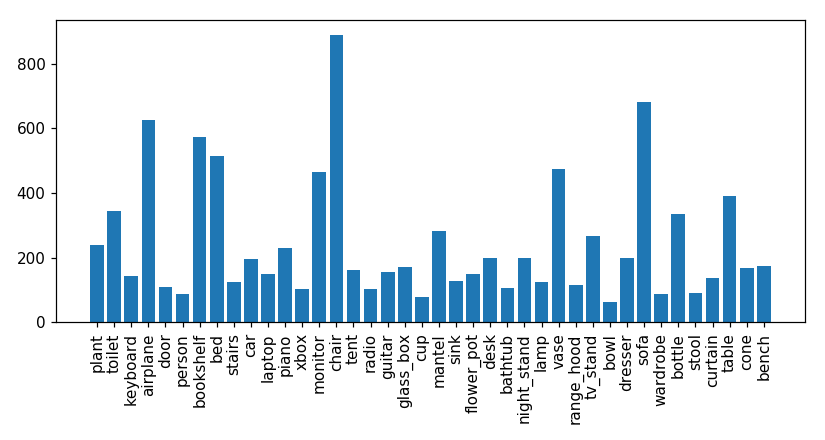
\includegraphics[width=\textwidth]{Figures/shape_retrieval/modelnet_classes.png}
    \caption{ModelNet40 data set: distribution of samples per class.}
    \label{fig:modelnet_classes}
\end{figure}

\subsection{Implementation details}
To demonstrate the impact that the triplet based training has on the performance of CNN descriptors
we use a deep network architecture shown in a Table~\ref{tab:net-architecture}. This network was implemented in PySparseConvNet, which is our modification of the SparseConvNet library \cite{graham2014spatially}. Besides new loss functions PySparseConvNet can be accessed from Python for a more interactive usage.

When forming a triplet for training we choose uniformly randomly a positive pair of objects from one class
and select a negative sample uniformly randomly from one of other classes.

For the optimization we use the SGD \cite{bottou-tricks-2012}, and the training is done
\begin{itemize}
\item in batches of size from $45$ to $90$ depending on a GPU video memory,
\item with a learning rate of $0.002$,
\item and a momentum equal to $0.99$.
\end{itemize}
Training can take up to a week on a server with advanced GPU, such as NVIDIA Titan X or GTX980ti.

\begin{figure}
\centering
\begin{tabular}{ccccc}
  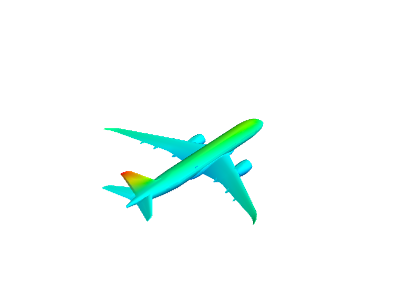
\includegraphics[width=0.19\columnwidth]{Figures/shape_retrieval/pic_airplane_solid.png} &
  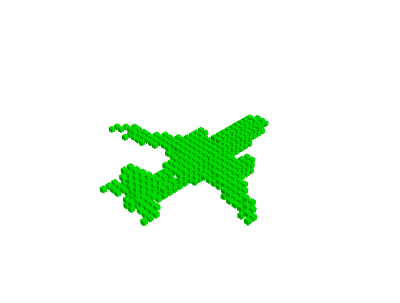
\includegraphics[width=0.19\columnwidth]{Figures/shape_retrieval/pic_airplane_30_solid.png} &
  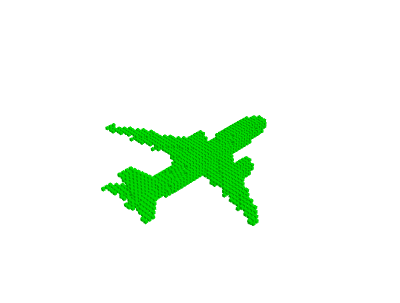
\includegraphics[width=0.19\columnwidth]{Figures/shape_retrieval/pic_airplane_50_solid.png} &
  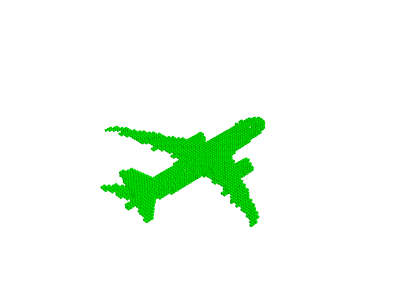
\includegraphics[width=0.19\columnwidth]{Figures/shape_retrieval/pic_airplane_70_solid.png} &
  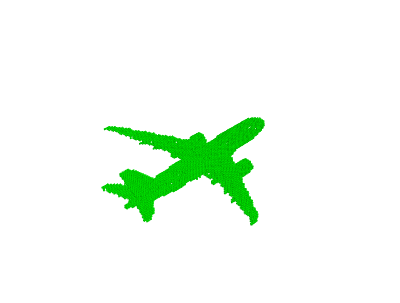
\includegraphics[width=0.19\columnwidth]{Figures/shape_retrieval/pic_airplane_100_solid.png} \\
% (a) first & (b) second \\
 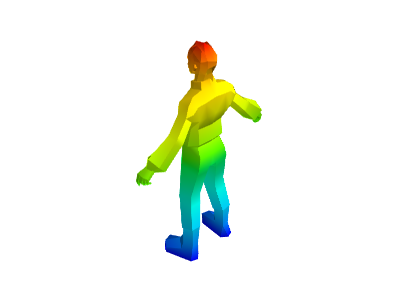
\includegraphics[width=0.19\columnwidth]{Figures/shape_retrieval/pic_person_solid.png} &
 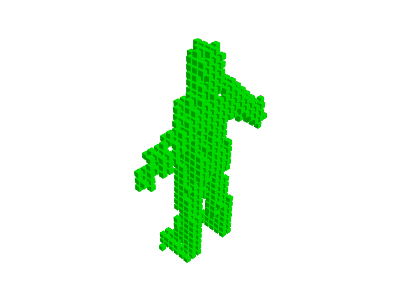
\includegraphics[width=0.19\columnwidth]{Figures/shape_retrieval/pic_person_30_solid.png} &
 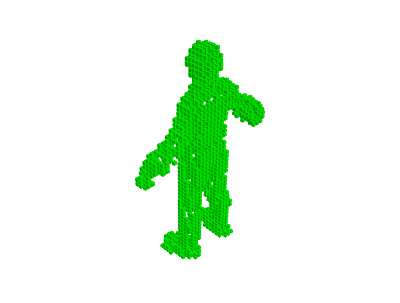
\includegraphics[width=0.19\columnwidth]{Figures/shape_retrieval/pic_person_50_solid.png} &
 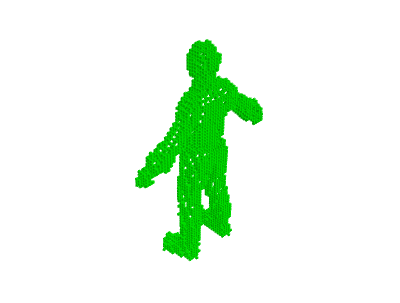
\includegraphics[width=0.19\columnwidth]{Figures/shape_retrieval/pic_person_70_solid.png} &
 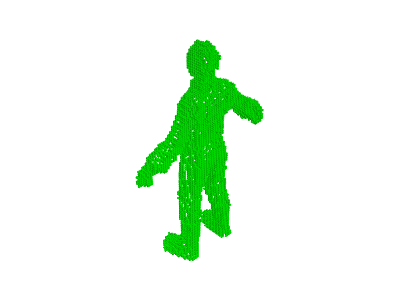
\includegraphics[width=0.19\columnwidth]{Figures/shape_retrieval/pic_person_100_solid.png} \\

 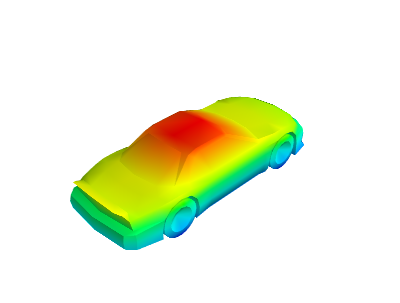
\includegraphics[width=0.19\columnwidth]{Figures/shape_retrieval/pic_car_solid.png} &
 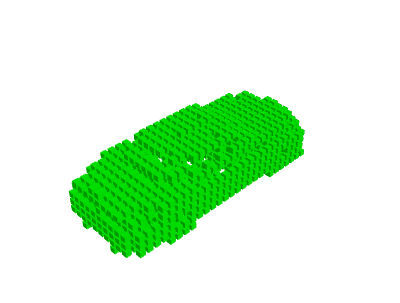
\includegraphics[width=0.19\columnwidth]{Figures/shape_retrieval/pic_car_30_solid.png} &
 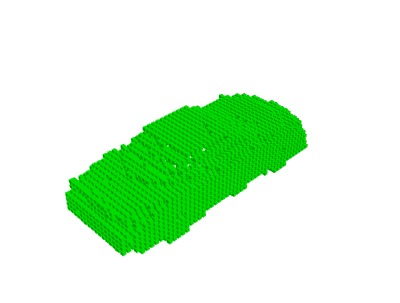
\includegraphics[width=0.19\columnwidth]{Figures/shape_retrieval/pic_car_50_solid.png} &
 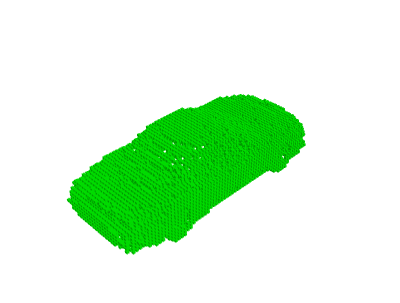
\includegraphics[width=0.19\columnwidth]{Figures/shape_retrieval/pic_car_70_solid.png} &
 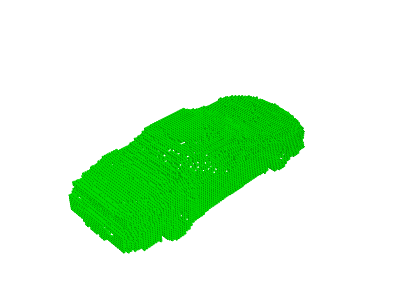
\includegraphics[width=0.19\columnwidth]{Figures/shape_retrieval/pic_car_100_solid.png} \\
\end{tabular}
\caption{Examples of some objects voxelizations at different resolutions $30$, $50$, $70$, $100$ (from left to right), left-most objects are depicted using original meshes}
\label{fig:voxels-examples}
\end{figure}


We train Sparse 3D Convolutional Neural Network (S3DCNN) on the 3D shape classification dataset by splitting it into  training and validation subsets, adding augmentation of data to achieve rotational and translational invariance. After training a model on a dataset of pairs, we use it to embed voxel representations of 3D meshes into $192$-dimensional space. The retrieval consist of ranking search objects by a cosine distance of vectors from a query vector.

The most popular metrics for evaluating retrieval performance are
\begin{itemize}
\item Precision-Recall Curve shows a trade-off between these two measures and how quickly the precision drops with the recall increase,
\item Mean average precision (mAP). Given a query, its average precision is the average of all precision values computed on all relevant objects in the retrieved list. Given several queries, the mean average precision (mAP) is the mean of average precisions for these queries. 
\end{itemize}
We evaluated mAP for different voxel rendering sizes of 3D shapes both at train and test times, see also Figure~\ref{fig:voxels-examples}.

To check if our model is comparable with other architectures, we consider a classification task. So, we trained our model for the classification task using the ModelNet40 train subset with 
\begin{itemize}
\item SoftMax last layer for $200$ epochs,
\item with exponentially discounting learning rate,
\item and performed retrieval evaluation on the test subset,
\item taking $20$ images from every class, and ranking them w.r.t their $L2$-norm by activations taken from the $17$-th layer.
\end{itemize}

Results of these experiments are provided in Table~\ref{tab:classification}. We can see that in case of classification task setup our model is comparable in terms of the classification accuracy, but mAP values are worse. But in case of metric learning performace of S3DCNN on mAP metric is much better.
Superior performance of retrieval task with MVCNN is not a surprising result, since MVCNN uses neural nets, pre-trained on ImageNet. On the other hand our model only requires 3D Shape dataset to learn.

In Figure~\ref{fig:map_for_rs} we provide the dependence of mAP on the input spatial resolution. We can see that the retrieval performance improves with increase in the input spatial resolution up to around $45-50$, after that it drops slightly and goes to plateau. It can be attributed to the insufficient amount of layers for the same scale of features, that can be separated in higher layers. Light blue color shows range of mAP on validation for top $30$ trained architectures.


\begin{figure}[!tbp]
\vspace{-20pt}
\centering
\begin{minipage}[b]{0.45\textwidth}
  \centering
  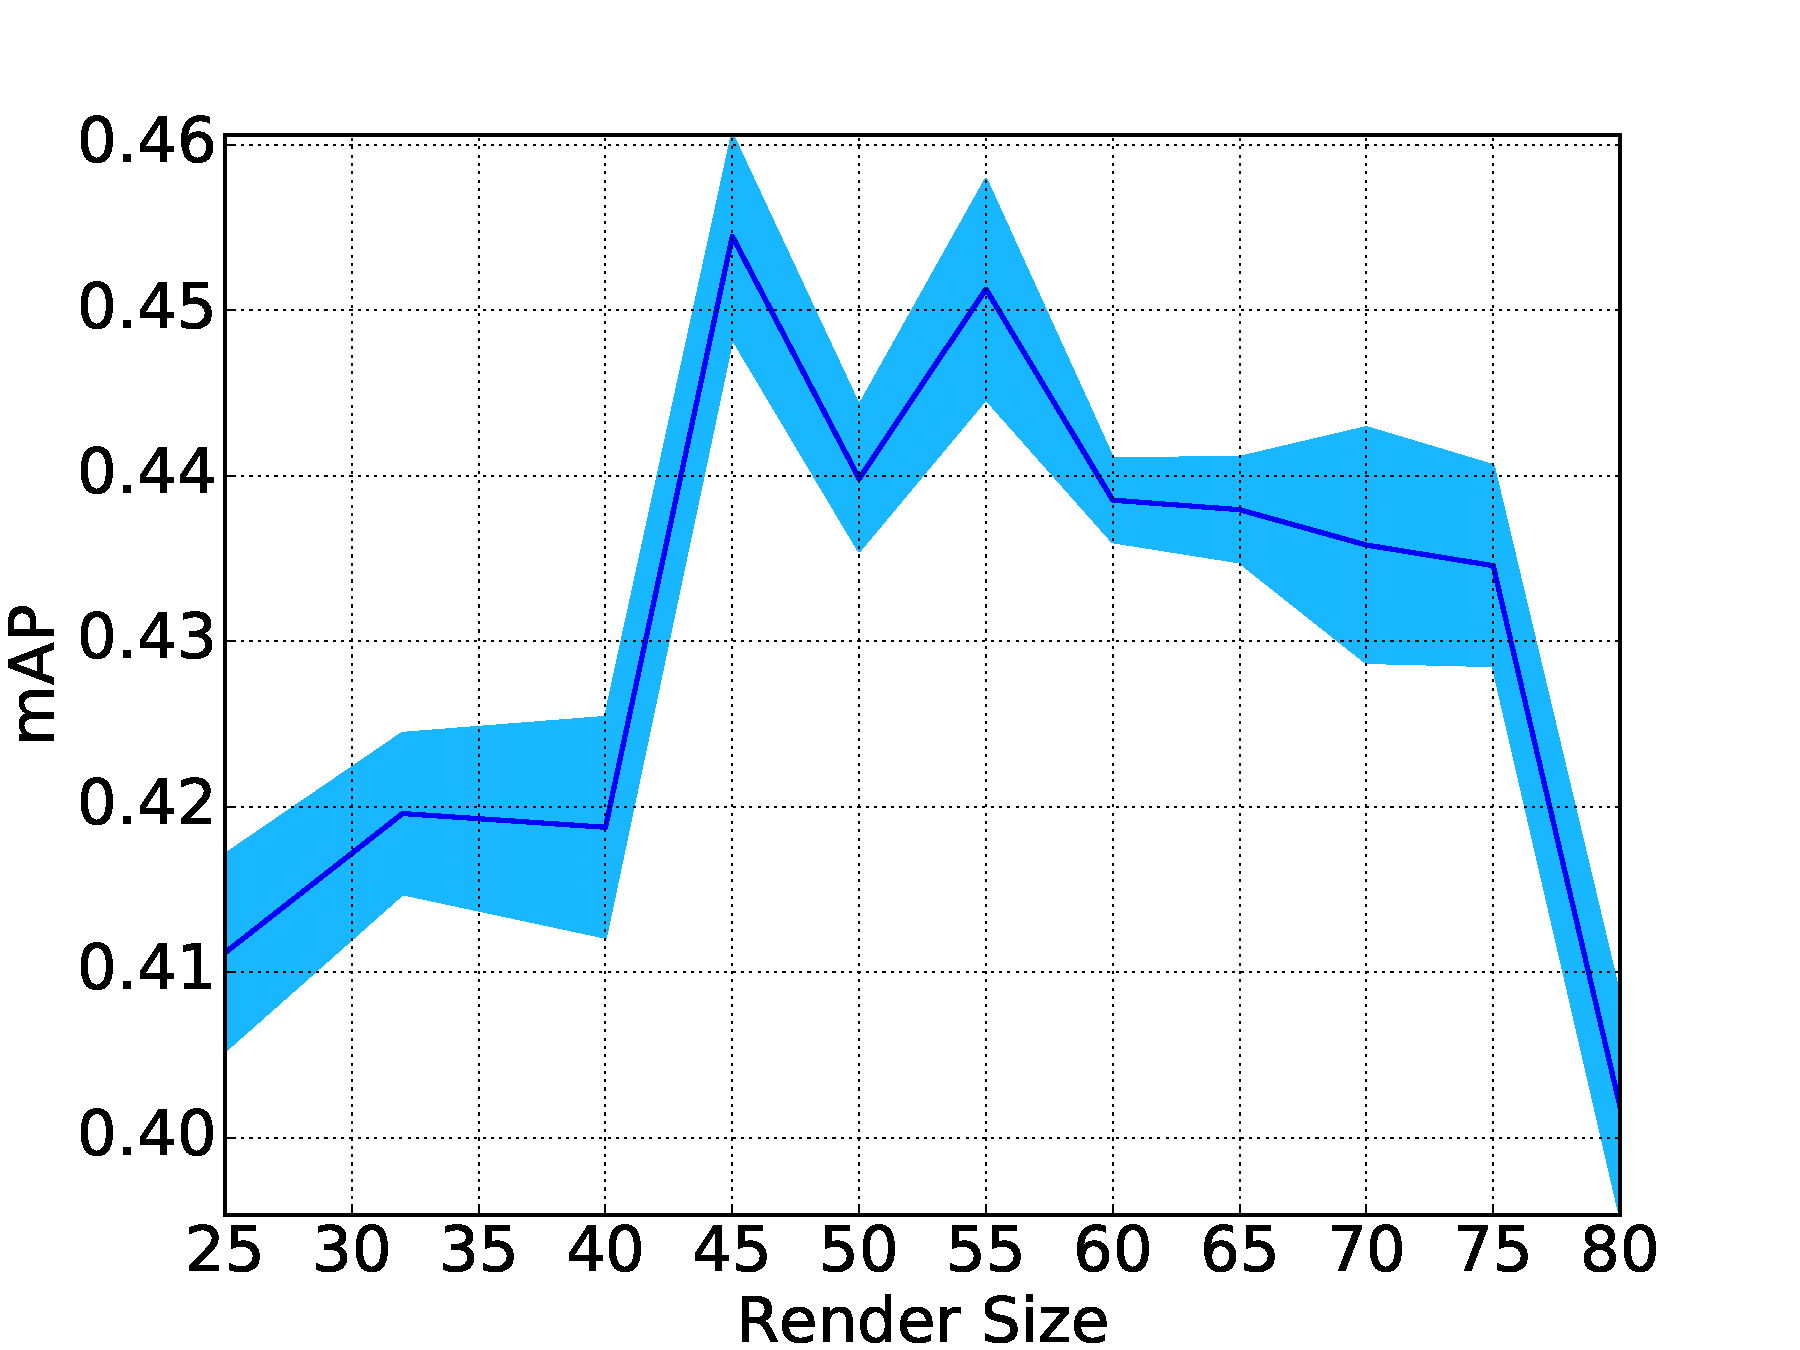
\includegraphics[width=\columnwidth]{Figures/shape_retrieval/new_map_to_rs.pdf}
  \caption{Dependence of the retrieval performance on the input spatial resolution}
  \label{fig:map_for_rs}
\end{minipage}
\begin{minipage}[b]{0.45\textwidth}
  \centering
  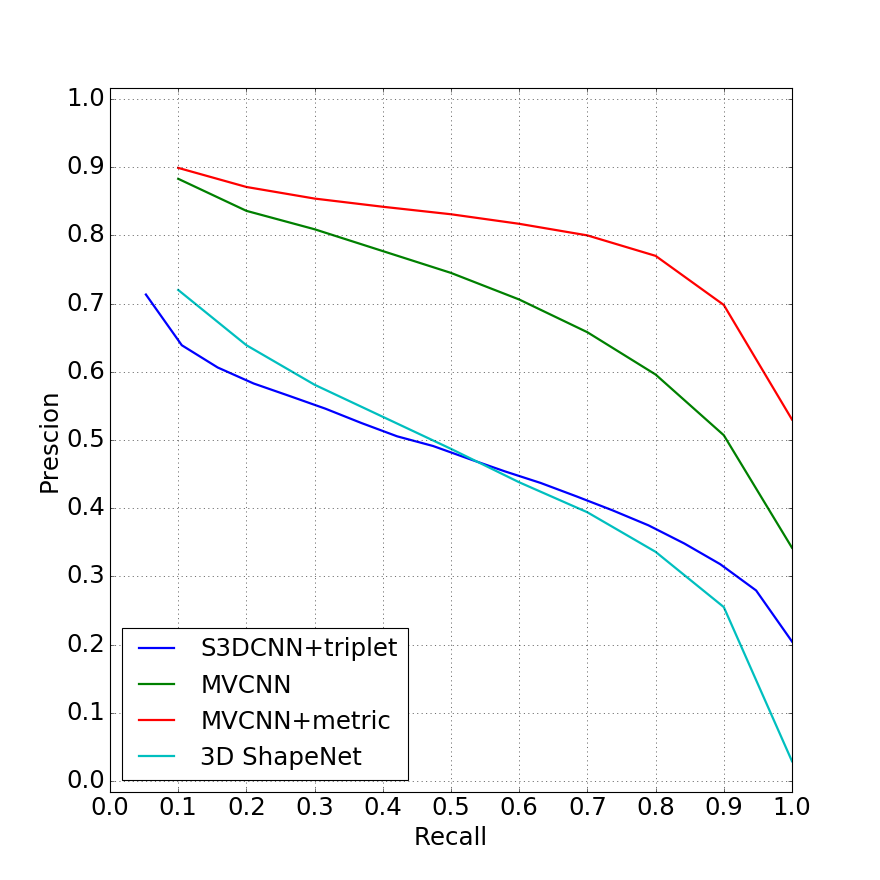
\includegraphics[width=\columnwidth]{Figures/shape_retrieval/pr_curves_comp}
  \caption{Precision-Recall curve for our method}
  \label{fig:pr_curve}
\end{minipage}
\end{figure}


We would like to note that in Figure~\ref{fig:map_for_rs} mAP values provided for different validation epochs and variability of best model can be explained by difference in total learning time.

% \begin{itemize}
% \item In Table~\ref{tab:classification} for the retrieval we used features from the last but one layer of the network,
% \item In Figure~\ref{fig:map_for_rs} we used learning with the triplet loss, for which we still have to better adjust the architecture and learning rate schedule.
% \end{itemize}


\section{Results}
\label{sec:5}

\begin{figure}
  \centering
    \includegraphics[width=\textwidth]{Figures/shape_retrieval/cnn_embed_2k.jpg}
    \caption{t-SNE plot of ModelNet40 validation set}
    \label{fig:modelnet_tsne}
\end{figure}

We found that the retrieval performance improves with increase in the input spatial resolution. However, such an effect is difficult to check experimentally and to use in practice, as e.g. for usual 3D dense CNNs the computational time is prohibitively large. In our case, data sparsity helps us to process data in reasonable time even with input resolution up to $100^3$ voxels, therefore we can benefit from the increase of the input spatial resolution when performing retrieval.
In Figure~\ref{fig:pr_curve} we can see that our method is comparable to \cite{wu20153d} in low recall, and better at higher recall values, that indicates better scalability of our method.
In Table~\ref{tab:classification} for the retrieval we used features from the one before last layer of the network of size 192, which in  comparison to 4000 in 3DShapeNet model \cite{wu20153d} is 20 times smaller but achieves almost the same retrieval metrics.


We evaluated our network architecture described in Table~\ref{tab:net-architecture} on popular state-of-the-art frameworks for Deep Learning, such as Tensorflow~\cite{tensorflow2015-whitepaper} on GPU and \cite{2016arXiv160502688short} on CPU.
Using Keras \cite{chollet2015keras} 2.0.2 with Tensorflow~\cite{tensorflow2015-whitepaper} 1.2.1 backend on Nvidia Titan X GPU with 12Gb of GPU memory, we were able to exhaust all of it with batch size equal to 12, and performed forward passes on average 0.0301 seconds/sample, which is comparable to processing speed of our implementation with render size of about 60-70.
Other setup was an implementation of our network architecture on Keras with Theano backend using Intel i7-5820K 6-core CPU processor, took 1.53 seconds/sample, which is significantly slower.
% We provide training code for all experiments in our repository\footnote{\url{https://github.com/gangiman/PySparseConvNet}}.


\begin{table}[t]
  \caption{Evaluation on Modelnet40}
  \label{tab:classification}
  \centering
  \begin{tabular}{llll}
    \toprule
    method & Classification & Retrieval AUC & Retrieval mAP \\
    \midrule
    3DShapeNet \cite{wu20153d} & 77.32\% & 49.94\% & 49.23\% \\
    MVCNN \cite{su15mvcnn} & 90.10\% & --- & 80.20\% \\
    VoxNet \cite{maturana2015voxnet} & 83.00\% & --- & --- \\
    VRN \cite{brock2016generative} & 91.33\% & --- & --- \\
    \textbf{S3DCNN (proposed)} & \textbf{90.30}\% & \textbf{36.05}\% & \textbf{33.67}\% \\
    \textbf{S3DCNN + triplet (proposed)} & --- & \textbf{48.81}\% & \textbf{46.71}\% \\
    \bottomrule
  \end{tabular}
\end{table}

\subsubsection*{Acknowledgments}
We are very grateful to Dmitry Yarotsky for his contribution to this research project. Big Thanks to Benjamin Graham for some useful comments and ideas. Thanks to Rasim Akhunzyanov for his help in debugging the PySparseConvNet code.

The research was partially supported by the Russian Science Foundation grant (project 14-50-00150).

% \clearpage
% \bibliographystyle{abbrv}
% \bibliography{bibliography}

% \end{document}

\newpage 
% \documentclass[10pt,twocolumn,letterpaper]{article}

% \usepackage[dvipsnames]{xcolor}
% \usepackage{cvpr}
% \usepackage{times}
% \usepackage{epsfig}
% \usepackage{graphicx}[draft]
% \usepackage{amsmath}
% \usepackage{amssymb}
% \usepackage{array,colortbl,multirow,multicol,booktabs,ctable}
% \usepackage{bm}
% \usepackage{subfig}
% % The LaTeX graphics/graphicx package uses the first 
% % dot to find the extension. Package grffile changes 
% % the algorithm to check for known extensions (option multidot, enabled by default):
% \usepackage{grffile} 
% \usepackage{dblfloatfix}

% % Include other packages here, before hyperref.

% % If you comment hyperref and then uncomment it, you should delete
% % egpaper.aux before re-running latex.  (Or just hit 'q' on the first latex
% % run, let it finish, and you should be clear).
% \usepackage[pagebackref=true,breaklinks=true,letterpaper=true,colorlinks,bookmarks=false]{hyperref}

% % \cvprfinalcopy % *** Uncomment this line for the final submission

% \def\cvprPaperID{4968} % *** Enter the CVPR Paper ID here
% \def\httilde{\mbox{\tt\raisebox{-.5ex}{\symbol{126}}}}

% % Pages are numbered in submission mode, and unnumbered in camera-ready
% \ifcvprfinal\pagestyle{empty}\fi

% \renewcommand{\floatpagefraction}{.9}
% \renewcommand{\textfraction}{.1}

% \renewcommand{\baselinestretch}{0.955}
% \renewcommand{\paragraph}[1]{\noindent{\bf #1}}

% \begin{document}

% %%%%%%%%% TITLE
% \title{Perceptually-Based Single-Image Depth Super-Resolution}
\chapter{Perceptually-Based Single-Image Depth Super-Resolution}

% \author{First Author\\
% Institution1\\
% Institution1 address\\
% {\tt\small firstauthor
% @i1.org}
% % For a paper whose authors are all at the same institution,
% % omit the following lines up until the closing ``}''.
% % Additional authors and addresses can be added with ``\and'',
% % just like the second author.
% % To save space, use either the email address or home page, not both
% \and
% Second Author\\
% Institution2\\
% First line of institution2 address\\
% {\tt\small secondauthor@i2.org}
% }

% \maketitle
% %\thispagestyle{empty}
\input Chapters/depth_superresolution/00-pre.tex

% %%%%%%%%% ABSTRACT
% \begin{abstract}
% RGBD images, combining high-resolution color and lower-resolution depth from various types of depth sensors, are increasingly common. One can significantly improve the resolution of depth images by taking advantage of color information; deep learning methods make combining color and depth information particularly easy. 
% However, fusing these two sources of data may lead to a variety of artifacts.  If depth maps are used to reconstruct 3D shapes, e.g., for virtual reality applications, the visual quality of upsampled images is particularly important.  To achieve high-quality results, visual metric need to be taken into account. 
% The main idea of our approach is to measure the quality of depth map upsampling using renderings of
% resulting 3D surfaces.  We demonstrate that a simple visual appearance-based loss, when used with either a trained CNN or simply a deep prior, yields significantly improved 3D shapes, as measured by a number of existing perceptual metrics. We compare this approach with a number of existing optimization and learning-based techniques.
% \end{abstract}

%%%%%%%%% BODY TEXT
\input Chapters/depth_superresolution/01-motivation.tex
% \input Chapters/depth_superresolution/02-related.tex
\input Chapters/depth_superresolution/03-visual.tex
\input Chapters/depth_superresolution/04-methods.tex
\input Chapters/depth_superresolution/05-exper.tex
\input Chapters/depth_superresolution/06-concl.tex





% Please follow the steps outlined below when submitting your manuscript to
% the IEEE Computer Society Press.  This style guide now has several
% important modifications (for example, you are no longer warned against the
% use of sticky tape to attach your artwork to the paper), so all authors
% should read this new version.

% %-------------------------------------------------------------------------
% \subsection{Language}

% All manuscripts must be in English.

% \subsection{Dual submission}

% Please refer to the author guidelines on the CVPR 2018 web page for a
% discussion of the policy on dual submissions.

% \subsection{Paper length}
% Papers, excluding the references section,
% must be no longer than eight pages in length. The references section
% will not be included in the page count, and there is no limit on the
% length of the references section. For example, a paper of eight pages
% with two pages of references would have a total length of 10 pages.
% {\bf There will be no extra page charges for CVPR 2018.}

% Overlength papers will simply not be reviewed.  This includes papers
% where the margins and formatting are deemed to have been significantly
% altered from those laid down by this style guide.  Note that this
% \LaTeX\ guide already sets figure captions and references in a smaller font.
% The reason such papers will not be reviewed is that there is no provision for
% supervised revisions of manuscripts.  The reviewing process cannot determine
% the suitability of the paper for presentation in eight pages if it is
% reviewed in eleven.  

% %-------------------------------------------------------------------------
% \subsection{The ruler}
% The \LaTeX\ style defines a printed ruler which should be present in the
% version submitted for review.  The ruler is provided in order that
% reviewers may comment on particular lines in the paper without
% circumlocution.  If you are preparing a document using a non-\LaTeX\
% document preparation system, please arrange for an equivalent ruler to
% appear on the final output pages.  The presence or absence of the ruler
% should not change the appearance of any other content on the page.  The
% camera ready copy should not contain a ruler. (\LaTeX\ users may uncomment
% the \verb'\cvprfinalcopy' command in the document preamble.)  Reviewers:
% note that the ruler measurements do not align well with lines in the paper
% --- this turns out to be very difficult to do well when the paper contains
% many figures and equations, and, when done, looks ugly.  Just use fractional
% references (e.g.\ this line is $095.5$), although in most cases one would
% expect that the approximate location will be adequate.

% \subsection{Mathematics}

% Please number all of your sections and displayed equations.  It is
% important for readers to be able to refer to any particular equation.  Just
% because you didn't refer to it in the text doesn't mean some future reader
% might not need to refer to it.  It is cumbersome to have to use
% circumlocutions like ``the equation second from the top of page 3 column
% 1''.  (Note that the ruler will not be present in the final copy, so is not
% an alternative to equation numbers).  All authors will benefit from reading
% Mermin's description of how to write mathematics:
% \url{http://www.pamitc.org/documents/mermin.pdf}.


% \subsection{Blind review}

% Many authors misunderstand the concept of anonymizing for blind
% review.  Blind review does not mean that one must remove
% citations to one's own work---in fact it is often impossible to
% review a paper unless the previous citations are known and
% available.

% Blind review means that you do not use the words ``my'' or ``our''
% when citing previous work.  That is all.  (But see below for
% techreports.)

% Saying ``this builds on the work of Lucy Smith [1]'' does not say
% that you are Lucy Smith; it says that you are building on her
% work.  If you are Smith and Jones, do not say ``as we show in
% [7]'', say ``as Smith and Jones show in [7]'' and at the end of the
% paper, include reference 7 as you would any other cited work.

% An example of a bad paper just asking to be rejected:
% \begin{quote}
% \begin{center}
%     An analysis of the frobnicatable foo filter.
% \end{center}

%   In this paper we present a performance analysis of our
%   previous paper [1], and show it to be inferior to all
%   previously known methods.  Why the previous paper was
%   accepted without this analysis is beyond me.

%   [1] Removed for blind review
% \end{quote}


% An example of an acceptable paper:

% \begin{quote}
% \begin{center}
%      An analysis of the frobnicatable foo filter.
% \end{center}

%   In this paper we present a performance analysis of the
%   paper of Smith \etal [1], and show it to be inferior to
%   all previously known methods.  Why the previous paper
%   was accepted without this analysis is beyond me.

%   [1] Smith, L and Jones, C. ``The frobnicatable foo
%   filter, a fundamental contribution to human knowledge''.
%   Nature 381(12), 1-213.
% \end{quote}

% If you are making a submission to another conference at the same time,
% which covers similar or overlapping material, you may need to refer to that
% submission in order to explain the differences, just as you would if you
% had previously published related work.  In such cases, include the
% anonymized parallel submission~\cite{Authors14} as additional material and
% cite it as
% \begin{quote}
% [1] Authors. ``The frobnicatable foo filter'', F\&G 2014 Submission ID 324,
% Supplied as additional material {\tt fg324.pdf}.
% \end{quote}

% Finally, you may feel you need to tell the reader that more details can be
% found elsewhere, and refer them to a technical report.  For conference
% submissions, the paper must stand on its own, and not {\em require} the
% reviewer to go to a techreport for further details.  Thus, you may say in
% the body of the paper ``further details may be found
% in~\cite{Authors14b}''.  Then submit the techreport as additional material.
% Again, you may not assume the reviewers will read this material.

% Sometimes your paper is about a problem which you tested using a tool which
% is widely known to be restricted to a single institution.  For example,
% let's say it's 1969, you have solved a key problem on the Apollo lander,
% and you believe that the CVPR70 audience would like to hear about your
% solution.  The work is a development of your celebrated 1968 paper entitled
% ``Zero-g frobnication: How being the only people in the world with access to
% the Apollo lander source code makes us a wow at parties'', by Zeus \etal.

% You can handle this paper like any other.  Don't write ``We show how to
% improve our previous work [Anonymous, 1968].  This time we tested the
% algorithm on a lunar lander [name of lander removed for blind review]''.
% That would be silly, and would immediately identify the authors. Instead
% write the following:
% \begin{quotation}
% \noindent
%   We describe a system for zero-g frobnication.  This
%   system is new because it handles the following cases:
%   A, B.  Previous systems [Zeus et al. 1968] didn't
%   handle case B properly.  Ours handles it by including
%   a foo term in the bar integral.

%   ...

%   The proposed system was integrated with the Apollo
%   lunar lander, and went all the way to the moon, don't
%   you know.  It displayed the following behaviours
%   which show how well we solved cases A and B: ...
% \end{quotation}
% As you can see, the above text follows standard scientific convention,
% reads better than the first version, and does not explicitly name you as
% the authors.  A reviewer might think it likely that the new paper was
% written by Zeus \etal, but cannot make any decision based on that guess.
% He or she would have to be sure that no other authors could have been
% contracted to solve problem B.
% \medskip

% \noindent
% FAQ\medskip\\
% {\bf Q:} Are acknowledgements OK?\\
% {\bf A:} No.  Leave them for the final copy.\medskip\\
% {\bf Q:} How do I cite my results reported in open challenges?
% {\bf A:} To conform with the double blind review policy, you can report results of other challenge participants together with your results in your paper. For your results, however, you should not identify yourself and should not mention your participation in the challenge. Instead present your results referring to the method proposed in your paper and draw conclusions based on the experimental comparison to other results.\medskip\\

% \begin{figure}[t]
% \begin{center}
% \fbox{\rule{0pt}{2in} \rule{0.9\linewidth}{0pt}}
%   %\includegraphics[width=0.8\linewidth]{egfigure.eps}
% \end{center}
%   \caption{Example of caption.  It is set in Roman so that mathematics
%   (always set in Roman: $B \sin A = A \sin B$) may be included without an
%   ugly clash.}
% \label{fig:long}
% \label{fig:onecol}
% \end{figure}

% \subsection{Miscellaneous}

% \noindent
% Compare the following:\\
% \begin{tabular}{ll}
%  \verb'$conf_a$' &  $conf_a$ \\
%  \verb'$\mathit{conf}_a$' & $\mathit{conf}_a$
% \end{tabular}\\
% See The \TeX book, p165.

% The space after \eg, meaning ``for example'', should not be a
% sentence-ending space. So \eg is correct, {\em e.g.} is not.  The provided
% \verb'\eg' macro takes care of this.

% When citing a multi-author paper, you may save space by using ``et alia'',
% shortened to ``\etal'' (not ``{\em et.\ al.}'' as ``{\em et}'' is a complete word.)
% However, use it only when there are three or more authors.  Thus, the
% following is correct: ``
%   Frobnication has been trendy lately.
%   It was introduced by Alpher~\cite{Alpher02}, and subsequently developed by
%   Alpher and Fotheringham-Smythe~\cite{Alpher03}, and Alpher \etal~\cite{Alpher04}.''

% This is incorrect: ``... subsequently developed by Alpher \etal~\cite{Alpher03} ...''
% because reference~\cite{Alpher03} has just two authors.  If you use the
% \verb'\etal' macro provided, then you need not worry about double periods
% when used at the end of a sentence as in Alpher \etal.

% For this citation style, keep multiple citations in numerical (not
% chronological) order, so prefer \cite{Alpher03,Alpher02,Authors14} to
% \cite{Alpher02,Alpher03,Authors14}.


% \begin{figure*}
% \begin{center}
% \fbox{\rule{0pt}{2in} \rule{.9\linewidth}{0pt}}
% \end{center}
%   \caption{Example of a short caption, which should be centered.}
% \label{fig:short}
% \end{figure*}

% %------------------------------------------------------------------------
% \section{Formatting your paper}

% All text must be in a two-column format. The total allowable width of the
% text area is $6\frac78$ inches (17.5 cm) wide by $8\frac78$ inches (22.54
% cm) high. Columns are to be $3\frac14$ inches (8.25 cm) wide, with a
% $\frac{5}{16}$ inch (0.8 cm) space between them. The main title (on the
% first page) should begin 1.0 inch (2.54 cm) from the top edge of the
% page. The second and following pages should begin 1.0 inch (2.54 cm) from
% the top edge. On all pages, the bottom margin should be 1-1/8 inches (2.86
% cm) from the bottom edge of the page for $8.5 \times 11$-inch paper; for A4
% paper, approximately 1-5/8 inches (4.13 cm) from the bottom edge of the
% page.

% %-------------------------------------------------------------------------
% \subsection{Margins and page numbering}

% All printed material, including text, illustrations, and charts, must be kept
% within a print area 6-7/8 inches (17.5 cm) wide by 8-7/8 inches (22.54 cm)
% high.



% %-------------------------------------------------------------------------
% \subsection{Type-style and fonts}

% Wherever Times is specified, Times Roman may also be used. If neither is
% available on your word processor, please use the font closest in
% appearance to Times to which you have access.

% MAIN TITLE. Center the title 1-3/8 inches (3.49 cm) from the top edge of
% the first page. The title should be in Times 14-point, boldface type.
% Capitalize the first letter of nouns, pronouns, verbs, adjectives, and
% adverbs; do not capitalize articles, coordinate conjunctions, or
% prepositions (unless the title begins with such a word). Leave two blank
% lines after the title.

% AUTHOR NAME(s) and AFFILIATION(s) are to be centered beneath the title
% and printed in Times 12-point, non-boldface type. This information is to
% be followed by two blank lines.

% The ABSTRACT and MAIN TEXT are to be in a two-column format.

% MAIN TEXT. Type main text in 10-point Times, single-spaced. Do NOT use
% double-spacing. All paragraphs should be indented 1 pica (approx. 1/6
% inch or 0.422 cm). Make sure your text is fully justified---that is,
% flush left and flush right. Please do not place any additional blank
% lines between paragraphs.

% Figure and table captions should be 9-point Roman type as in
% Figures~\ref{fig:onecol} and~\ref{fig:short}.  Short captions should be centred.

% \noindent Callouts should be 9-point Helvetica, non-boldface type.
% Initially capitalize only the first word of section titles and first-,
% second-, and third-order headings.

% FIRST-ORDER HEADINGS. (For example, {\large \bf 1. Introduction})
% should be Times 12-point boldface, initially capitalized, flush left,
% with one blank line before, and one blank line after.

% SECOND-ORDER HEADINGS. (For example, { \bf 1.1. Database elements})
% should be Times 11-point boldface, initially capitalized, flush left,
% with one blank line before, and one after. If you require a third-order
% heading (we discourage it), use 10-point Times, boldface, initially
% capitalized, flush left, preceded by one blank line, followed by a period
% and your text on the same line.

% %-------------------------------------------------------------------------
% \subsection{Footnotes}

% Please use footnotes\footnote {This is what a footnote looks like.  It
% often distracts the reader from the main flow of the argument.} sparingly.
% Indeed, try to avoid footnotes altogether and include necessary peripheral
% observations in
% the text (within parentheses, if you prefer, as in this sentence).  If you
% wish to use a footnote, place it at the bottom of the column on the page on
% which it is referenced. Use Times 8-point type, single-spaced.


% %-------------------------------------------------------------------------
% \subsection{References}

% List and number all bibliographical references in 9-point Times,
% single-spaced, at the end of your paper. When referenced in the text,
% enclose the citation number in square brackets, for
% example~\cite{Authors14}.  Where appropriate, include the name(s) of
% editors of referenced books.

% \begin{table}
% \begin{center}
% \begin{tabular}{|l|c|}
% \hline
% Method & Frobnability \\
% \hline\hline
% Theirs & Frumpy \\
% Yours & Frobbly \\
% Ours & Makes one's heart Frob\\
% \hline
% \end{tabular}
% \end{center}
% \caption{Results.   Ours is better.}
% \end{table}

% %-------------------------------------------------------------------------
% \subsection{Illustrations, graphs, and photographs}

% All graphics should be centered.  Please ensure that any point you wish to
% make is resolvable in a printed copy of the paper.  Resize fonts in figures
% to match the font in the body text, and choose line widths which render
% effectively in print.  Many readers (and reviewers), even of an electronic
% copy, will choose to print your paper in order to read it.  You cannot
% insist that they do otherwise, and therefore must not assume that they can
% zoom in to see tiny details on a graphic.

% When placing figures in \LaTeX, it's almost always best to use
% \verb+\includegraphics+, and to specify the  figure width as a multiple of
% the line width as in the example below
% {\small\begin{verbatim}
%   \usepackage[dvips]{graphicx} ...
%   \includegraphics[width=0.8\linewidth]
%                   {myfile.eps}
% \end{verbatim}
% }


% %-------------------------------------------------------------------------
% \subsection{Color}

% Please refer to the author guidelines on the CVPR 2018 web page for a discussion
% of the use of color in your document.

% %------------------------------------------------------------------------
% \section{Final copy}

% You must include your signed IEEE copyright release form when you submit
% your finished paper. We MUST have this form before your paper can be
% published in the proceedings.

% Please direct any questions to the production editor in charge of these
% proceedings at the IEEE Computer Society Press: Phone (714) 821-8380, or
% Fax (714) 761-1784.


% \clearpage
% \newpage

% {\small
% \bibliographystyle{ieee}
% \bibliography{egbib}
% }

% \clearpage
% \newpage
% \input 07-supp.tex

% \end{document}

\newpage 
% \documentclass[10pt,twocolumn,letterpaper]{article}

% \usepackage{wacv}
% \usepackage{times}
% \usepackage{epsfig}
% \usepackage{graphicx}
% \usepackage{amsmath}
% \usepackage{amssymb}
% \usepackage{placeins}
% % \usepackage{authblk}

% % Include other packages here, before hyperref.



% %%%%%%%%%%%%%%%%%%%%%%%%%%%%%%%%%%%%%%%%%%%%%%%%%%%%%%%%%%%%%%%%%%%%%%%%%%%%%%%%
% %
% %%% IMPORTANT - These next three lines are crucial.
% %               (1) PLEASE enter your paper ID (given by CMT) replacing the
% %                   '****' right below here with the ID from CMT.
% %               (2) Leave the \wacvfinacopy commented out for the submission
% %                   version, but UNCOMMENT it for your CAMERA-READY upload.
% %               (3) For the camera-ready version, you may be asked to set a
% %                   starting page number.  If so, replace the '9876' below with
% %                   the starting page number assigned by the publication chair.
 
% %(1)
% \def\wacvPaperID{410} % Enter the WACV Paper ID here

% %(2)
% \wacvfinalcopy % *** Uncomment this line for the final submission

% %(3)
% \ifwacvfinal
% \def\assignedStartPage{1} % *** Enter the assigned starting page number (instead of 9876)
% \fi

% %%%%%%%%%%%%%%%%%%%%%%%%%%%%%%%%%%%%%%%%%%%%%%%%%%%%%%%%%%%%%%%%%%%%%%%%%%%%%%%%

% % If you comment hyperref and then uncomment it, you should delete
% % egpaper.aux before re-running latex.  (Or just hit 'q' on the first latex
% % run, let it finish, and you should be clear).
% % \usepackage{hyperref}
% \ifwacvfinal
% \usepackage{hyperref}
% \hypersetup{breaklinks=true,bookmarks=false}
% \else
% \usepackage{hyperref}
% \hypersetup{pagebackref=true,breaklinks=true,colorlinks,bookmarks=false}
% \fi

% % Pages are numbered in submission mode, and unnumbered in camera-ready
% \ifwacvfinal
% \setcounter{page}{\assignedStartPage}
% \else
% \pagestyle{empty}
% \fi

% \def\httilde{\mbox{\tt\raisebox{-.5ex}{\symbol{126}}}}

% \begin{document}

%%%%%%%%% TITLE
% \title{Making DensePose fast and light}
\chapter{Making DensePose fast and light}

% \author{
%     Ruslan Rakhimov\textsuperscript{1}\thanks{Equal contribution}\space, 
%     Emil Bogomolov\textsuperscript{1}$^*$, 
%     Alexandr Notchenko\textsuperscript{1},\\
%     Fung Mao\textsuperscript{2}, 
%     Alexey Artemov\textsuperscript{1}, 
%     Denis Zorin\textsuperscript{1,3}, 
%     Evgeny Burnaev\textsuperscript{1}\\
%     \textsuperscript{1}{\small Skolkovo Institute of Science and Technology}\\
%     \textsuperscript{2}{\small Huawei Moscow Research Center (Russia)}\\
%     \textsuperscript{3}{\small New York University}\\
%     {\tt\small\{ruslan.rakhimov, e.bogomolov, alexandr.notchenko\}@skoltech.ru,}\\
%     {\tt\small fung.mao@huawei.com, a.artemov@skoltech.ru, dzorin@cs.nyu.edu, e.burnaev@skoltech.ru}\\
% }

% \author{%
%     Ruslan Rakhimov\textsuperscript{1}\thanks{Equal contribution} \\
%     {\tt\small ruslan.rakhimov@skoltech.ru}
%     \and
%     Emil Bogomolov\textsuperscript{1}$^*$ \\
%     {\tt\small e.bogomolov@skoltech.ru}
%     \and
%     Alexandr Notchenko\textsuperscript{1} \\
%     {\tt\small alexandr.notchenko@skolkovotech.ru}
%     \and
%     Fung Mao\textsuperscript{2} \\
%     {\tt\small fung.mao@huawei.com}
%     \and
%     Alexey Artemov\textsuperscript{1} \\
%     {\tt\small a.artemov@skoltech.ru}
%     \and\and\and
%     Denis Zorin\textsuperscript{1,3} \\
%     {\tt\small dzorin@cs.nyu.edu}
%     \and\and\and
%     Evgeny Burnaev\textsuperscript{1} \\
%     {\tt\small e.burnaev@skoltech.ru}
%     \and\and\and
%     \textsuperscript{1}{\small Skolkovo Institute of Science and Technology}\\
%     \textsuperscript{2}{\small Huawei Moscow Research Center (Russia)}\\
%     \textsuperscript{3}{\small New York University}
% }

% \author[1]{Ruslan Rakhimov\thanks{Equal contribution}}
% \author[1]{Emil Bogomolov$^*$}
% \author[1]{Alexandr Notchenko}
% \author[2]{Fung Mao}
% \author[1]{Alexey Artemov}
% \author[1,3]{Denis Zorin}
% \author[1]{Evgeny Burnaev}

% \affil[1]{Skolkovo Institute of Science and Technology,\{ruslan.rakhimov,e.bogomolov,alexandr.notchenko,a.artemov,e.burnaev\}}
% \affil[2]{Huawei Moscow Research Center (Russia)}
% \affil[3]{New York University}


% \affil[1]{University of Southern California, Los Angeles, CA \authorcr Email: {\tt \{uid1, uid2\}@usc.edu}\vspace{1.5ex}}
% \affil[2]{NASA Jet Propulsion Laboratory, Pasadena, CA \authorcr Email: {\tt uid3@jpl.nasa.gov} \vspace{-2ex}} 

% \author[1]{Ruslan Rakhimov\thanks{Equal contribution}\\ ruslan.rakhimov@skoltech.ru}
% \author[2]{Emil Bogomolov$^*$\\{\tt\small e.bogomolov@skoltech.ru}}
% \affil[1]{Department of Mathematics, University X}
% \affil[2]{Department of Biology, University Y}

% \maketitle
%\thispagestyle{empty}

%%%%%%%%% ABSTRACT

% \begin{abstract}
DensePose estimation task is a significant step forward for enhancing user experience computer vision applications ranging from augmented reality to cloth fitting. Existing neural network models capable of solving this task are heavily parameterized and a long way from being transferred to an embedded or mobile device. To enable Dense Pose inference on the end device with current models, one needs to support an expensive server-side infrastructure and have a stable internet connection. To make things worse, mobile and embedded devices do not always have a powerful GPU inside.
In this work, we target the problem of redesigning the DensePose R-CNN model's architecture so that the final network retains most of its accuracy but becomes more light-weight and fast. To achieve that, we tested and incorporated many deep learning innovations from recent years, specifically performing an ablation study on 23 efficient backbone architectures, multiple two-stage detection pipeline modifications, and custom model quantization methods. 
As a result, we achieved $17\times$ model size reduction and $2\times$ latency improvement compared to the baseline model.\ifwacvfinal\footnote{Code is available at \url{https://github.com/zetyquickly/DensePoseFnL}}\fi
\end{abstract}
% \section{Introduction}

This work is dedicated to developing an architecture for solving DensePose \cite{densepose} estimation task with a particular requirement: the model should be light-weight and run in real-time on a mobile device.

The task of understanding humans in an image may involve different formulations of the problem: 2d landmarks localization, human part segmentation, 3d reconstruction, dense image-to-surface correspondences (DensePose). In this work, we target the multi-person formulation of DensePose task: given a single RGB image solve the regression task: for each pixel, find its surface points (UV coordinates) on a deformable surface model (the Skinned Multi-Person Linear (SMPL) model \cite{smpl}).

Finding surface correspondence is a step forward to a general 3d human representation. Possible applications lie in such fields, like augmented reality, virtual fitting rooms. Densepose output may serve as input to another model. For instance, it was used as an input in video-to-video translation tasks \cite{vid2vid}.

Besides the original pioneering work \cite{densepose}, which introduces a carefully annotated COCO-DensePose dataset with sparse image-to-surface ground-truth correspondences and DensePose R-CNN baseline model, other works target different formulations. Parsing R-CNN \cite{parsing}, the winner solution of the COCO 2018 Challenge DensePose Estimation task, achieves state-of-the-art performance by scrutinizing different blocks in the original DensePose R-CNN architecture. Slim DensePose \cite{denseposeslim} explores the weakly-supervised and self-supervised learning problem setting, by leveraging motion cues from videos. \cite{uncertainty} improves the performance of the model by incorporating the uncertainty estimation into the model. \cite{monkeys} shows the ability to transfer the dense pose recognition from humans to proximal animal classes such as chimpanzees without a time-consuming collection of a new dataset with new classes.

However, none of the works target the task of making the network fast and light-weight, and current solutions such as baseline DensePose R-CNN and state-of-the-art Parsing R-CNN introduce heavily parametrized models.

Make the network perform near to a real-time mode is a particularly important step if we want to apply these models in the mobile or embedded devices. In this work, we explore the subtle trade-off between the performance of the model and its latency.

The contributions are the following:
\begin{itemize}
    \item we created a pipeline to test neural network architectures viability for mobile deployment,
    \item we developed an architecture based on existing techniques, achieving a finally good balance between real-time speed and average precision of our model,
    \item we performed an ablation study on many different efficient backbones, particularly applied for DensePose task.
\end{itemize} 
% \section{Related work}

\noindent 
\textbf{DensePose task.} DensePose-COCO dataset contains a large set of images of people collected ``in the wild'' together with different annotations: (i) bounding boxes, (ii) foreground-background masks, (iii) dense correspondences --- points $p \in S$ of a reference 3D model $S\in\mathbb{R}^3$ of the object associated with triplets $(c, u, v) \in\{1, \ldots, C\} \times[0,1]^{2}$, where $c$ indicates which one of $C$ body parts contains the pixel and $(u,v)$ represents the corresponding location (UV coordinates) in the chart of the part \cite{smpl}.
The DensePose task is then to predict such triplets $(c, u, v)$ for each foreground pixel and every person in the image.
\newline

\noindent \textbf{DensePose R-CNN.} The baseline dense pose prediction model, and all the subsequent works \cite{parsing, uncertainty, monkeys} follow the architecture design of Mask R-CNN \cite{maskrcnn}.

The model is a two-stage: first, it generates class-independent region proposals (boxes), then classifies and refines them using the box/class head. Finally, the DensePose head predicts the body part and UV coordinates for each pixel inside the box. Particularly, the model consists of many different blocks (see Fig.~\ref{fig:scheme}):
\begin{itemize}
    \item \textit{Backbone} to extract features from the image,
    \item \textit{Neck} to integrate features from different feature levels of the backbone to effectively perform multi-scale detection,
    \item \textit{Region proposal network (RPN)} to propose a sparse set of box candidates potentially containing objects,
    \item \textit{Heads} take the features pooled from the bounding box on the corresponding feature level, where the detection occurred, and produce output. The first head is a box/class head, which finally predicts whether the object is present in the box and refines the box coordinates. The second head is the DensePose head that predicts either the pixel belongs to the background or assigns it to one of the 24 DensePose charts, and regresses UV coordinates to each foreground pixel inside the bounding box.
\end{itemize}

\noindent \textbf{Model architecture optimisation.}
In recent years the neural architecture search (NAS) techniques gained popularity \cite{automl}. The main aim of NAS is to find the optimal architecture under specific hardware requirements. Usually, these techniques are applied in simple setups, e.g., classification networks, or in the case of two-stage object detection models, NAS is usually applied to individual parts of the model \cite{nasfpn}. In this paper, instead of creating one more design for a particular part of the model, we try to test different existing approaches and see what works best for the DensePose estimation task. Particularly, we evaluate several backbones that were a result of NAS optimization and try to test them out with other components.

\begin{figure}[!hbtp]
\centering
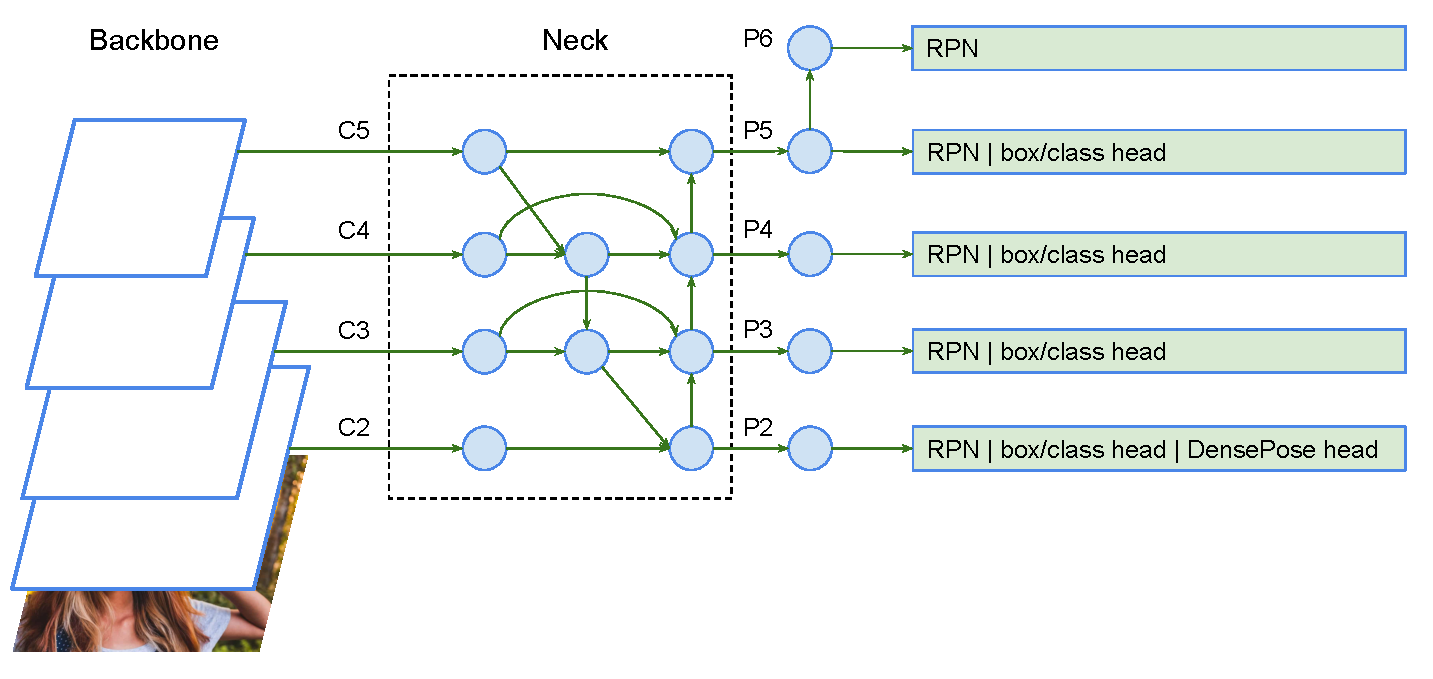
\includegraphics[width=0.4\textwidth]{images/scheme.pdf}
\caption{The high level structure of the Mobile Parsing R-CNN model. $C_i$, $P_i$ represent feature levels with a resolution of $1/2^i$ of the input image. $P_6$ is obtained via stride-2 pooling on $P_5$.}
\label{fig:scheme}
\end{figure}
\section{Mobile Parsing R-CNN}
\label{section3}

In this section, we address the design choice of different parts inside our model, which we call Mobile Parsing R-CNN. In general, the model's design follows the Parsing R-CNN model, the winner solution of the COCO 2018 Challenge DensePose Estimation task, but with different modifications in different parts.

\subsection{Backbone}

While there are many different possible designs of a backbone network, we target efficient models with a block structure as that in MobileNetV1 and V2 \cite{mobilenetv1, mobilenetv2} (depth-wise separable convolutions and inverted residuals with linear bottlenecks). This base block is the foundation for most efficient backbones used today, which were selected for evaluation as the backbone of the improved model. 
Let us list various architectures we use in our experiments:
\begin{itemize}
    \item \textbf{MobileNetV3}.  \cite{mobilenetv3} applies neural architecture search (NAS) and improves MobileNetV2 by adopting Squeeze and excitation block for channel-wise attention and non-linearities like h-sigmoid and h-swish;
    \item \textbf{MixNet}. \cite{mixnet} develops a multi-kernel variant of MobileNetV2, i.e., depth-wise convolutions consisting of convolutions with different kernel sizes;
    \item \textbf{Differentiable NAS} considers the problem of finding neural architecture in a differentiable way by carefully designing search space. We consider the following models, obtained using the differentiable NAS procedure: MnasNet \cite{mnasnet}, FBNet \cite{fbnet}, Single-Path\cite{spnasnet};
    \item \textbf{EfficientNets} from \cite{efficientnetb} appear to be one of the first architectures, obtained using AutoML approaches for image classification, and achieve a good compromise between the accuracy on a classification task and the number of the parameters of the network. \cite{efficientnetb} shows that one can apply a power-law scaling of width as a function of depth. Later EfficientNets were customized for Google's Edge TPUs \cite{efficientnete} using MNAS framework \cite{mnasnet};
    \item \textbf{CondConv}. Traditional convolutional layers have the kernel weights fixed once they are trained. CondConv \cite{condconv} applies a linear combination of several kernels (a mixture of experts) with weights generated dynamically by another network based on the input. While the original work is devoted to the classification task, we explore this \textit{``dynamic''} approach combined with EfficientNets on the DensePose task.
\end{itemize}

\subsection{Neck}

The main challenge in the object detection pipeline is to be able to detect objects of different scales. Earlier detectors predict objects based on features extracted from different levels of the backbone. Later, feature pyramid network (FPN \cite{fpn}) proposes to integrate features in a top-down manner to enrich fine-grained features from the lowest level of feature pyramid with semantically rich information from deeper layers. While the original work \cite{fpn} considers only the top-down pathway for information aggregation, later works also add cross-scale connections between the feature levels. In this work, we make use of bidirectional FPN (BiFPN \cite{bifpn}) for multi-scale feature fusion, which outperforms its recent counterparts in object detection tasks (see \cite{bifpn}), while remaining light-weight and fast. It is partly achieved by using separable convolutions inside.

\subsection{Densepose head}

We increase the region of interest (RoI) resolution for the DensePose head from $14\times14$ to $32\times32$, as it was suggested in \cite{parsing}.

While the original network uses 8 convolutions layers in the DensePose head, we, instead, similar to \cite{parsing}, use the atrous spatial pyramid pooling (ASPP) \cite{aspp} module, followed by 4 convolutional layers. Also, we omit the non-local convolutional layer \cite{nonlocal} between ASPP and convolutional layers in order not to increase the latency of the network because it performs pixel to pixel comparisons resulting in $O(n^2)$ operations, where $n$ is the number of pixels.

Finally, the DensePose predictions happen on the finest level from the feature pyramid as in \cite{parsing}, while box/class predictions happen on all levels.

\subsection{Quantization of backbone layers}
\label{quant}

We proposed the quantization procedure for Parsing R-CNN based on quantization aware training tools provided by PyTorch. 
First of all, it is necessary to patch the existing network architecture. Considering the whole network operates with quantized tensors, we should find intermediate parts where floating-point tensors are crucial to obtain satisfactory results.
\begin{enumerate}
    \item RPN classification and regression heads use a $3\times3$ convolutional layer to produce a shared hidden state from which one $1\times1$ convolutional layer predicts objectness logits for each anchor, and another one predicts bounding-box deltas specifying how to refine the anchor coordinates to get a final object proposal. These layers work with quantized feature tensors, but for correct calculation of RPN proposals, predicted objectness logits and anchor deltas are dequantized after inference of bounding box predictor.
    \item To perform accurate RoI pooling, it is necessary first to dequantize input features, apply pooling, and then quantize features back.
    % \item To perform accurate box pooling, it is necessary to dequantize input features. In that case, RoI pooling would work with floating-point features and RPN proposals. After this operation, we quantize cropped feature tensors before passing them to the following layers.
\end{enumerate}

The second step is fusion. We fuse each convolutional and linear layer, followed by batch normalization and activation to one atomic layer. That is needed to save on memory access while also improving the operations' numerical accuracy.
The third step is to run the quantization aware training of the patched and fused model.
% The last step is to perform an evaluation of the resulted model.

During the second and third steps, we run into design obstacles that are described below.

In BiFPN architecture, we collect features before point-wise linear convolutions using pre-forward hooks. This allows us to link to this layer's input rather than to the output of the input provider. But quantization tools implemented in the PyTorch framework at this stage do not allow this to be done. We proposed a mechanism that preserves pre- and post- forward hooks during fusion and preparation for quantization and does not harm the quality of the quantization process itself. The diagram of the proposed mechanism is in Fig.~\ref{fig:preserve_hooks}.

\begin{figure}[!hbtp]
\centering
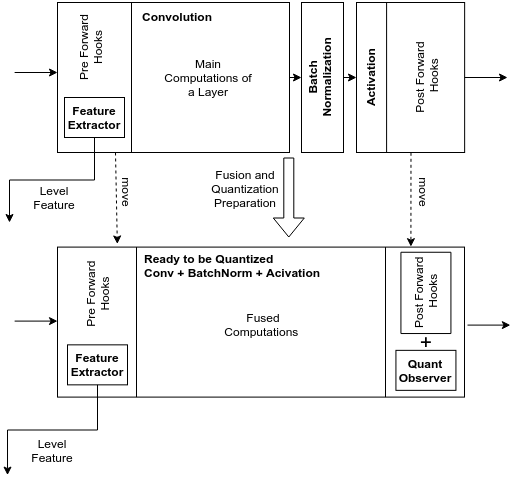
\includegraphics[width=0.4\textwidth]{Figures/densepose/diagram.png}
\caption{The feature collection scheme for quantized models.}
\label{fig:preserve_hooks}
\end{figure}
\section{Experiments}

In this section, we provide the experimental results on design choices for different parts of the model. The majority of experiments are done on the cluster, and finally, we transfer the model to a mobile device to check the performance there.

\subsection{Implementation details}

The models were implemented in PyTorch using Detectron2 \cite{detectron2} platform.

We choose hyper-parameters matching to those in Parsing R-CNN\cite{parsing}, i.e., we use a batch of 16 images (2 images per GPU), therefore we apply synchronous batch normalization \cite{syncbn} instead of usual batch normalization wherever it is used inside the backbone and neck. We use no normalization in box/class and dense pose heads. We sample 512 RoIs for box/class head and 32 RoIs for dense pose head. By default, we train models for 130k iterations with initial learning rate 0.002, decreasing it by 10 at 100k and 120k iterations. Under such a schedule, training of one model takes approximately 1 day on 8 NVIDIA Tesla V100 GPUs. Since all models are quite small, the memory consumption during training allows to decrease the number of GPUs for parallel training. Unless specified otherwise, by default, we scale images in a way that shortest image size equals 800 pixels during the inference stage. Each model's backbone is initialized with weights of the corresponding network trained on the ImageNet classification task. We train models on a combination of \textit{train} and \textit{valminusminival} partitions of Densepose-COCO dataset \cite{densepose} and test them on a \textit{minival} partition.


\subsection{Metrics}
Following the original work, we use as evaluation metric the Average Precision (AP) at a number of \textit{geodesic point similarity} (GPS) thresholds ranging from 0.5 to 0.95. We also report box average precision.

As we are interested in deploying a DensePose model on a mobile device, we report the number of parameters of each model and FPS measured on CPU and GPU. In particular, we measure the inference performance of all models on the same NVIDIA GeForce GTX 1080 Ti. It is worth mentioning that the DensePose model is a two-stage model, so the FPS of the model is directly conditioned on the performance of the first stage of the model. There is a subtle trade-off between the quality and latency; as for example, the network that does not predict any instances will never run dense pose head, and vice versa, the network that produces many false-positive results would redundantly run the model heads. As the latency of the network is data-dependent, we average latency time across DensePose-COCO minival dataset and finally convert it to FPS.

\subsection{Ablation on components}

\begin{table*}[t!]
\centering
\resizebox{\textwidth}{!}{
\begin{tabular}{cllll}
 &  DensePose R-CNN (baseline) \cite{densepose} & Parsing R-CNN \cite{parsing} & Mobile Parsing R-CNN (A) & Mobile Parsing R-CNN (B) \\\hline
Backbone & ResNet-50 \cite{resnet} & ResNet-50 \cite{resnet} & Single-Path \cite{spnasnet} & Single-Path \cite{spnasnet} \\
Neck & FPN\cite{fpn} & FPN\cite{fpn} & FPN\cite{fpn} & BiFPN  \\
RoI resolution & $14\times14$ & $32\times32$ & $32\times32$ & $32\times32$ \\
Pooling Type & RoIPool & RoIPool & RoIAlign & RoIAlign \\
Box/class head & 2 linear layers & 2 linear layers & 2 conv layers & 2 conv layers \\
% test time shortest image size & 800px & 800px & 800px & 800 px\\
Feature level for prediction & $P_2$,$P_3$,$P_4$,$P_5$ & $P_2$ & $P_2$ & $P_2$ \\
DensePose head & 8 conv layers & ASPP\cite{aspp}+NL\cite{nonlocal}+4 conv layers & ASPP\cite{aspp}+4 conv layers & ASPP\cite{aspp}+4 conv layers \\
\#Channels & 512 & 512 & 256 & 64 \\
\hline
\#Params & 59.73M & 54.36M & 11.35M & 3.35M \\
GPU FPS & $13.16$ & $10.15$ & $12.03$ & $22.77$ (3x LR: $\mathbf{23.55}$) \\
CPU FPS & $1.62$ & $1.39$ & $1.42$ & $2.02$  (3x LR: $\mathbf{2.10}$) \\
box AP & $57.8$ & $59.609$ & $56.370$ & $55.39$ (3x LR: $56.83$)\\
densepose AP & $49.8$ & $54.676$ & $49.512$ & $46.79$ (3x LR: $51.08$)\\
\hline
\end{tabular}}
\caption{The main differences between the models presented. Results on DensePose-COCO minival. 3x LR refers to 3 times longer training compared to the default setting. $P_i$ represents a feature level with a resolution of $1/2^i$ of the input images. \#Channels represent the number channels inside \textit{neck} and \textit{heads}.}
\label{table:configs}
\end{table*}

% TODO describe testing pipeline

% In this section we show how we accelerated Parsing R-CNN architecture for dense pose estimation task.

% TODO highlight the differences 
\begin{table*}[t!]
\centering
\resizebox{\textwidth}{!}{
\begin{tabular}{lcccccc}
\hline
Backbone & Top-1 Accuracy (\%) & \#Params & box AP & dp. AP & GPU FPS & CPU FPS \\ \hline
ResNet-50 \cite{resnet} & $77.15$ & $33.61$M & $60.0$ & $\mathbf{54.7}$ & $11.05$ & $1.34$ \\
EfficientNet-B3 \cite{efficientnetb} & $81.636$ & $16.03$M & $59.027$ & $53.084$ & $8.31$ & $1.37$ \\
EfficientNet-EdgeTPU-L \cite{efficientnete} & $80.534$ & $17.89$M & $60.069$ & $53.378$ & $8.11$  & $1.34$ \\
MixNet-XL \cite{mixnet} & $80.120$ & $19.10$M & $58.444$ & $51.475$ & $8.54$  & $1.32$ \\
EfficientNet-B2 \cite{efficientnetb} & $79.688$ & $13.68$M & $58.041$ & $51.800$ & $9.33$ & $1.38$ \\
MixNet-L \cite{mixnet} & $78.976$ & $14.62$M & $57.481$ & $50.649$ & $8.52$ & $1.34$ \\
EfficientNet-EdgeTPU-M \cite{efficientnete} & $78.742$ & $14.57$M & $58.825$ & $52.302$ & $9.21$ & $1.37$ \\
EfficientNet-B1 \cite{efficientnetb} & $78.692$ & $13.03$M & $57.654$ & $51.053$ & $9.49$ & $1.39$ \\
CondConv-EfficientNet-B0 \cite{efficientnete, condconv} & $77.304$ & $18.32$M & $56.779$ & $49.231$ & $10.63$ & $1.40$ \\
EfficientNet-EdgeTPU-S \cite{efficientnete} & $77.264$ & $13.12$M & $58.296$ & $51.606$ & $10.03$ & $1.39$ \\
MixNet-M \cite{mixnet} & $77.256$ & $12.39$M & $56.834$ & $48.371$ & $9.39$ & $1.35$ \\
EfficientNet-B0 \cite{efficientnetb} & $76.912$ & $12.10$M & $56.271$ & $49.647$ & $10.53$ & $1.39$ \\
MixNet-S \cite{mixnet} & $75.988$ & $11.52$M & $55.132$ & $46.685$ & $10.34$ & $1.37$ \\
MobileNetV3-Large-1.0 \cite{mobilenetv3} & $75.516$ & $12.04$M & $54.537$ & $47.195$ & $11.54$ & $1.40$ \\
MnasNet-A1 \cite{mixnet} & $75.448$ & $10.94$M & $54.648$ & $47.036$ & $11.21$ & $1.38$ \\
FBNet-C \cite{fbnet} & $75.124$ & $11.49$M & $55.399$ & $47.983$ & $10.97$ & $1.37$ \\
MnasNet-B1 \cite{mnasnet} & $74.658$ & $11.31$M & $52.280$ & $47.658$ & $11.24$ & $1.37$ \\
Single-Path \cite{spnasnet} & $74.084$ & $11.35$M & $56.370$ & $49.512$ & $\mathbf{12.03}$ & $\mathbf{1.42}$ \\
MobileNetV3-Large-0.75 \cite{mobilenetv3} & $73.442$ & $10.92$M & $52.763$ & $44.736$ & $11.02$ & $1.36$ \\
MobileNetV3-Large-1.0 (minimal) \cite{mobilenetv3} & $72.244$ & $10.48$M & $52.464$ & $44.632$ & $11.33$ & $1.36$ \\
MobileNetV3-Small-1.0 \cite{mobilenetv3} & $67.918$ & $10.07$M & $49.614$ & $35.808$ & $10.62$ & $1.35$ \\
MobileNetV3-Small-0.75 \cite{mobilenetv3} & $65.718$ & $9.74$M & $44.224$ & $32.650$ & $10.16$ & $1.33$ \\
MobileNetV3-Small-1.0 (minimal) \cite{mobilenetv3} & $62.898$ & $9.58$M & $45.989$ & $36.522$ & $10.34$ & $1.34$ \\\hline
\end{tabular}}
\caption{Ablation on the backbone network used in Mobile Parsing R-CNN (A). The backbones are sorted by top-1 accuracy. Results on DensePose-COCO \textit{minival}}
\label{table:backbones}
\end{table*}

First, we implemented the Parsing R-CNN \cite{parsing} in Detectron2 following the original implementation. Then we modify the architecture exploiting the techniques presented in the Section~\ref{section3} and present two versions of a new model: Mobile Parsing R-CNN (A) and Mobile Parsing R-CNN (B). See the main architecture differences and obtained results in Table~\ref{table:configs}. Parsing R-CNN outperforms the baseline DensePose R-CNN model by $4.9$ AP, while the Mobile Parsing R-CNN (A) becomes more light-weight with the densepose AP similar to that achieved by the baseline model. The qualitative comparison can be seen in Fig.~\ref{fig:fconfigs}.

Specifically, Mobile Parsing R-CNN (A) is evolved from Parsing R-CNN by careful choice of a backbone, removing non-local block \cite{nonlocal}, decreasing the number of channels in FPN and all heads. Finally, we replace linear layers with convolutional ones in a box/class head. The results of a backbone comparison for Mobile Parsing R-CNN (A) can be seen in Table~\ref{table:backbones}. We use the backbones pretrained on ImageNet from \cite{geffnet}. First, we see that ResNet-50 provides a solid baseline both in terms of AP and FPS. The good FPS can be explained by the fact that the ResNet-50 is one of the first widespread popular deep networks, and GPU manufacturers constantly include this model for bench-marking. In the meantime, other networks contain specific new custom layers and are mainly designed for mobile or embedded devices. Nevertheless, by analyzing results in the Table~\ref{table:backbones}, we pick the Single-Path \cite{spnasnet} backbone as a network providing a good balance between FPS and the dense pose AP.

We move on from Mobile Parsing R-CNN (A) to Mobile Parsing R-CNN (B), by introducing a  new feature aggregation module (BiFPN \cite{bifpn} instead of FPN \cite{fpn}) and further decreasing the number of channels in the dense pose head by a factor of 4, thus 8 times lower than in the baseline architecture. The individual effects of each change can be found in Table~\ref{table:channels}. The transfer from FPN to BiFPN results in a reduced number of parameters,  better box, and densepose AP and the identical FPS. The $4\times$ decrease of the number of channels in BiFPN and all heads results only in $6.0$ densepose AP reduction, while increasing FPS approximately $2$ times.


Our implementation of BiFPN differs from the original one in terms of up-sampling and down-sampling procedure type used to make features from different levels of backbone spatially compatible for the fusion. While the original work uses a bilinear (up)down-sampling, we use a nearest-neighbor variant since we found it to be much faster on mobile devices, and the drop in AP is very slight. Also, in the case of BiFPN, we use features before point-wise linear $1\times1$ convolutions, compared to ``after'' in case of FPN, as it results in slight improvement of dense pose AP. Finally, we train the model three times more iterations, i.e., 390k iterations, reducing learning rate by 10 at 330k and 370k iterations and call it Mobile Parsing R-CNN (B s3x).

\begin{table*}[t!]
\centering
\resizebox{0.8\textwidth}{!}{
\begin{tabular}{cccccccc}
\hline
 & Neck & \#channels & \#Params & box AP & dp. AP & GPU FPS & CPU FPS  \\\hline
Mobile Parsing R-CNN (A) & FPN & $256$ & $11.35$M & $56.371$ & $49.512$ & $12.03$ & $1.42$ \\
 & BiFPN & $256$ & $10.53$M & $58.106$ & $52.80$ & $12.05$ & $1.41$ \\
& BiFPN & $112$ & $4.41$M & $56.41$ & $49.64$ & $19.04$ & $1.78$ \\
& BiFPN & $88$ & $3.82$M & $56.08$ & $48.19$ & $20.43$ & $1.87$ \\
Mobile Parsing R-CNN (B) & BiFPN & $64$ & $3.35$M & $55.39$ & $46.79$ & $22.77$ & $2.02$ \\\hline
\end{tabular}}
\caption{Ablation on neck type and number of channels. The number of channels is the same in neck and heads. Results on DensePose-COCO \textit{minival}}
\label{table:channels}
\end{table*}

% TODO: somehow highlite the differences or move to appendix
\begin{figure*}[t!]
\centering
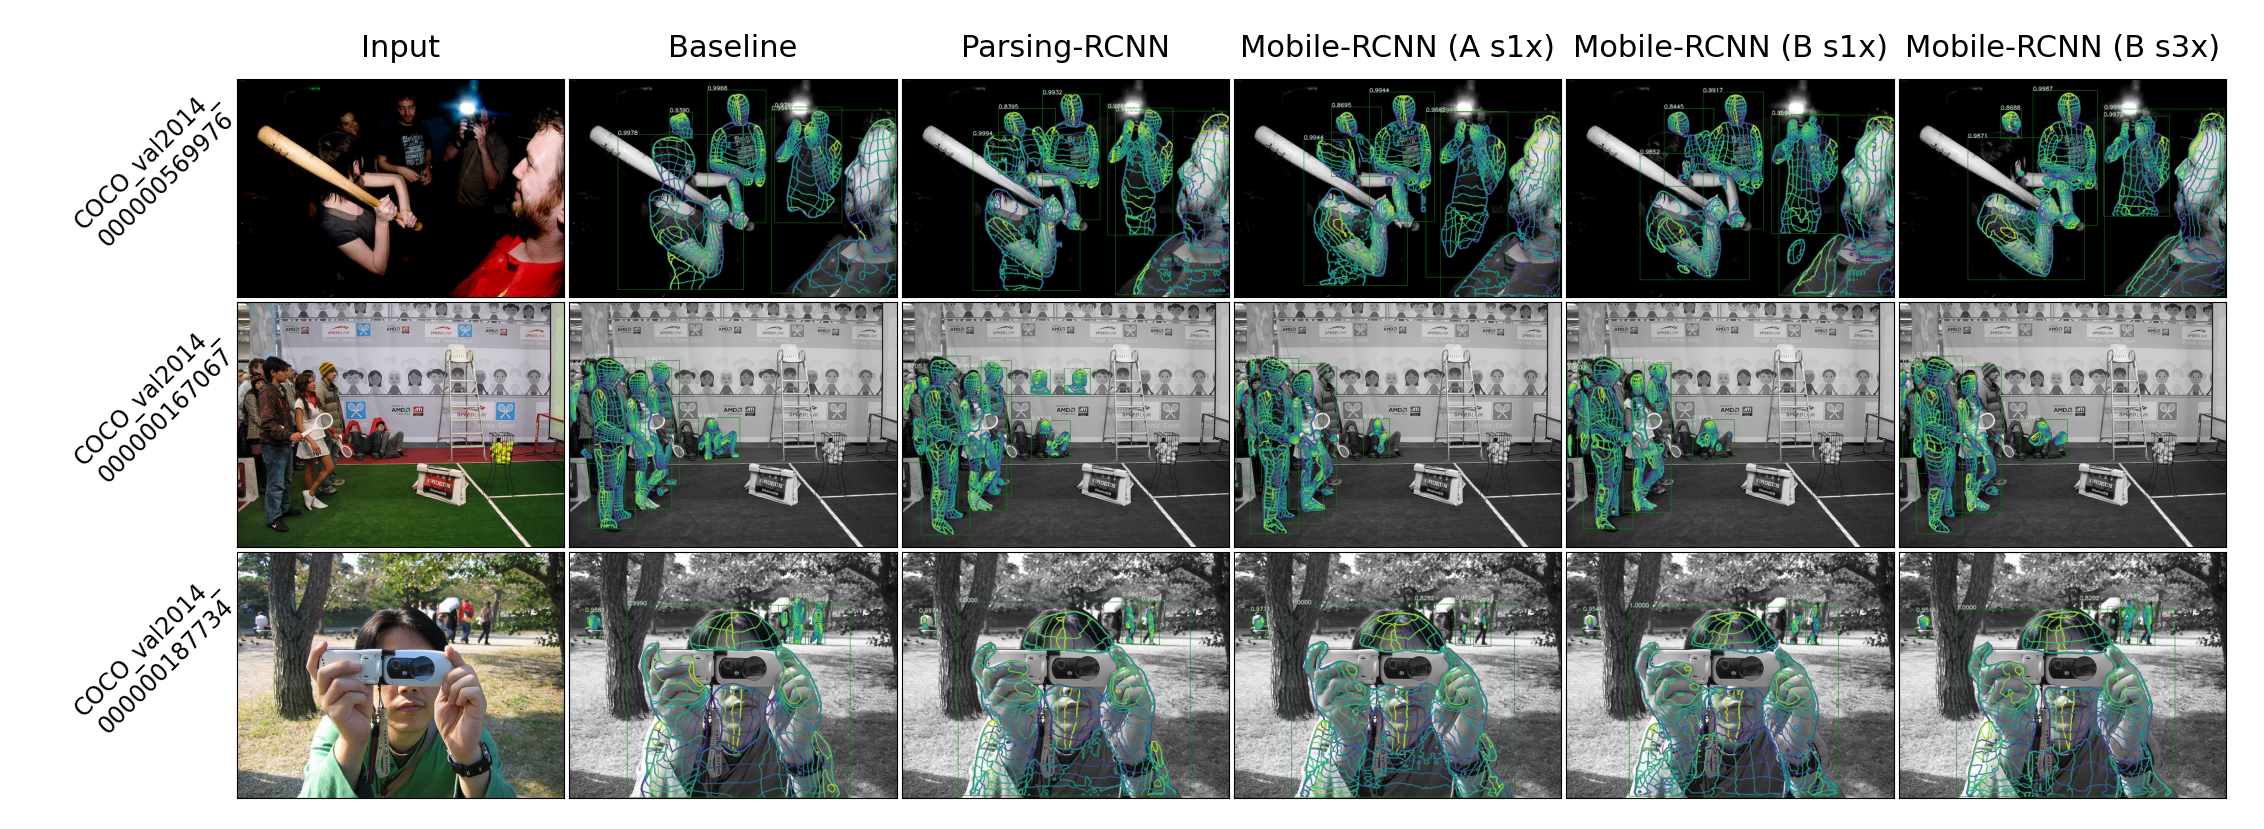
\includegraphics[width=0.9\textwidth]{Figures/densepose/qconfigs_decr.png}
\caption{Qualitative comparison of different models. We depict contours with color-coded U and V coordinates as an output of the model.}
\label{fig:fconfigs}
\end{figure*}

\begin{figure*}[t!]
\centering
\includegraphics[width=0.8\textwidth]{Figures/densepose/mob_comp2.png}
\caption{Qualitative comparison of different backends. We depict contours with color-coded U and V coordinates as an output of the model.}
\label{fig:configs}
\end{figure*}

\subsection{Smartphone-based implementation}


\begin{table*}[t!]
\centering
\resizebox{0.8\textwidth}{!}{
\begin{tabular}{cccccc}
\hline
image shortest side & box AP & dp. AP & GPU FPS & CPU FPS & mobile CPU FPS\\\hline
200px & 36.449 & 19.028 & 27.549 & 10.277 & 2.355\\
400px & 49.181 & 43.916 & 24.648 & 6.921 & 0.954\\
512px & 51.709 & 47.887 & 26.970 & 4.976 & 0.640\\
600px & 53.423 & 49.675 & 25.669 & 4.290 & 0.498\\
800px & 54.744 & 50.560 & 24.033 & 3.046 & N/A\\
1000px & 55.163 & 49.466 & 20.061 & 2.071 & N/A\\\hline
\end{tabular}}
\caption{The impact of image size. Results are obtained with Mobile Parsing R-CNN (B s3x, test-tuned) on DensePose-COCO \textit{minival}. The N/A values correspond to tensor sizes that produced errors on mobile device}
\label{table:pixel}
\end{table*}

\begin{table*}[t!]
\centering
\resizebox{0.9\textwidth}{!}{
\begin{tabular}{ccccccccccc}
\hline
max \# of people & box AP & box APs & box APm & box APl & dp. AP & dp. APm & dp. APl & GPU FPS & CPU FPS & mobile CPU FPS\\\hline
1 & 83.110 & - & 83.389 & 83.173 & 54.329 & 48.203 & 54.765 & 27.508 & 5.859 & 0.684 \\
2 & 74.700 & 24.058 & 56.672 & 77.359 & 52.402 & 47.694 & 52.991 & 27.729 & 5.626 & 0.664 \\
3 & 71.508  & 16.357 & 54.621 & 76.280 & 52.324 & 47.973 & 52.905 & 26.767 & 5.584 & 0.638 \\
4 & 68.818 & 19.532 & 52.693 & 75.693 & 52.050 & 43.131 & 52.838 & 27.198 & 5.510 & 0.606 \\
5 & 66.756 & 20.252 & 53.543 & 74.807 & 51.468 & 44.154 & 52.501 & 27.732 & 5.443 & 0.603 \\\hline
\end{tabular}}
\caption{The impact of number of people in the frame on performance characteristics. Results are obtained with Mobile Parsing R-CNN (B s3x, test-tuned) on DensePose-COCO \textit{minival}. The shortest image side is 512 pixels}
\label{table:people}
\end{table*}

We evaluate the mobile model with Caffe2 runtime, running on a smartphone with ARM processor with 8 cores, 8 threads, and the highest core clock of 2600 MHz.

We use the deployment conversion tools provided by Detectron2 \cite{detectron2}. Specifically, the network is transferred first to ONNX format, then to Caffe2 format.

% \textbf{MODEL.RPN.POST_NMS_TOPK_TEST 100 MODEL.ROI_HEADS.NMS_THRESH_TEST 0.3}
In general, two-stage models introduce numerous hyper-parameters. In case of test-time hyper-parameters, we found empirically, among many different options, that choosing $100$ instead of $1000$ region proposals per \textit{neck} level after non-maximum suppression (NMS) in RPN and changing IoU threshold in NMS from $0.5$ to $0.3$ leads to a significant boost of the model. Therefore later, we use this setup of the model and call it Mobile Parsing R-CNN (B s3x test-tuned).

We check the impact of the image size on the model (see Table~\ref{table:pixel}). The lower resolution of the image, the faster inference we get, but the reduction of image size results in a reduction of densepose AP. In the case of mobile inference, we apply the model on images with the shortest side of size 512 pixels, because it is the lowest resolution processed by the model during the training phase.


% TODO put a number on % of images with less than 5 people 
We are mostly interested in practical applications on the end-device with data fed straight from the device's camera. In this case, usually, the limited number of people appears in the frame. We test the model performance on filtered versions of COCO-DensePose minival partition, where the filtering is based on the maximum number of people in the image. The results can be seen in Table~\ref{table:people}. One can see that the fewer people are in the image, the better performance of the model in AP and FPS. Usually, the fewer people in the image, the more area each person occupies in the frame, which leads to more accurate predictions.

\subsection{Model quantization results}

Here we report the performance statistics of the model obtained using the quantization approach described in Section~\ref{quant}. Thanks to the quantization, we increased the speed of inference by a factor of two and decreased the model size by a factor of three. See exact values in Table~\ref{table:quant}.


\begin{table}[!t]
\centering
\resizebox{0.4\textwidth}{!}{
\begin{tabular}{cccccc}
\hline
weights type & model size & dp. AP & CPU FPS \\\hline
float32 & 13.8mb & 47.887 & 4.976 & \\
int8 & 4.3mb & 44.033 & 8.310 & \\\hline
\end{tabular}}
\caption{The effect of quantization. Results are obtained with Mobile Parsing R-CNN (B s3x, test-tuned) on DensePose-COCO minival. The shortest image side is 512 pixels}
\label{table:quant}
\end{table}
\section{Conclusion}

In this work we showed that it is possible to significantly compress and speed up models ($17\times$ model size reduction and $2\times$ latency improvement) for DensePose estimation task utilizing existing state-of-the-art solutions of this task's subproblems, achieving a good balance between speed, model size and average precision of the model. In the process, we performed an ablation study of 23 different backbones and detection pipeline characteristics, particularly applied for the DensePose task.
By optimizing different parts of R-CNN-like models, we achieved significant performance improvement compared to the baseline model.
We performed deployment of the final model to the mobile device, measured its performance, and discovered factors affecting it. 
The proposed architecture Mobile Parsing R-CNN is both fast and light-weight. Notably, the final model weighs 13.8MB and runs near real-time $\sim27$ FPS on Nvidia Tesla 1080Ti GPU, and $\sim1$ FPS on a mobile device using the only CPU. Using a runtime environment that utilizes mobile GPU or Neural Network acceleration hardware (NPUs), it would be trivial to get near-real-time performance on a mobile phone.
\newline\newline
\noindent\textbf{Acknowledgment.} The authors acknowledge the usage of the Skoltech CDISE HPC cluster Zhores for obtaining the results presented in this paper. This work was supported partially by the Ministry of Education and Science of the Russian Federation (Grant no. 14.756.31.0001).

%\FloatBarrier

% {\small
% \bibliographystyle{ieee_fullname}
% \bibliography{egbib}
% }

% \end{document}

\newpage
% 
%\newcommand{\root}{Chapters/facev1}

\chapter{Getting Off the Internet: Practical Domain Adaptation for Face Recognition}
\label{chapt:wildface}


\section{Motivation}
%face
For face recognition, one important cross-domain scenario is related to using powerful models pretrained on professional photographs for surveillance data. As it has been already mentioned in \sect{face}, large-scale training datasets for face recognition most often include high-quality images that are very different from those captured by surveillance systems. In person re-identification, the domain difference comes mainly from the illumination condition variations between the camera sets (if the difference of the camera positions is put aside). In contrast,  surveillance face recognition implies a complex domain shift caused by a combination of low resolution, compression and illumination conditions. 


In particular, in this chapter we study the unsupervised domain adaptation scenario, where face recognition is trained using an annotated Internet face dataset and an unannotated dataset of faces collected from a surveillance camera network with low image quality. We mostly focus on the recent class of methods that consider domain-adaptation at the image level. We thus investigate how image transformation achieved with recent unsupervised image transformation techniques such as CycleGAN \citep{ZhuPIE17} can be used for face recognition under strong domain shifts. 

We compare and evaluate several strategies, such as transferring test data to the Internet image domain,  transferring training data to the target domain followed by retraining the network. As a baseline, we also compare to adversarial domain adaptation at feature level described in \chapt{gradrev}.% \cite{GaninUAGLLML16}. 

Our comparison suggests that image transformation (without explicit modeling of separate degradation factors) can be used for unsupervised domain adaptation of face recognition. We, however, demonstrate that special care needs to be taken in order to make such domain adaptation work better than baselines, and come up with practical suggestions on how such improvement can be achieved.

%model
% Since the CycleGAN \cite{cyclegan} architecture for image-to-image translation and stylization appeared, domain adaptation has become one of its active fields of application. This approach differs from the feature-level domain adaptation techniques of \cite{LongC0J15} and \cite{tzeng2014deep} or the method presented in the \chapt{gradrev}, because rather than finding deep domain-invariant representations, it works on the pixel level and aims at building mappings between the image domains. Thus the domain adaptation is done in two steps: building a mapping the source domain to target and retraining the predictor on the transferred source data. (Although it is also possible to combine these two steps into one optimization process.)%cycada

% %pedestrians
% For person re-identification, the pixel-level domain adaptation with CycleGAN has been applied in several recent works \cite{} (after the results of the \chapt{gradrev} were published). Some of them consider different datasets as domains, others aim at utilising synthetic re-identification data to improve the results on real data \cite{}. As demonstrated by these works, image-to-image translation may help a lot to overcome the illumination differences between the source and target camera sets. %Still, to the best of our knowledge, there are no works approaching face recognition for surveillance data.

% This chapter demonstrates the performance of the pixel-level domain adaptation approach based on CycleGAN model in the presence of an extreme domain shift between the usual face recognition training data and surveillance data. The considered surveillance data are harvested from $6$ surveillance cameras in the Moscow subway. Two publicly available face recognition datasets of different image quality are considered for the source domain. The approach is compared to several important baselines, including the reverse translation of the target images back to the source domain and the feature-level domain adaptation suggested in this chapter.

%The remainder of the chapter is organized as follows. Image-level domain transfer and face recognition methods are described in \sect{method}.  We define the variants of the training data augmentation compared in this work in \sect{ft}. Then we give the implementation details in \sect{training}. The quantitative comparisons of the described methods and baselines are presented in \sect{results}. Finally, we conclude the work with discussion and summary in \sect{conclusion}.



%\titlerunning{Short form of title}        % if too long for running head



% \begin{abstract}
% Face recognition in real surveillance scenarios is challenging due to the presence of complex degradation factors. At the same time, the easiest-to-collect and the biggest available training data for face recognition come from the Internet, where images and video frames have higher quality, higher resolution, and better lighting. In this work, we study training face recognition systems under such domain shift. We show that CycleGAN technique can be utilized for transferring labeled training data into the target domain of surveillance camera, and that the transferred data can be used to train face recognition in the new domain. We compare this approach to several baselines including the domain transfer in the opposite direction to turn test data directly to the high-quality domain. Our comparison and evaluation allow us to come up with a viable strategy for training face recognition in surveillance data.
% \keywords{face recognition \and surveillance \and domain adaptation}
% % \PACS{PACS code1 \and PACS code2 \and more}
% % \subclass{MSC code1 \and MSC code2 \and more}
% \end{abstract}


%% !TEX root = ../Thesis_main.tex
\chapter{Introduction}

%video surveillance+
%person re-id+
% originates from Multi-Target Multi-Camera Tracking 
%open world / closed world+
%face : verification/identification
%common aspects: detection , processing, recognition
%deep learning

%retrieval
%fine-grained recognition
%adaptation

%datasets (cut from the papers) + table with reid dataset?
%architectures
%definitions?
%contribution - what is done
\section{Context}
\subsection{Problem of 3D reconstruction}

\subsection{Approaches for solving 3D Reconstruction problem}

Solutions for a reconstruction problem can be grouped in two major groups: 1) Geometric approach - when problem is represented as optimisation of scene state given constrains on projections of scene state to data, 2) Machine Learning approach - inverse model is optimisation.

If $X$ - is scene data, $z$ - is the state of the scene, and $g_i(z)$ - projection function of 3D scene $z$ state to perspective $i$, then to find an optimal 3D reconstruction, one solves this minimisation problem:
\begin{equation}
z_{rec} = \min_z\sum_i|X_i-g_i(z)|_2 .
\end{equation}

This approach only solves problem for once scene and does not provide any semantic information about it, only basic geometric information. 
The second approach is more modern and better fitted for machine learning applications, because instead of optimizing state of the scene, it's optimizes a model that performs computation from input data to some semantic (intrinsic) parameters, and can be described as following optimisation procedure:
\begin{equation}
\min_\theta\sum_i|X_i-g_i(f_\theta(\pi))|_2,\ \ \pi=I_\theta(\{X_i\}_i),\ \ z=f_\theta(\pi),
\end{equation}
where $\pi$ - are scene parameters, $f_\theta(\pi)$ - is a generative model that generates 3D state $z$ and it's function is determined by tunable parameters $\theta$.

In reconstruction process information can be introduced in two possible ways: 1) input signal - data measured by some spatial sensor, 2) by adding a priori knowledge while training the Inverse model or by design choice of reconstruction algprithm. Between the two source exist a fundamental trade-off and detirmination of which is dominant can be quite difficult \cite{tatarchenko2019single}.


\subsection{Objectives and Motivations}

The goal of this work to improve methods of 3D reconstruction in holistic context using deep learning systems. For efficient applications such as robotics in human environments and mixed reality more advanced machine perception systems are needed. Human perception is a complex system with several properties not all of which are replicated in modern machine perception systems. From cognitive sciences it's known that ability to model environments is one of the most important for perception system, in area of computer vision this is known as an ability to perform \textit{3D reconstruction} of scenes and environments. To solve this problem in a general case requires application of machine learning.

In particular, the development of such holistic deep 3D reconstruction system includes several important tasks:

\begin{itemize}
􏰀    \item Capturing scenes, complete with colour and depth data of a sufficient quality,
    \item Recalling objects from large scale database of objects,
    \item Segmenting variety of most common elements from sensor data, such as household objects and architectural components,
    \item Detecting and reconstructing shape and pose of and human bodies.
\end{itemize}

Each of these sub-tasks constitutes a challenge in the context of human perception.

The presence of noise in sensor data (e.g., consumer grade depth cameras) is a serious problem for all downstream sub-tasks, low fidelity of this data causes a considerable compaunding performance drop.

\subsection{3D data representations}

We can describe a 3D object in multiple ways, and codification of it's properties has ramifications about capturing different information about objects and scenes, as well as kinds of models that can regenerate them or computational resources needed to process it.
Each representation has it's own pros and cons. We assume 3D information representation to be positive effective and usefull if it captures more relevant information with less storage requirement (compression), increases signal to noise ratio of data, captures shape and texture properties with minimum trade-off.

Here are some popular examples of 3D data representations:
\begin{enumerate}
	\item Multiple 2D projections - captures surface texture, highly redundant representation if images overlap, also vulnerable to optic illusions.
	\item Voxels - simple, most of the time can be sparse, represents rough volumetric properties vell but losses most of surface properties.
	\item Point Cloud - are sparse in a sense that they don't capture empty space, losing all surface properties besides color and estimated normals and most of volumetric properties.
	\item 2.5D (RGB-D) images are widespread because of cheap measurement devices, capture volumentric depth but succeptable to occlusion of bodies in a scene and records a lot of noise with actual signal.
\end{enumerate}



%Motivation: RGB-D scanning is here and we want to have a fine-grained understanding of the 3D captures
In the recent years, a wide variety of consumer-grade RGB-D sensors, such as the Intel Real Sense, Microsoft Kinect, depth-sensor enabled smartphones, enabled inexpensive and rapid RGB-D data acquisition. Increasing availability of large, labeled datasets (e.g.,~\cite{chang2017matterport3d,dai2017scannet})  made possible development of deep learning methods for 3D object classification and semantic segmentation. At the same time, acquired 3D data is often incomplete and noisy; while one can identify and segment the objects in the scene, reconstructing high-quality geometry of objects remains a challenging problem.  

An example of the new approach in recent work 
\cite{avetisyan2019scan2cad}, uses a large dataset of clean, labeled geometric shapes
\cite{chang2015shapenet}, for classification/segmentation associating the input point or voxel data with object labels from the dataset, along with adapting geometry to 3D data.  This approach ensures that the output geometry has high quality, and is robust with respect to noise and missing data in the input.  
At the same time, a ``flat'' classification/segmentation approach, with each object in the database corresponding to a separate label and matched to a subpart of the input data corresponding to the whole object, does not scale well as the number of classes grows and often runs into difficulties in the cases of extreme occlusion (only a relatively small part of an object is visible). 
Significant improvements can be achieved by considering object \emph{parts}, or more generally part hierarchies. 
Part-based segmentation of 3D datasets promises to offer a significant improvement both in finding the best matching shape in the dataset, recognizing objects from  highly incomplete data (e.g., from a couple of parts) from  as well as more precise geometry adaptation as well as, potentially, assembly of new shapes out of existing parts yielding a closer match to the input data. 

large collection of 3D models in database can be reduced to structured representations, 
objects with occluded sub-parts still can be recognized by parts available in the scan and the rest can be guessed with high probability, using parts, we can reconstruct new objects that are not yet present in the database of shapes.

Based on different approaches for volumetric information integration, from enhancements of  methods such as volumetric fusion \cite{curless1996volumetric}, to probabilistic  methods, and plethora of methods based on their combinations.

Compared to computer graphics models manually created by 3D professionals, 3D scans are noisy and incomplete.
Amount of noise and limited resolution of consumer-grade scanning hardware pose significant challenges for solving this important problem of scene reconstruction. 
Approaches of reconstruction based on fitting existing 3D assets into scene scans, have shown a lot of promise but still had problems with finding exact models from large database such as ShapeNet \cite{chang2015shapenet}, because of occlusion and lack of spatial context.

Learning-based approaches are very good at extracting features representative of objects and scenes as a whole, allowing to fill in occluded areas or guess parts affected by noise \cite{dai2017shape,dai2018scancomplete,song2017semantic}. These features are sufficient for scene completion, but they are not as good at recovering geometric primitives like: sharp edges, planar surfaces or borders between sub-parts, resulting in reconstruction quality much poorer than that of 3D content created by humans.

In this work, we focus on the key problem of semantic part segmentation of objects in the scenes, enabling further improvements in  dataset-based reconstruction. 
Semantic part-segmentation, can help in these situations, when sufficient number of the object parts is visible model can infer the non-visible parts essentially completing an object in sense of maximum probability conditioned on input data.

In human-made environments, a lot of objects have naturally defined semantic sub-parts, and those sub-parts can, in turn, have their sub-parts, i.e., parts form \emph{hierarchies}.  In our work, we use scene and object representation based on such part hierarchies.  We show how a part-labeled dataset of scanned 3D data suitable for machine learning applications can be constructed, and used to improve the performance of segmentation algorithms. 

Definitions of sub-parts are based on a set of primitive elements that were manufactured by one formation method or from one material.

Because of that and the fact that static scenes have other relationships between objects (fixed to each other or in direct surface contact), it's reasonable to suggest a scene description format that possesses a property of hierarchy (e.g., trees or other kinds of graphs).
Representing scenes as a discrete structures with multiple relationships between nodes. Such relationships like composability of its parts and affordances between whole objects, in turn allowing to compose a scene from separate objects.

\todo{merge these paragraphs}

In domain of human-made environments a lot of objects have sub-parts and those sub-parts can in turn have their own sub-parts. Definition of sub-part is often based on a set of primitive elements that were manufactured by one formation method or from one material. Because of that and the fact that static scenes have other relationships between objects (fixed to each other or in direct surface contact), it's reasonable to suggest a scene description format that possess a property of hierarchy (e.g. trees or other subgraphs).
A lot of researchers over the last 20 years came to the same conclusion. A lot of work on that problem was done by Mumford and Zhu in \cite{zhu2006stochastic}.

One of the papers dealt with problem of modeling Images as a hierarchy of super-pixels. \cite{russell2009associative}, or as a tree of geometric primitives (e.g. cylinders, spheres or 3D boxes) \cite{li2017grass}.

% point cloud (PC) turned in to a graph (based on proximity) point-cloud parser network reduces number of nodes and edges and enriches their feature vectors. First part of the decoder network functions similar to Feature Pyramid Network in CNNs, which performs local computations on different scales, followed by "pooling or convolutions" with reduced spatial component and increased feature components, thus leaving only small number of "keypoints" required to outline shapes of objects.



CAD constructor network translates that graph into CAD object (tree with primitives and combination rules). CAD rendered makes a mesh out of that object thus a residual between original PC and Mesh can be calculated.

Proximity Graphs - concept that allows to build a bridge between Point Clouds and Graph Processing. This area of computational geometry has a lot of theoretical results to offer for Deep Learning piplene designer.


\subsection{Definitions and examples}
\subsection{Data sources and devices}

\section{Inverse Graphics Problem formulation}

\cite{rezende2016unsupervised,eslami2016attend,kulkarni2015deep,wu20153d,izadinia2017im2cad}

Inverse graphics approach enables to solve a problem of "real-world" scene understanding through reconstruction of that scene and comparison it to measured data in some form.

Because it's a fairly new method it has some unexplored facets:
\begin{enumerate}
    \item How can we scale to hundreds and thousands of objects with different parameters.
    \item Embedded representations better than procedural generation
    \item Are there format that can have all advantages of CAD models and probabilistic properties that arise from real-world uncertainties.
\end{enumerate}

Central goals of computational perception is to get structured description of scenes from measurements such as photographic images, scans and videos.

Computer Vision as Inverse Graphics is the most rational formulations that could help us achieve this goal.

In the past, it has been hard to directly solve these problems in practice because of computational limitations.

However, it may be right time to take another look at this idea due to significant advances in deep learning for computer vision, probabilistic programming, and computer graphics.

Probabilistic programming - a tool that allows us to implement complex models while keeping ability to perform inference, extend with other probabilistic models by being general-purpose.

Re-formalizing inverse graphics in terms of probabilistic programming and deep learning allow us to solve even more complicated vision problems with off-the-shelf computational technology.

To make this approach scalable, my research can incorporate effective techniques such as: approximate Bayesian computation, differentiable programming for rendering.

Computer Graphics nowadays seems to be improving at a great pace in terms of designing solutions for hard image synthesis problems, but these solutions are usually hand-made and not flexible enough to cover all needs for general-purpose real world object generating, latest advances in generative models can help with that.


\subsection{Overcoming lack of information}

\section{Datasets}

Only recently research community started accumuulating sugnifficant amount of algined sensor data to solve large scale 3D reconstruction problems in deep learning context. In last 4 years we saw an explosion of 3D shape databases and 2D-to-3D indoor scene datasets, such as ShapeNet, 2D-3D Semantic, Scannet and Matterport3D datasets. Because accuracy and reacall properties of deep learning models scale with amount and variety of data, number of state-of-the-art models grew as well.

\section{Architectures}

PanopticFusion~\cite{narita2019panopticfusion} is a model that is able to segment large indoor scenes and separate \textit{Stuff} and \textit{Things}.


For outdoor datasets Point Cloud representation of data is more common because of large empty spaces and the way LiDAR sensor collects data. In such setting instance segmentation is nessesary first step for reconstruction~\cite{zhang2020instance}.

\subsection{Multi-view models}

Detailed comparision of multi-view 2D CNN model and 3D volumetric CNN can be found in \cite{qi2016volumetric}.

\subsection{Implicit 2D models}

Like inverse graphics network. Model takes 2D images and returns 2D images with 3D properties changed. 

\subsection{3D convolutional models}

Model generates or processes voxel image with 3D convolutional operation implemented Dense or Sparse.

Semantic information can boost the reconstruction performance because deep learning systems are able to pick up onto consistent signal \cite{jiao2018look,tatarchenko2019single,kendall2018multi}.

\subsection{2D to 3D Projection models}

Model uses camera parameters to compute 3D representation using 2D/2.5D images and projection operation.

\subsection{Point Set layers}

Neural Network processes a set of points to classify, segment or predict new set of points.

\subsection{Graph-Convolutional layers}

Model processes Geometric Graph where nodes represent points registered on a surface of objects or parts of objects, and has geometric or other information representing edges between points. Layers process activations associated with nodes taking into account the connectivity.

\subsection{Differentiable rendering layers}

Rendering operation is implemented in a differentiable way, allowing backpropogation of gradient information from 2D images to meshes and textures of the objects being rendered.

\subsection{Mesh generating layers}

Neaural Network layers that can create a mesh by way of processing a template 3D shape with parametracised operation or meshing other 3D shape representation generated by computation from weights and input.

\subsection{Implicit 3D models}

Models like NeRF, PIFU3D, neural network implements a rendering function depending on view angle and other graphics parameters, one model represents one scene and don't generalise for viriety of scene inputs.



\section{Contributions}

% \chapt{hist}, \chapt{bilinear} and \chapt{gradrev} use  person re-identification architecture of \citep{Yi14} as a baseline method (it is also  described in \sect{intro_architectures}).  \chapt{bilinear} is based on the results of \chapt{hist}: the loss function introduced in \chapt{hist} is used for 
% all the experiments in \chapt{bilinear} as it was demonstrated to show the best performance for person re-identification. 
% The results of \chapt{gradrev} were chronologically the earliest among all the results presented in this work, therefore  methods  from \chapt{hist} and \chapt{bilinear} were not used there. 
% Although the contributions of each of the chapters are independent, they are all parts of building a person re-identification pipeline and can be applied simultaneously. 
% \chapt{wildface} considers domain adaptation for surveillance face recognition and uses the method from \chapt{gradrev} as one of the baselines.
 


 \begin{figure}
 \centering
    \includegraphics[height=0.7\paperheight]{Chapters/face/da_picture_vertical_TS.pdf}
    \caption{The overall scheme of the two possible approaches to the face recognition problem considered in our work. Surveillance and Internet image domains are denoted with green and blue rectangles correspondingly (the data examples are taken from our surveillance dataset and the YouTube faces dataset).
    The \textit{face restoration} approach (blue lines) transfers the surveillance data images to the Internet domain using the transform $F^{T \rightarrow S}$. It then uses the ``blue'' face recognition model trained on annotated internet images to compute descriptors for the transfered images. Meanwhile, the \textit{domain adaptation} approach (green lines) transfers the annotated internet data to the surveillance domain, and then uses the transfered data to train the ``green'' face recognition model, which is then applied to unannotated surveillance images. Our work evaluates and compares several variants of both approaches.}
  \end{figure}

  
%\section{Related work}
\label{sect:related}

There are two main research directions dedicated to face recognition for low-quality data: (i) the face restoration approach and (ii) the domain adaptation approach. In the face restoration-based approach, low-quality images are enhanced and restored to facilitate recognition. The ability to reuse existing recognition systems that were developed for high-quality data comes as a natural benefit of such methods. Domain adaptation methods are conversely aimed to change the existing recognition systems so that they are better suited for the target domain (i.e.\ low resolution/quality images). We now provide a brief review of both approaches.

\subsection{Face restoration methods}

There is a vast range of methods that perform face restoration. In most of them, different degradation types are considered separately. Pan \textit{et al.} \cite{pan2014deblurring} propose an effective face deblurring method based on approximating blur kernel followed by non-blind deconvolution. The blur kernel  approximation is guided by the known non-blurred exemplar with the structure similar to the input image structure. 

In Zhang \textit{et al.}~\cite{ZhangYZNH11}, deblurring and recognition tasks are considered simultaneously. They use a sparse representation of the input image in terms of the gallery image set. The blur kernel and representation coefficients are estimated iteratively. Classification is finally performed based on the classes with the highest coefficients in the sparse representation.  


A number of recent methods \cite{TuzelTH16,ZhuLLT16,xu2017learning,huang2017wavelet} explore the task of restoration of extremely low-resolution images using deep neural networks. All these works utilize the paired (aligned) learning scheme, where the high-resolution ground truth is known for every low-resolution image in the training set. The low-resolution training data are simulated using synthetic degradation of the initial high-resolution images. In \cite{xu2017learning} and \cite{TuzelTH16}, a generative adversarial network~(GAN)~\cite{goodfellow2014generative} is used to force the restoration network to produce more natural images. In \cite{huang2017wavelet}, an additional structure-based loss that uses wavelet transform is suggested for the same goal. While the results of these methods are impressive, there is no direct way to use the paired learning approaches for the arbitrary combination of degradation factors that one may encounter when analyzing real images captured by surveillance cameras. 

\subsection{Domain adaptation methods}

Several recent works are dedicated to domain adaptation in the context of different recognition tasks \cite{Volpi_2018_CVPR,Hong_2018_CVPR,Deng_2018_CVPR,Bousmalis_2017_CVPR,Murez_2018_CVPR}. In \cite{Murez_2018_CVPR}, 
\cite{Bousmalis_2017_CVPR} and \cite{Deng_2018_CVPR}, image-level domain adaptation is performed for segmentation, classification and similarity learning (person re-identification) correspondingly. Hong \textit{et al.} \cite{Hong_2018_CVPR} and Volpi \textit{et al.} \cite{Volpi_2018_CVPR} resort to feature-level domain adaptation for segmentation and classfication tasks. Both feature-level and image-level techniques are used in \cite{Hoffman17}.

Some of the aforementioned methods \cite{Hoffman17,Deng_2018_CVPR,Murez_2018_CVPR} employ CycleGAN framework  to change the domain of training data for classification, segmentation, and person re-identification. Here we explore a similar approach for the task of face recognition in the presence of complex degradation factors.

Hong \textit{et al.} \cite{HongIRY17} and
Sohn \textit{et al.} \cite{SohnLZY0C17} approach face recognition tasks for low-quality image domain. They consider image degradation as a domain shift and perform feature-level unsupervised domain adaptation based on adversarial learning showing better recognition results. 
The works \cite{HongIRY17} and \cite{SohnLZY0C17} are very related to ours: the authors show that domain-specific data augmentation is essential for training face recognition systems. 
 However, in both works, the data augmentation is performed 'by hand' (the degradation types and hyper-parameters for transforms are chosen and fixed), while we augment the training data in an automatic manner utilizing the CycleGAN framework, which can also be viewed as an image-level domain adaptation.
%Additionally, in contrast to \cite{HongIRY17}, we do not consider extremely large pose variation. Instead, we are more focused on the image degradation factors (e.g. the combination of small size, blur, JPEG-compression). 
Differently from \cite{SohnLZY0C17}, where evaluation is performed for the Youtube faces dataset, we approach the task in the presence of the somewhat stronger domain shift, as our test data are captured by surveillance cameras and are mostly of much lower quality.




%Some works already successfully use CycleGAN technique to perform an unsupervised domain adaptation. \cite{CYCADA} approached semantic segmentation. % add avput CYCADA

%recognition and reconstruction approaches
% Several existing works consider restoration and recognition problems jointly. In some works, authors apply the recognition-based priors to achieve better restoration results. \cite{TODO , Xu} 

% There are also approaches jointly performing explicit recognition and restoration
% In \cite{TODO Close  the  loop:  Jointblind  image  restoration  and  recognition  with sparse representation prior , Baker} The  proposed  approaches  perform  recognition  using  a  limited  number  of  gallery  images.   In parallel, they reconstruct the input image and classify it based on labels of the most relevant examples found in the train set.

 
% One of the baselines used in this work applies the similar scheme: CycleGAN framework is used to transfer the low-quality test data into the high-quality domain, the domain classifier serves as 'restoration' loss. We additionally introduce the recognition component into this scheme: another baseline is the same CycleGAN but with domain classifier based that is learned using features calculated with the pre-trained face recognition network.




    \begin{figure}
    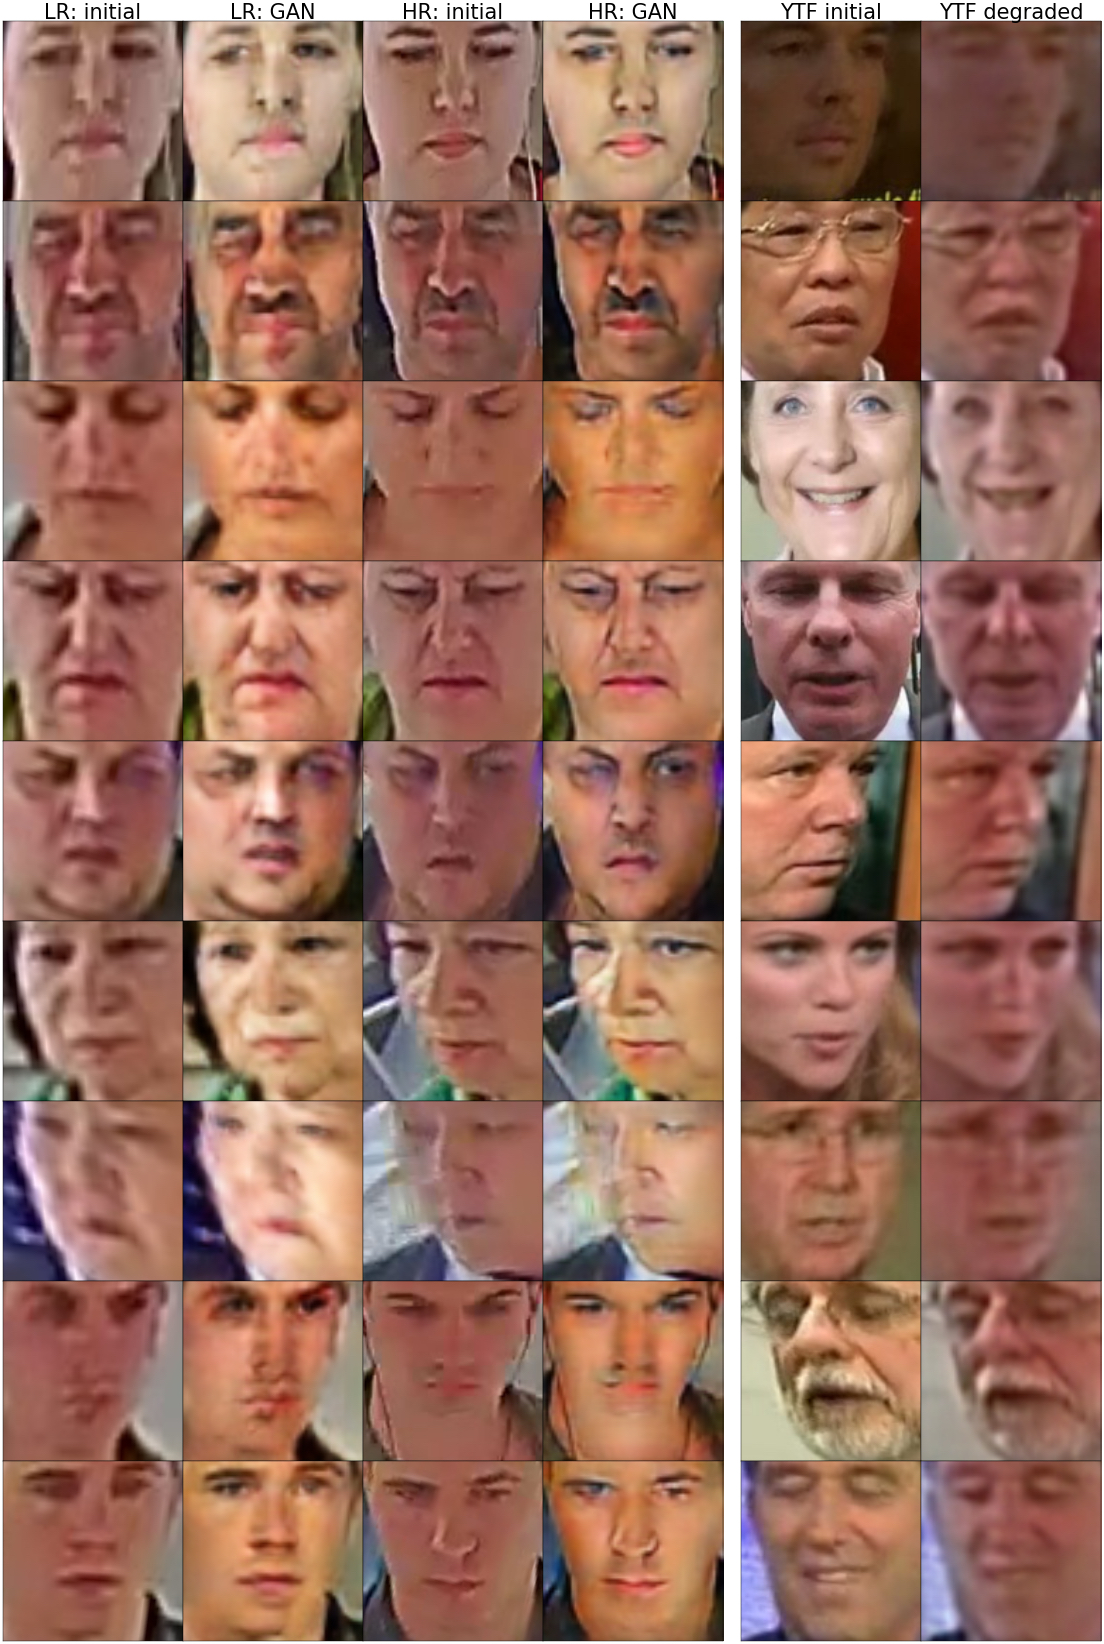
\includegraphics[width=\linewidth]{Chapters/face/Fig2.jpg}
    \caption{Columns one and three show images from our test surveillance data, while columns two and four contain the corresponding images transformed to the Internet data domain. See section \ref{sect:method} for the details. The last two columns show the examples of the reverse transformation from the Internet image domain to the surveillance image domain for the YouTube faces dataset.  }\label{fig:lr_hr_gan_res_ytube_initial_degraded}
  \end{figure}
  
  
\section{Evaluated approaches}
\label{sect:method}
\bigskip
\indent\textbf{Face recognition for the low-quality image domain}\\
%\subsubsection{Face recognition for the low-quality image domain}
\label{sect:strategies}
In this work we consider and compare two main approaches to face recognition for surveillance data: 1) restoration-based approach and 2) domain adaptation of existing face recognition neural networks. 

We consider two facial image domains: \begin{itemize}
\item domain $T: \{X^{T}_{i} \}_{i=0}^{N_T}$ that includes low-quality facial images $X^{T}_{i}$ captured using surveillance cameras. Usually, there are no identity labels provided, as assigning identity labels is quite challenging and may not even be feasible.
\item domain $S: \{(X^{S}_{i}, Y^{S}_{i})\}_{i=0}^{N_S}$ that includes facial images $X^{S}_{i}$ harvested from the Internet. These images are usually of higher quality and are taken in good lighting conditions. We assume that the data in this domain are supplied with identity labels $Y_i$.
\end{itemize}  

According to the available labeling, we can consider two different pipelines for building face recognition systems for surveillance data. The first option is the restoration-based approach when we use transform $F^{T \rightarrow S}: T \longrightarrow S$ as a face restoration method and then apply existing recognition neural network $R^{S}$ that is pre-trained on images from the domain $S$. The second option is to use the transform $F^{S \rightarrow T}: S \longrightarrow T$ to transfer the large collections of labeled training data to the target domain of surveillance images. In this scenario, we retrain the existing face recognition networks resulting in the new adapted model $R^{T}$.

More formally, we consider the following two pipelines for face recognition in the domain $T$.  We denote $d^{T}$ and $d^{S}$ the descriptors produced by the domain-specific face recognition models $R^{T}$ and $R^{S}$. These descriptors may be used e.g.\ to identify matching and non-matching faces based on the distances between them. 
 
$F^{T \rightarrow S}: T \longrightarrow S$ and $F^{S \rightarrow T}: B \longrightarrow A$ are the image-level domain transfer mappings. In the restoration-based approach, we train the recognition model $R^{S}$ using labeled data  $\{(X^{S}_{i}, Y^{S}_{i})\}$ where $X^{S}_{i} \subseteq B$. We then test the learned model by computing the descriptors $d^{S}$ after applying the network $F^{T \rightarrow S}$:  $d^{S} = R^{S}(X^{T\rightarrow S}) = R^{S}(F^{T \rightarrow S}(X^{T}))$

In the domain adaptation approach, we train the recognition network $R^{T}$ using labeled data $\{(X^{S \rightarrow T}_{i}, Y^{S}_{i})\}$, where the training examples $X^{S \rightarrow T }_{i} = F^{S \rightarrow T}(X^{S}_i)$, $X^{S}_i \subseteq S$ are obtained by transforming the high-quality images to the low-quality domain using the learned transformation $F^{S \rightarrow T}$. In this case, we apply the learned network directly to the low-quality images by computing and working with their descriptors $d^{T} = R^{T}(X^{T})$. The two approaches are compared below.


%image describing train and test time for both schemes
\bigskip
\indent\textbf{Learning domain transfer mappings}\\
%\subsubsection{Learning domain transfer mappings}
\label{sect:domain_transfer}
We use the CycleGAN approach~\citep{ZhuPIE17} to simultaneously learn the domain transfer mappings in both directions: $ F^{T \rightarrow S}: T  \longrightarrow S$ (restoration-based approach) and  $F^{S \rightarrow T}: S \longrightarrow T$ (domain adaptation approach). Here we describe the objective functions used for learning the domain transfer architecture.

We use the variant of CycleGAN similar to the one introduced in \citep{LiuNIPS2017} as we found it resulting in more stable and visually more plausible results for our task than the original framework \citep{ZhuPIE17}. Following \citep{LiuNIPS2017}, we decompose the domain transfer mappings into the compositions of encoders and generators: $F^{T \rightarrow S} = G^{S} \odot E^{T} $ and $F^{S \rightarrow T} = G^{T} \odot E^{S} $. Here, the encoders $E^{T}$ and $E^{S}$ transfer input images to the latent space, and generators $G^{S}$ and $G^{T}$ map the input latent codes to the domains $S$ and $T$.
 
For inputs $X^{T} \subseteq T $ and $X^{S} \subseteq S $ the results of their transfer to the opposite domain will be:
\begin{equation}
    X^{T \rightarrow S} = F^{T \rightarrow S}(X^{T}; \theta^{T}_F) = G^{S}(E^{T}(X^{T}))  
\end{equation}
\begin{equation}
    X^{S \rightarrow T} = F^{S \rightarrow T}(X^{S}; \theta^{S}_F) = G^{T}(E^{S}(X^{S}))
\end{equation}

The objective function used by the CycleGAN approach for learning is composed of the two symmetric parts:
\begin{equation}
\mathcal{L} = \mathcal{L}^{T} + \mathcal{L}^{S},
\end{equation} where $\mathcal{L}^{T}$ further decomposes as:
\begin{equation}\label{eq:domain_loss}
     \mathcal{L}^{T} = \mathcal{L}_{\text{GAN}}^T + \lambda_1 \mathcal{L}_{\text{cycle}}^T + \lambda_2 \mathcal{L}_{\text{rec}}^T,
\end{equation}
while $\mathcal{L}^{S}$ has same structure as $\mathcal{L}^{T}$:
\begin{equation}\label{eq:domain_loss2}
     \mathcal{L}^{S} = \mathcal{L}_{\text{GAN}}^S + \lambda_1 \mathcal{L}_{\text{cycle}}^S + \lambda_2 \mathcal{L}_{\text{rec}}^S,
\end{equation}


We now describe each of the terms in \eq{domain_loss}.
The GAN loss serves as the optimization objective for the domain transfer: 

\begin{dmath}
\mathcal{L}_{\text{GAN}}^A = 
    \min_{\theta^{S}_F} \max_{\theta^{T}_D} \mathbb{E}_{x \sim p_{X^{T}}} \log D^{T}(x) +
    \mathbb{E}_{x \sim p_{X^{S}}} \log \big(1 - D^{T}(F^{S \rightarrow T}(x)) \big)\,
\end{dmath}


Here, $D^{T}(X;\theta^{T}_D)$ and $D^{S}(X;\theta^{S}_D)$ are discriminators for the domains $T$ and $S$ that are trained in parallel with the training of the domain transforms.

The other two terms are the so-called cycle consistency loss: 
\begin{equation}
\mathcal{L}_{\text{cycle}}^T = L_1(F^{S \rightarrow T}(F^{T \rightarrow S}(X^{T})), X^{T})  
\end{equation}
and the reconstruction loss:
\begin{equation}
\mathcal{L}_{\text{rec}}^T = L_1(G^{T}(E^{T}(X^{T})), X^{T}) 
\end{equation}
In both terms, $L_1(\cdot,\cdot)$ denotes the $L_1$ distance.

We show the results of transferring the Internet and surveillance images to the other domain in figure \ref{fig:lr_hr_gan_res_ytube_initial_degraded}. While these results look interesting, we do not analyze their visual quality, as we are ultimately interested in the recognition performance rather than obtained visually-convincing images.

\bigskip
\indent\textbf{Learning face recognition models}\\
%\subsubsection{Learning face recognition models}
\label{sect:face_recognition}
In both scenarios that we compare in this paper, we need to train a face recognition model that turns images into vectorial descriptors. This happens either in domain $S$ (in the face restoration approach) or in domain $T$ (in the domain adaptation approach).

In either case, the goal of the training is to build a deep convolutional network that converts face images to the descriptors, such that matching face images have close descriptors and non-matching face descriptors have dissimilar descriptors. We use the Binomial Deviance loss~\citep{Yi14} to perform such training \eq{bindev}. We note that the choice of a particular metric learning loss is orthogonal to our study.

Alternatively to the models trained using the setting discussed above, we also consider reusing the VGG face model trained by the authors of~\citep{parkhi2015deep} on the VGG-face dataset.


 
\section{Experiments}
\label{sect:experiments}

We now perform evaluation and the comparison of the two approaches and their variants. 

\bigskip\indent\textbf{Datasets and protocols} 

\label{sect:datasets}
\bigskip\indent\textbf{Surveillance data}\\
\label{sect:surveillance}
For the surveillance image domain ($A$, as denoted in \sect{strategies}), we have obtained a surveillance dataset comprising faces from five cameras in Moscow subway. Our dataset consists of two subsets of images, denoted as \texttt{LR} (low-resolution) and \texttt{HR} (high-resolution) according to their size in pixels. Sizes are calculated as the face bounding box heights. Mean face heights for \texttt{LR} and \texttt{HR} subsets were $49.72$ and $106.19$ pixels correspondingly. The \texttt{LR} images range from $37$ to $63$ pixels, and \texttt{HR} images from $75$ to $224$. The DLib \citep{dlib09} library was used for face detection and subsequent alignment. 
 
Generally, the identities of people occurring in the video are unknown, and therefore we mine matching faces in the dataset by considering temporal tracks in videos. We assume that face images from different tracks are non-matching. The matching pairs then correspond to pairs of faces from the same track, such that one image belongs to the LR subset and the other belongs to the HR subset. Columns 1 and 3 in \fig{lr_hr_gan_res_ytube_initial_degraded} show some examples of matched pairs. Usually, the quality of face images increases when the person approaches the camera, and therefore \texttt{HR}-subset images are often (but not always) visually better than those present in the \texttt{LR} subset. The division into \texttt{LR} and \texttt{HR} subsets is introduced to ensure that the matched pairs of frames correspond to distinct frames of the temporal tracks. We stress that the mined matching pairs are used for evaluation (testing) only and are not used for training of any networks in our experiments.

We use $96$ identities that are present in both \texttt{LR} and \texttt{HR} for parameter validation and $279$ identities for test. For each of the test identity, there is a pair of matching tracks (one LR track and one HR track). The goal of algorithms is then to build descriptors that would be similar for frames coming from the HR and the LR tracks of the same identity, and would be dissimilar for the HR and the LR tracks corresponding to different identities. Overall, $3,891$ images were used for test.

$4,979$ images of identities not present in the test set are used for training the unsupervised domain transfer described in \sect{domain_transfer} (tracking-based information was not used to train the ConvNets). The mean number of frames for each identity in \texttt{LR} and \texttt{HR} test data are $18.62$ and $17.72$ correspondingly.
 
 
  To evaluate the recognition quality, we match identities across the \texttt{LR} and \texttt{HR} in the following way: we calculate the cosine similarity between the frame set $t_{id_1}^{LR}$ of identity $id_1$ and the frame set, $t_{id_2}^{HR}$ of identity $id_2$ by averaging the similarities of each pair of frames: 

 \begin{align}
     S \left(t_{id_1}^{LR},t_{id_2}^{HR}\right) = \frac {1} { |t_{id_1}^{LR}|*|t_{id_2}^{HR}|}\sum_{i=0, j= 0}^{|t_{id_1}^{LR}|, |t_{id_2}^{HR}|} S \left(f_{id_1,i}^{LR},f_{id_2,j}^{LR} \right), \\
     S\left((f_{id_1,i}^{LR},f_{id_2,j}^{LR}\right) =  cos\left(d_{id_1,i}^{LR},d_{id_2,j}^{LR}\right),
 \end{align}
 where $d_{id_1,i}^{LR}$,$d_{id_2,j}^{HR}$ are the descriptors of the corresponding frames calculated by face recognition neural network $R$ \ref{sect:face_recognition}.
%f_{id_1,i}^{low} \subseteq t_{id_1}^{low} , %f_{id_2,j}^{low} \subseteq t_{id_1}^{low}

% To evaluate the recognition quality, we match identities across the \texttt{LR} and \texttt{HR} in the following way: we calculate the cosine similarity between the frame set $t_{id_1}^{LR}$ of identity $id_1$ and the frame set, $t_{id_2}^{HR}$ of identity $id_2$ by averaging the similarities of each pair of frames: 

% \begin{align}
%     S(t_{id_1}^{LR},t_{id_2}^{HR}) = \sum_{i=0, j= 0}^{|t_{id_1}^{LR}|, |t_{id_2}^{HR}|} S(f_{id_1,i}^{LR},f_{id_2,j}^{LR} ), \\
%     S(f_{id_1,i}^{LR},f_{id_2,j}^{LR} ) =  cos(d_{id_1,i}^{LR},d_{id_2,j}^{LR}),
% \end{align}
% where $d_{id_1,i}^{LR}$,$d_{id_2,j}^{HR}$ are the descriptors of the corresponding frames calculated by face recognition neural network $R$ \ref{sect:face_recognition}.
%f_{id_1,i}^{low} \subseteq t_{id_1}^{low} , f_{id_2,j}^{low} \subseteq t_{id_1}^{low}

\bigskip\indent\textbf{Evaluation metrics}\\

We focus our evaluation on the surveillance data domain. As already mentioned above, during evaluation, we compare pairs of \textit{tracks}, where the first track comes from the \texttt{LR} subset and the second track comes from the \texttt{HR} subset. 

When comparing the two tracks using the recognition metrics, we match all possible pairs of frames and compute the mean average cosine similarity between the computed descriptors over all pairs (more sophisticated schemes involving minimal pairs did not result in better performance). Depending on whether the mean average cosine similarity is higher or lower than a certain threshold $\tau$, we treat a certain pair of tracks as matching or non-matching.

By considering various $\tau$, we then compute the \textit{ROC curve}, the area under the ROC curve (ROC AUC), the $100$\% - EER (Equal Error Rate) statistics, and the average precision (AP) metrics. 



\bigskip\indent\textbf{Internet data}\\
For the Internet image domain ($B$, as denoted in \sect{strategies}) we use three face recognition datasets: Celeb-A \citep{liu2015faceattributes}, YouTube Faces (YTF) \citep{WolfHM11} and the VGG Face datasets \citep{parkhi2015deep}.

The Celeb-A dataset~\citep{liu2015faceattributes} consists of $202,599$ images of high quality and is used for training CycleGAN-based  domain transfer described in \sect{domain_transfer}. 

The Youtube Faces (YTF) dataset~\citep{WolfHM11} and the VGG Face dataset~\citep{parkhi2015deep} are used for the finetuning of the face recognition neural network as described in \sect{face_recognition}. YTF consists of $3,425$ videos of $1,595$
people collected from YouTube, with an average of 2 videos per identity. The VGG Face dataset contains $2,6$M images of $2,622$ identities. We show that face recognition improves, when using our CycleGAN-based data augmentation when trained on either YTF or VGG Face. Generally, YTF and VGG Face represent two different types of face images that can be mined from the Internet (with YTF having lower quality).





%All the images in the four mentioned datasets are aligned in the same way: DLib is used for feature detection and alignment by $3$ eyes and nose feature-points, so that their target positions are the following :



\bigskip\indent\textbf{Compared variants of recognition networks}\\
\label{sect:ft}
We compare the following adaptation/transfer strategies for training the recognition networks:
\begin{itemize}

\item \textit{no ft} -- the pre-trained VGG-face model~\citep{parkhi2015deep} with no re-training is used to compute descriptors of the surveillance-domain images.


\item \textit{ft initial} -- the VGG-face model is fine-tuned using the original version of the YTF or the VGG Face datasets (no domain adaptation). 

\item \textit{ft degraded} -- the VGG-face model fine-tuned using the degraded version of the YTF or VGG Face datasets transferred to the target (surveillance) domain (using domain adaptation),

\item \textit{ft union} -- the VGG-face model fine-tuned using \textbf{both} the initial and the degraded versions  of the YTF or VGG Face datasets (using domain adaptation). 

\end{itemize}

The YTF dataset images and the corresponding degraded images are shown  in \fig{lr_hr_gan_res_ytube_initial_degraded} (the two last columns).
%The two last variants \textit{ft degraded} and \textit{ft union} perform domain adaptation, as all or part of the training data are transferred to the target domain.



 
\bigskip\indent\textbf{Training details}\\
\label{sect:training}
The CycleGAN-based domain transfer consists of $3$ types of modules (see \sect{domain_transfer}).
Encoders $E_A$ and $E_B$ have the following architecture:
\begin{center}
\begin{scriptsize}
\begin{tabular}{l | c c c c c c c}
\hline
  \#conv layer      &1   &2      &3    &4     &5    &6    &7     \\
  num of filters    &32  &64     &128  &128   &128  &128  & 128  \\
  kernel size       &3   &3      &3    &3     & 3   &3    &3     \\
  stride/pad        &1/0 &2/1    &2/1  &1/1   &1/1  &1/1  & 1/1  \\
  \#res block       & -  & -     & -   & 0    &0    &1    &1     \\
\hline
\end{tabular}
\end{scriptsize}
\end{center}
\vspace{0.5em}

% EncShared(
%   (from_img): ModuleList(
%     (0): Conv2d(3, 32, kernel_size=(1, 1), stride=(1, 1))
%   )
%   (enc_blocks): ModuleList(
%     (0): Sequential(
%       (0): Conv2d(32, 64, kernel_size=(3, 3), stride=(2, 2), padding=(1, 1), bias=False)
%       (1): InstanceNorm2d(64, eps=1e-05, momentum=0.99, affine=True)
%       (2): LeakyReLU(0.01, inplace)
%     )
%     (1): Sequential(
%       (0): Conv2d(64, 128, kernel_size=(3, 3), stride=(2, 2), padding=(1, 1), bias=False)
%       (1): InstanceNorm2d(128, eps=1e-05, momentum=0.99, affine=True)
%       (2): LeakyReLU(0.01, inplace)
%     )
%   )
% )

% Enc(
%   (enc_blocks): ModuleList(
%   )
%   (res_blocks): ModuleList(
%     (0): ResBlock(
%       (model): Sequential(
%         (0): Conv2d(128, 128, kernel_size=(3, 3), stride=(1, 1), padding=(1, 1), bias=False)
%         (1): InstanceNorm2d(128, eps=1e-05, momentum=0.99, affine=True)
%         (2): LeakyReLU(0.01, inplace)
%         (3): Conv2d(128, 128, kernel_size=(3, 3), stride=(1, 1), padding=(1, 1), bias=False)
%         (4): InstanceNorm2d(128, eps=1e-05, momentum=0.99, affine=True)
%       )
%     )
%     (1): ResBlock(
%       (model): Sequential(
%         (0): Conv2d(128, 128, kernel_size=(3, 3), stride=(1, 1), padding=(1, 1), bias=False)
%         (1): InstanceNorm2d(128, eps=1e-05, momentum=0.99, affine=True)
%         (2): LeakyReLU(0.01, inplace)
%         (3): Conv2d(128, 128, kernel_size=(3, 3), stride=(1, 1), padding=(1, 1), bias=False)
%         (4): InstanceNorm2d(128, eps=1e-05, momentum=0.99, affine=True)
%       )
%     )
%   )
% )

The architecture of generators $G_A$, $G_B$ is as follows:
\begin{center}
\begin{scriptsize}
\begin{tabular}{l | c c c c c c c}
\hline
  \#conv layer      &1      &2    &3     &4    &5    &6    & 7 \\
  num of filters    &128    &128  &128   &128  &64   &32   & 3 \\
  kernel size       &3      &3    &3     & 3   &3    &3    & 1 \\
  stride/pad        &1/1    &1/1  &1/1   &1/1  &1/1  &1/1  & 1/0  \\
  \#res block       &0      &0    &1     &1    &-    &-    & -  \\
\hline
\end{tabular}
\end{scriptsize}
\end{center}
\vspace{0.5em}

Instance normalization~\citep{UlyanovVL17} and Leaky ReLU~\citep{HeZRS15} with negative slope set to $0.01$ are inserted after each of the convolution layers. Except for the last layers of $G_A$ and $G_B$, where \texttt{tanh} non-linearity is used (for the subsequent feeding of the result into the discriminator). To keep the input image size unchanged,  $\times 2$ nearest neighbor upsampling is done before the convolutions $3$ and $4$.
All input images are normalized to $64\times64$ pixels (output images are therefore of the same size). 


% Dec(
%   (to_img): ModuleList(
%     (0): Sequential(
%       (0): Conv2d(32, 3, kernel_size=(1, 1), stride=(1, 1))
%       (1): Tanh()
%     )
%   )
%   (upsample): Upsample(scale_factor=2, mode=nearest)
%   (res_blocks): ModuleList(
%     (0): ResBlock(
%       (model): Sequential(
%         (0): Conv2d(128, 128, kernel_size=(3, 3), stride=(1, 1), padding=(1, 1), bias=False)
%         (1): InstanceNorm2d(128, eps=1e-05, momentum=0.99, affine=True)
%         (2): LeakyReLU(0.01, inplace)
%         (3): Conv2d(128, 128, kernel_size=(3, 3), stride=(1, 1), padding=(1, 1), bias=False)
%         (4): InstanceNorm2d(128, eps=1e-05, momentum=0.99, affine=True)
%       )
%     )
%     (1): ResBlock(
%       (model): Sequential(
%         (0): Conv2d(128, 128, kernel_size=(3, 3), stride=(1, 1), padding=(1, 1), bias=False)
%         (1): InstanceNorm2d(128, eps=1e-05, momentum=0.99, affine=True)
%         (2): LeakyReLU(0.01, inplace)
%         (3): Conv2d(128, 128, kernel_size=(3, 3), stride=(1, 1), padding=(1, 1), bias=False)
%         (4): InstanceNorm2d(128, eps=1e-05, momentum=0.99, affine=True)
%       )
%     )
%   )
%   (dec_blocks): ModuleList(
%     (0): Sequential(
%       (0): Conv2d(128, 64, kernel_size=(3, 3), stride=(1, 1), padding=(1, 1))
%       (1): LeakyReLU(0.01, inplace)
%     )
%     (1): Sequential(
%       (0): Conv2d(64, 32, kernel_size=(3, 3), stride=(1, 1), padding=(1, 1))
%       (1): LeakyReLU(0.01, inplace)
%     )
%   )
% )


%Finally, discriminators $D_A$ and $D_B$ were derived from the
%VGG-face model~\citep{parkhi2015deep}, which was used for calculating face descriptors, leading to the following archiecture:
Finally, discriminators $D_A$ and $D_B$ have the following architecture: 
\begin{center}
\begin{scriptsize}
\begin{tabular}{l |c c c c c }
\hline
  \#conv layer      &1      &2    &3     &4    &5  \\
  num of filters    &64     &128  &256   &256  &1  \\
  kernel size       &3      &3    &3     & 3   &3  \\
  stride/pad        &2/1    &2/1  &2/1   &2/1  &1/0\\
\hline
\end{tabular}
\end{scriptsize}
\end{center}
\vspace{0.5em}
Leaky ReLU \citep{HeZRS15} with negative slope parameter set to $0.01$ is used as an activation. The final fully-connected layer with one output unit is added to $D_A$ and $D_B$.


% Dis(
%   (to_pred): ModuleList(
%     (0): Conv2d(256, 1, kernel_size=(1, 1), stride=(1, 1))
%     (1): Conv2d(256, 1, kernel_size=(1, 1), stride=(1, 1))
%   )
%   (blocks): ModuleList(
%     (0): Sequential(
%       (0): Conv2d(128, 256, kernel_size=(3, 3), stride=(2, 2), padding=(1, 1))
%       (1): LeakyReLU(0.01, inplace)
%     )
%     (1): Sequential(
%       (0): Conv2d(256, 256, kernel_size=(3, 3), stride=(2, 2), padding=(1, 1))
%       (1): LeakyReLU(0.01, inplace)
%     )
%   )
% )


According to the strategies described in \sect{ft}, we fine-tune the VGG-face model, having added new $128$-dimensional embedding layer instead of the initial classification layer (\textit{fc8}). All the results are reported for the \textit{fc7} layer though, as we found it to work better across all compared methods.

ADAM optimization~\citep{Kingma14} was used for both optimization objectives of the domain transfer task and the face recognition task, the learning rates were set to $1e-4$ and $1e-7$ correspondingly. Batch sizes were $16$ and $64$. Learning processes took $50$ epochs for the domain transfer,  and from $80$ to $200$ epochs for the face recognition task. Parameters $\lambda_1$ and $\lambda_2$ were set to $10$ in the loss \eq{domain_loss}. Parameters $\alpha$, $\beta$ and $C$ of the loss \eq{bindev} were set to $2$, $0.5$ and $10$.

For training the face recognition models described in \sect{ft}, the training batches had the following structure: in each batch, there were up to $3$ examples for each class for the VGG Face dataset and up to $10$ examples for the YTF dataset. For the \textit{ft union} model, each training batch was formed out of the examples of one of the domains. The sampling process alternated between the domains at each iteration.


  
   \begin{figure}
  \centering
    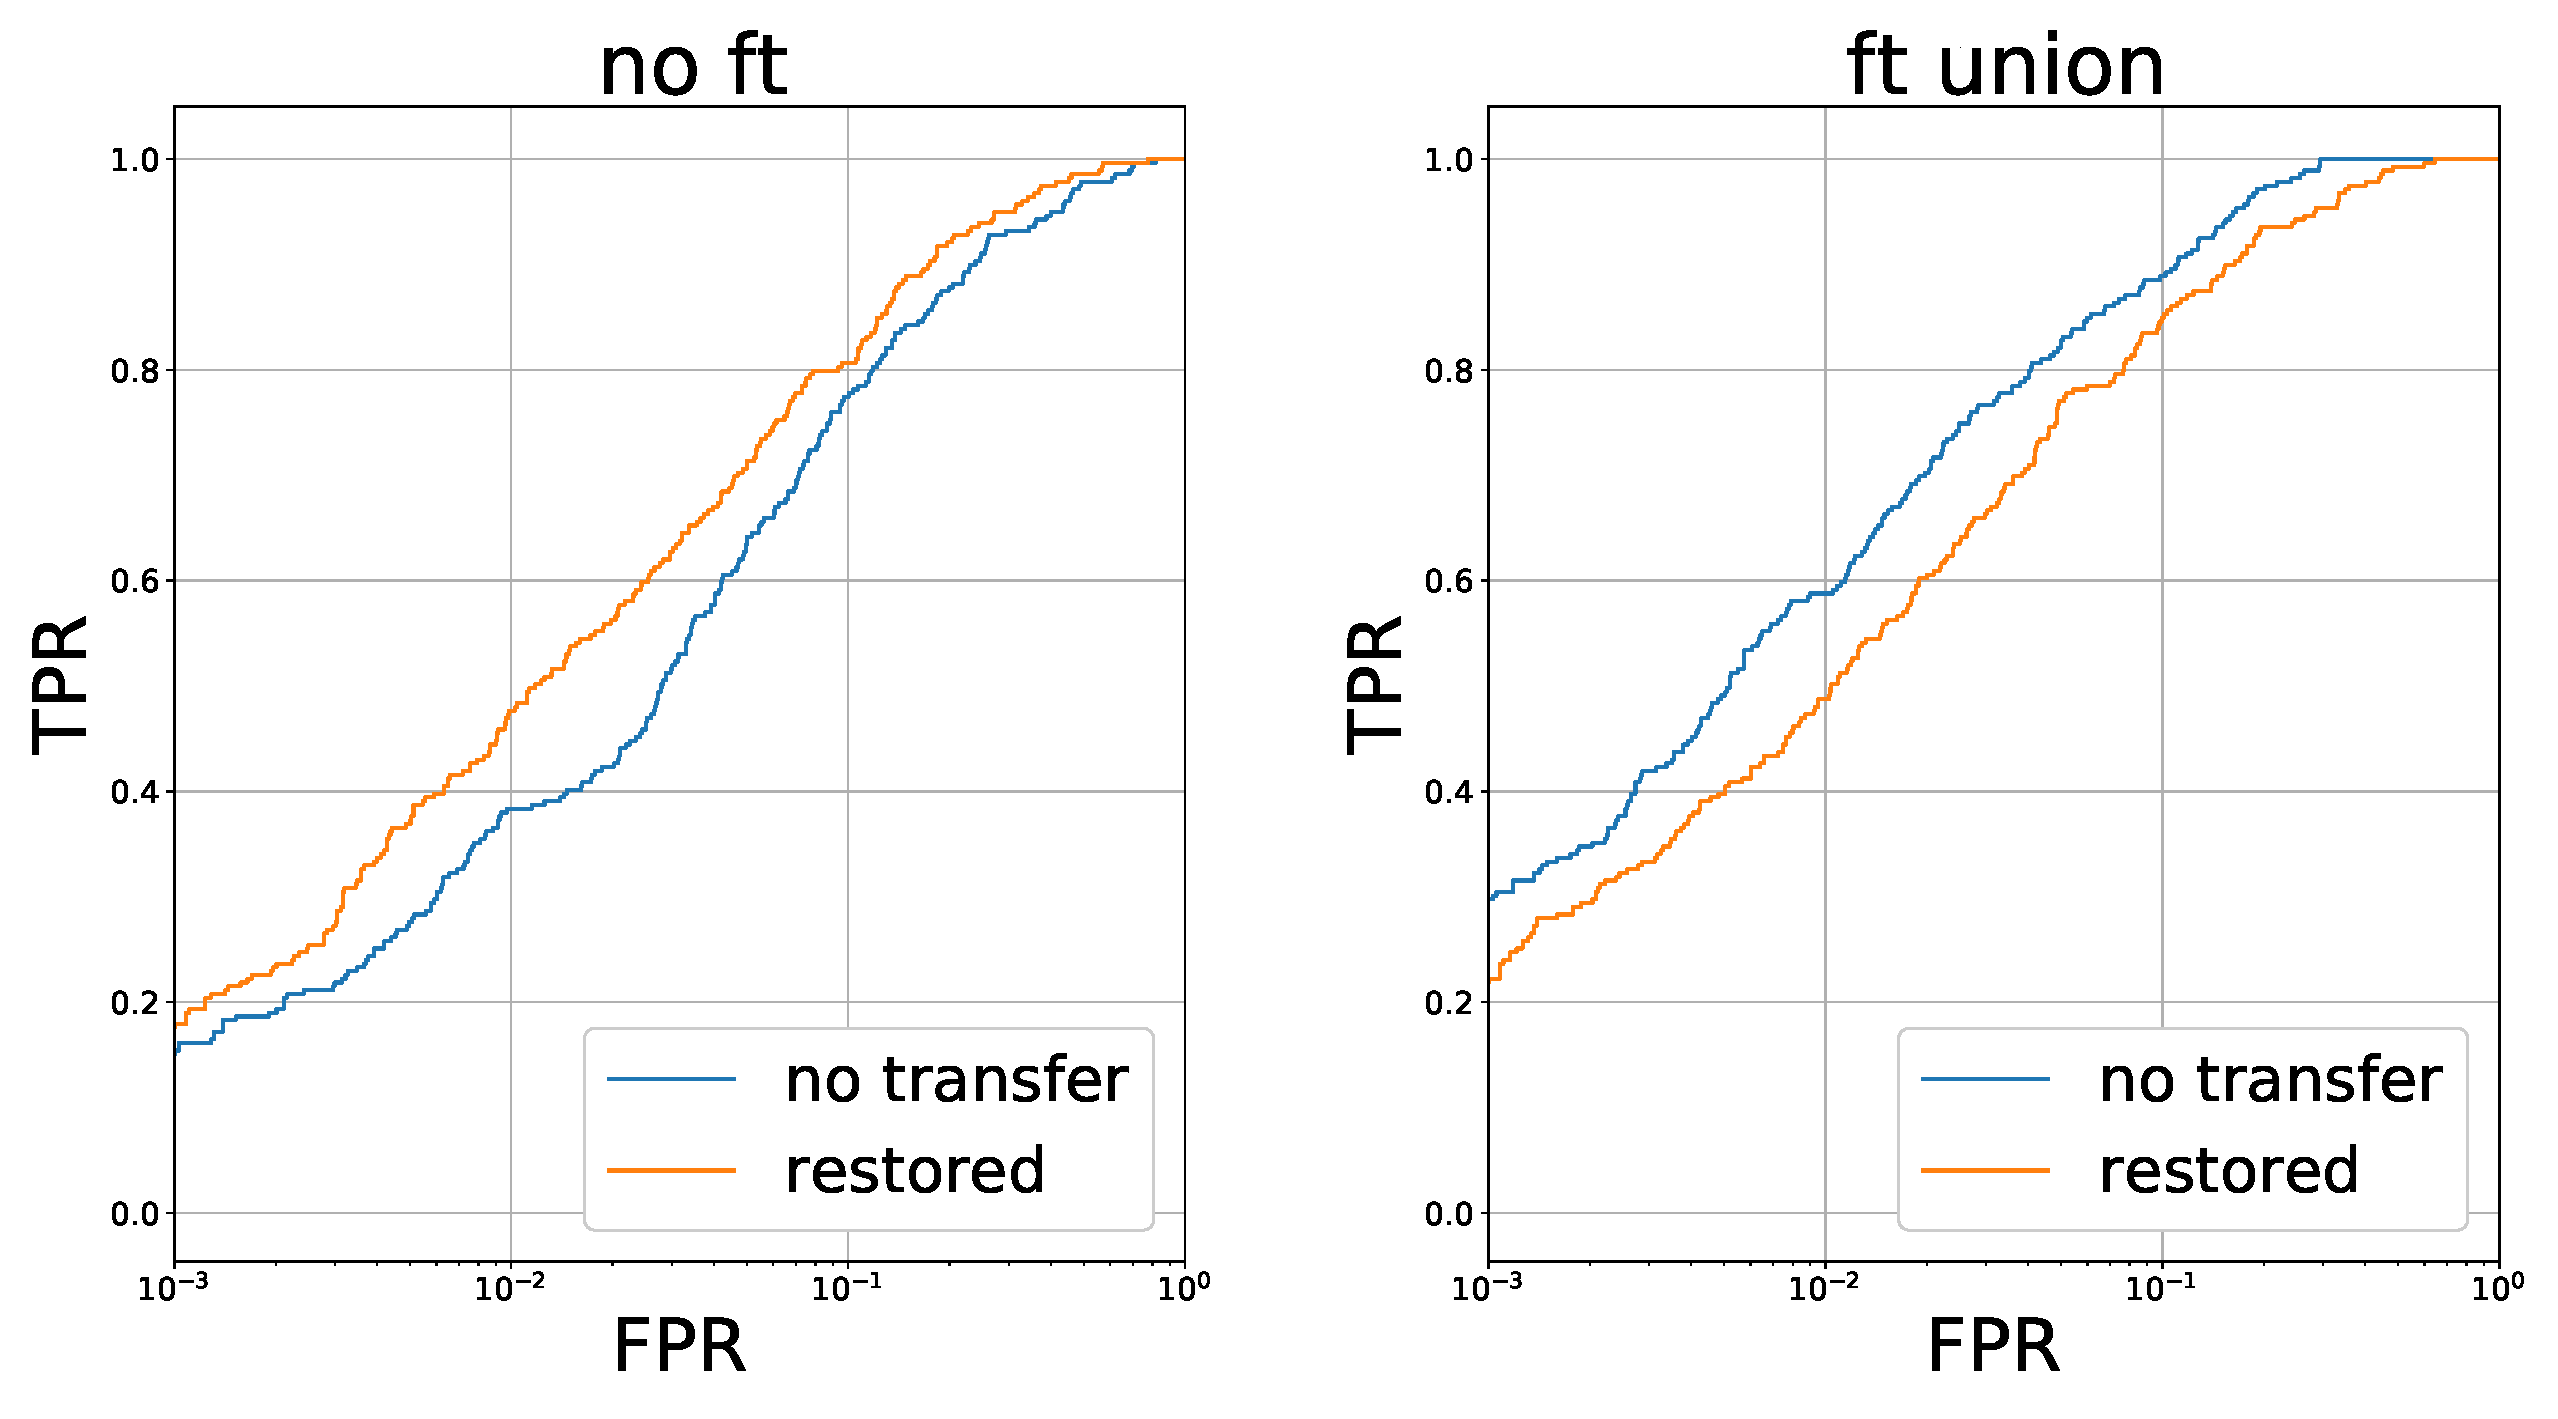
\includegraphics[width=\linewidth]{Chapters/facev1/Fig4.eps}
    \caption{The ROC curves for our face recognition models for different types of test data. Left -- \textit{no ft} model, test data transformation (the curve is denoted by 'restored') improves recognition. Middle -- \textit{ft initial}, the results for test data transformation are not clearly better than the results for initial images. Right -- \textit{ft union} model, the best results are for initial test data, without transformation. See \ref{sect:restoration_comparison} for the details. }\label{fig:roc_oxford_gan_vs_initial}
  \end{figure}

\newpage
\bigskip\indent\textbf{Does the translation to the Internet domain help recognition?} 
\label{sect:restoration_comparison}

We start by assessing the improvement that the restoration process brings to the recognition. For this we evaluate the performance of the three different recognition networks discussed above, when they are applied either to untransformed surveillance-domain images or to surveillance-domain images transformed to the Internet image domain (using the learned mapping $F^{A \rightarrow B}$). See  \fig{lr_hr_gan_res_ytube_initial_degraded} for the example results of the Internet domain  transfer.

The ROC-curves in  \fig{roc_oxford_gan_vs_initial} shows that while the restoration process helps for the \textit{no ft} network, it actually \textit{hurts} for the better-performing \textit{ft union} network. While trying to improve the results of the reverse transfer, we have also tried to transfer only the LR subset of the training images, while keeping the HR subset intact, but this lead to uniformly worse results.

We conclude that restoration does not necessarily help the recognition process in our setting. 

In the course of our experiments, we have also tried several different options for training CycleGAN. For example, we observed that the CycleGAN training scheme from \citep{ZhuPIE17} did not lead to visually good results for our data. Second, for the CycleGAN version mentioned in the paper, we have also tried an approach similar to that of \citep{sungatullina2018image}. In more details, we not only fed images to the higher-quality domain discriminator  $D^{I}$, but also intermediate features extracted from a pretrained face recognition network. As a result, we observed that ‘restoration’ transfer gave very visually plausible results, but recognition quality after such transform dropped considerably and was uniformly worse than all the results in \fig{roc_oxford_gan_vs_initial}. This might be due to non identity-preserving way of facial features change.


% \begin{figure}
%  \centering
%     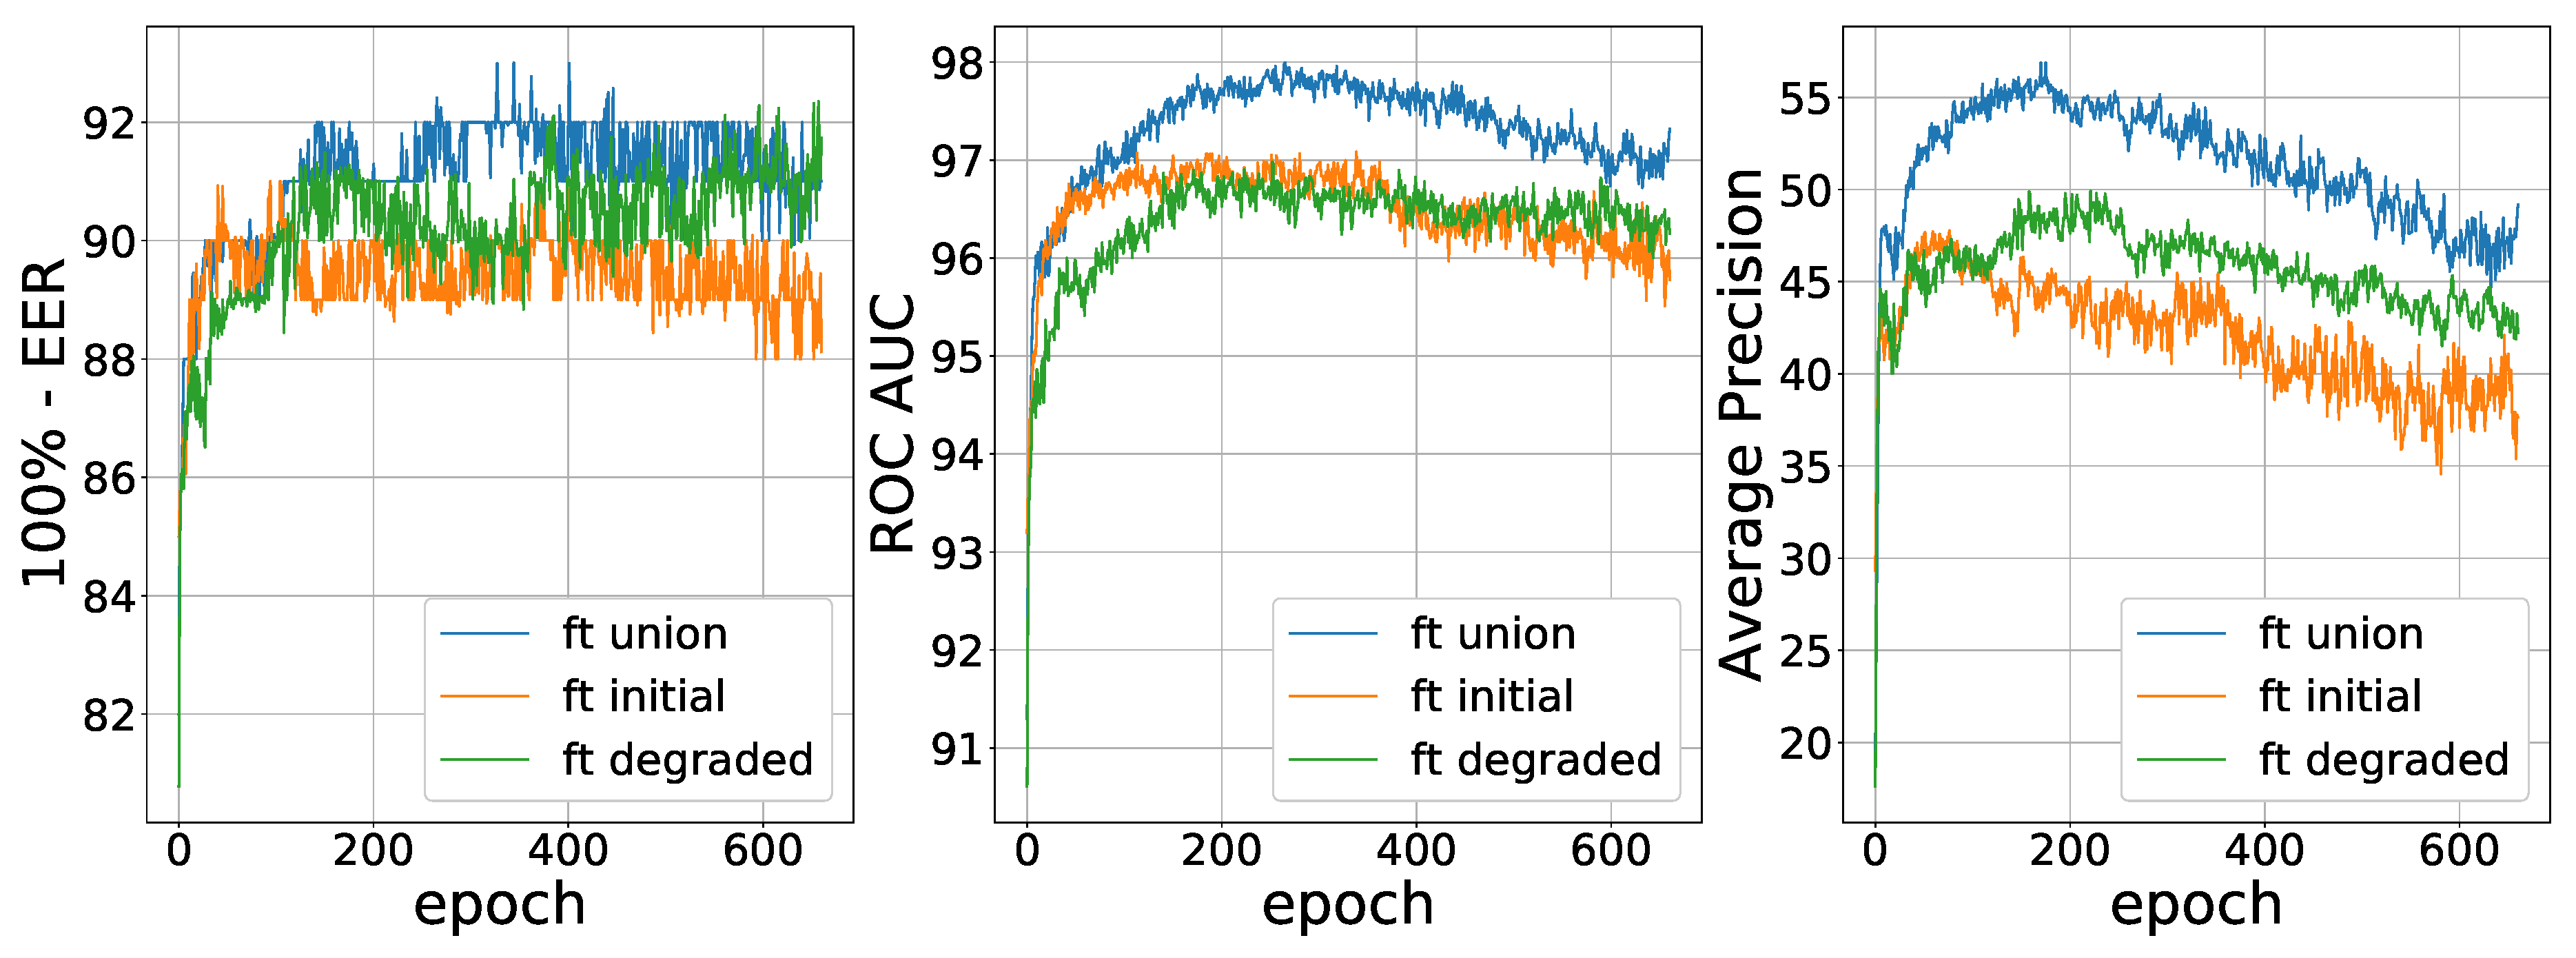
\includegraphics[width=\linewidth]{Fig4.eps}
%     \caption{The change of the recognition metrics for our surveillance validation set. \textit{ft degraded} and \textit{ft union} models that use our image-level domain adaptation overfit less than \textit{ft initial} that use only the initial Internet-domain data. The improvement is consistent across the two cases when VGG face and YTF datasets were used as Internet image data. See section \ref{sect:ft} for the models description.}\label{fig:validation_ytube}
%   \end{figure}
  
  \begin{figure}

  \centering
    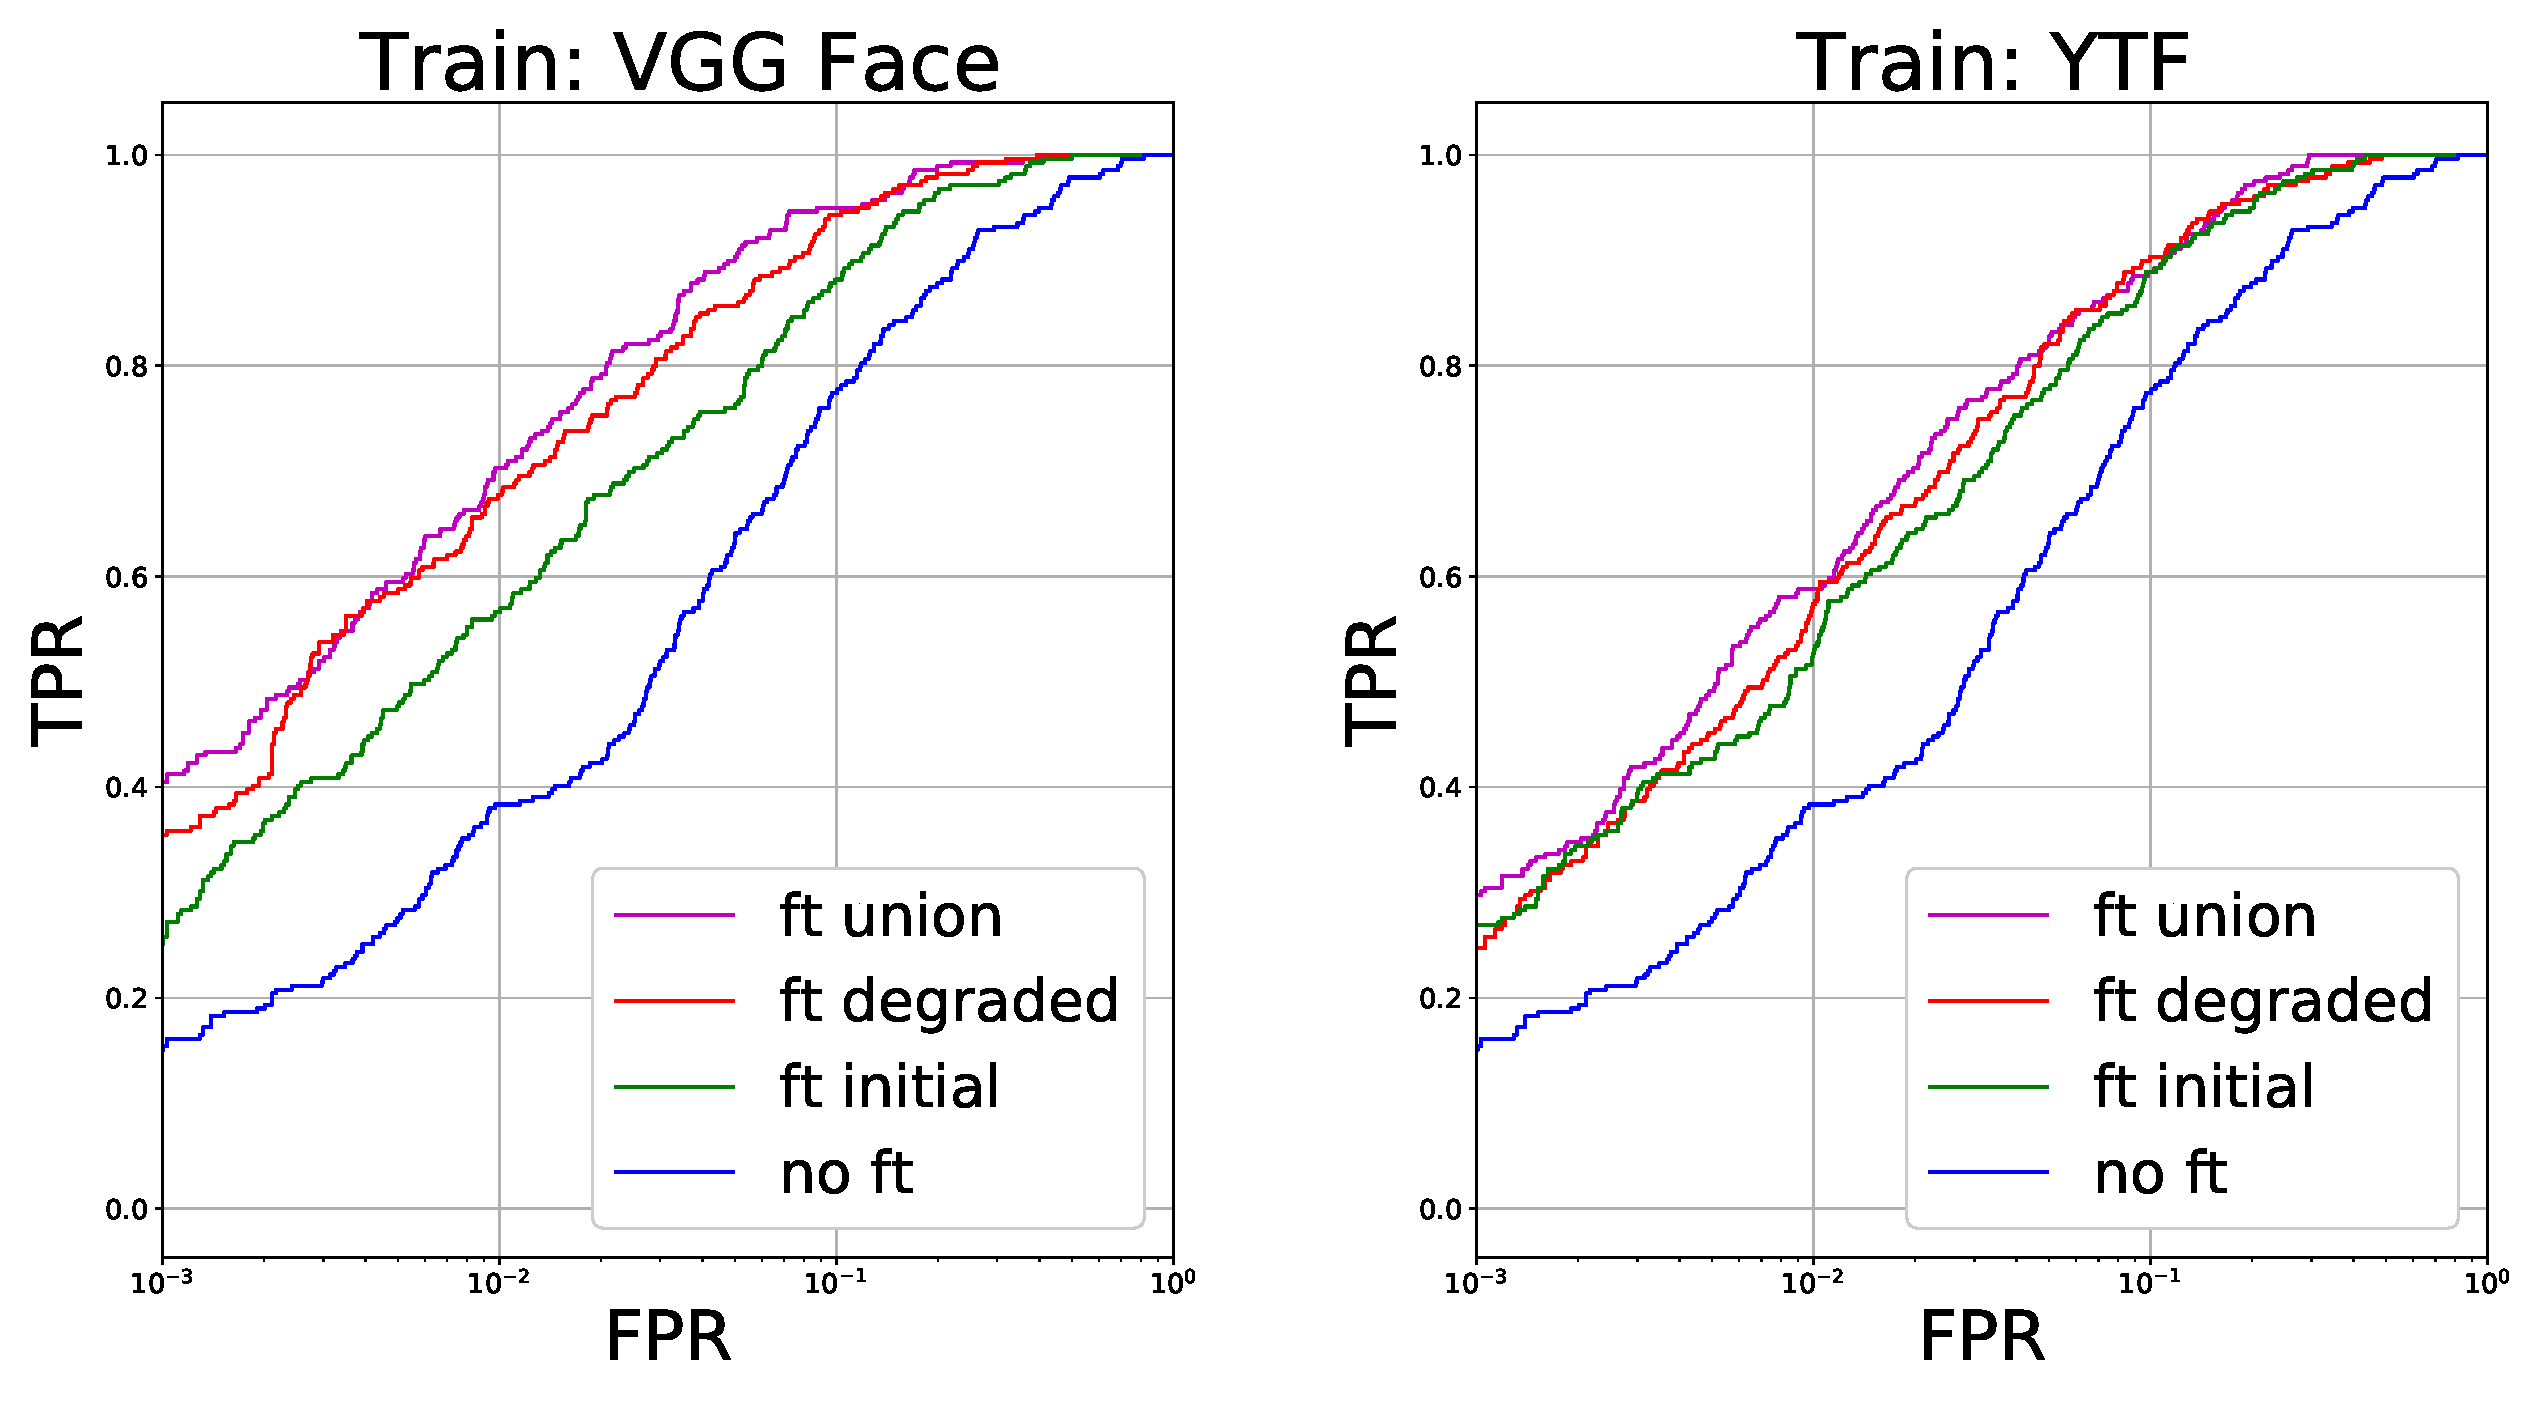
\includegraphics[width=\linewidth]{Chapters/facev1/Fig5.eps}
    \caption{The ROC curves for the fine-tuning strategies described in \sect{ft}. Our surveillance data is used for test. \textit{ft degraded} and \textit{ft union} models that use our image-level domain adaptation are better than other models. }\label{fig:roc_oxford_ytube}
  \end{figure}
  
 
\begin{table}
\centering
\flushbottom

\centering
\caption{Quality metrics for different face recognition models compared in this work (\ref{sect:ft}). Surveillance data are used for evaluation. The best model is \textit{ft union}, it is trained on both initial and degraded data.}
\label{tab:comparison}
\resizebox{0.7\columnwidth}{!}{
\begin{tabular}{c|ccc|ccc}
\hline
%\multicolumn{1}{|l|}{}   & \multicolumn{6}{c|}{Train datasets}                      \\ \hline
\multicolumn{1}{l|}{}   & \multicolumn{3}{c|}{train: VGG Face} & \multicolumn{3}{c}{train: YTF} \\ \hline
Fine-tuning type & 100\%$-$eer & roc auc & AP & 100\%$-$eer   & roc auc   & AP  \\ \hline
no ft                   &  83.89 & 91.86 & 22.04  &  83.89 & 91.86 & 22.04  \\ %\hline
ft initial               &  89.12 & 96.25 & 42.02  &  89.24 & 96.19 & 40.81 \\ %\hline
ft degraded             &  91.55 & 97.70 & 52.55 &  \bf{90.04} & 96.54 & 42.07   \\ %\hline
ft union                & \bf{92.94} &  \bf{98.08} & \bf{57.30}  &  89.37 & \bf{96.96} & \bf{45.45}      \\ \hline
\end{tabular}
}
\end{table}

  
  \begin{table}
\centering
\caption{Quality metrics of our approach compared to that of \citep{ganin2016domain} and \citep{SohnLZY0C17} and some combinations of these methods with ours. Surveillance data are used for evaluation. 'fm loss' and 'fr loss' stand for Feature Matching loss and Feature Reconstruction loss as defined in \citep{SohnLZY0C17}. 'adv loss' column shows if the method of \citep{ganin2016domain} for feature-level domain adaptation is used. 'aug type' column shows which augmentation method is used for each of the models: 'CycleGAN' means our CycleGAN based augmentation, 'predefined' means the procedure used in \citep{SohnLZY0C17}. The \textit{ft union} model is denoted A in this table. Model B combines feature-level ('adv loss') and image-level domain adaptation ('aug type' is set to 'CycleGAN'), it outperforms model A slightly. Overall, augmentation choice is very important: models D and I are trained using scheme from \citep{SohnLZY0C17} with different augmentation methods, and model D performs better than model I and on par with B.}
\label{tab:comparison_other}
\resizebox{0.7\columnwidth}{!}{
\begin{tabular}{cccccccc}
\hline
&fm loss & fr loss & adv loss & aug type & 100\% - eer    & roc auc        & AP             \\ \hline
\multicolumn{8}{c}{ours}                                                             \\ \hline
A &-  & -  & -   & CycleGAN          & 89.37          & \textbf{96.96} & 45.45          \\
B &-  & -  & \checkmark   & CycleGAN          & \textbf{89.75} & 96.72          & \textbf{46.22} \\
C &-  & -  & \checkmark   & -             & 88.30          & 95.63          & 39.01          \\
\hline
\multicolumn{8}{c}{our implementation of \citep{SohnLZY0C17}}                 \\ \hline
D &\checkmark  & \checkmark  & \checkmark   & CycleGAN        & \textbf{90.34} & \textbf{96.83} & \textbf{43.08} \\
E &-  & -  & \checkmark   & CycleGAN        & 89.26          & 96.52          & 42.75      \\
F &-  & \checkmark  & \checkmark   & CycleGAN        & 89.86          & 96.51          & 40.10         \\
G &\checkmark  & -  & \checkmark   & CycleGAN        & 88.05          & 96.06          & 40.89          \\
H &\checkmark  & \checkmark  & -   & CycleGAN        & 89.79          & 96.76          & 42.56          \\ \hline
I &\checkmark  & \checkmark  & \checkmark   & predefined            & \textbf{89.22}          & \textbf{96.16}          & \textbf{40.66} \\
J &-  & -  & \checkmark   & predefined            & 88.69          & 95.92          & 38.92 \\ \hline

\end{tabular}
}
\end{table}
 
\bigskip\indent\textbf{Does domain adaptation help recognition?}\\
\label{sect:results}

We now consider the second scenario based on domain adaptation and thus compare the performance of different recognition networks described above on surveillance data. Our findings for image level domain adaptation are summarized in Table~\ref{tab:comparison}, which shows metric values for the compared training settings. Finally, \fig{roc_oxford_ytube} shows the final ROC curves.

The following can be observed. First, fine-tuning the VGG Face model on either VGG Face dataset or the YTF dataset using the BinDev loss (\textit{ft initial}) lead to a considerable improvement over the original state of the network.
Furthermore, we found that fine-tuning in the \textit{ft degraded} setting is clearly beneficial compared to \textit{ft initial} setting in the case of the VGG Face training dataset, and a little bit better for the YTF training data, overall making a case for image-level domain adaptation. The results of the \textit{ft union} setting are uniformly better than \textit{ft initial} and \textit{ft degraded} suggesting that the automatically degraded data are a useful augmentation, but that the original data should not be discarded. 

Finally, \fig{tsne} shows that the feature distribution of our surveillance data is more intermixed with those of the degraded version of the YTF dataset than its initial version. This aligns with the performance improvement we achieved with image-level domain adaptation.
%Finally, \fig{tsne} gives an additional evidence of the success of domain adaptation. It shows that the feature distribution of our surveillance data is more intermixed with those of the degraded version of the YTF dataset than its initial version. This demonstrates the relevance of the suggested augmentation (via image-level domain adaptation).



% \subsection{Comparison to the reverse domain transfer}
% \label{sect:restoration_comparison}

% We have also investigated the restoration-based approach (\sect{strategies}), using the reverse mapping $F^{B \rightarrow A}$ that also comes out as the result of training the model \ref{sect:domain_transfer}. 
% Here we test our previously trained face recognition models (described in  \sect{ft}) on different variants of test data. See  \fig{lr_hr_gan_res_ytube_initial_degraded} for the example results of the Internet domain  transfer.

% We have evaluated the effect of such reverse transfer to the higher-quality domain at test term for the \textit{no ft}, \textit{ft initial}, and \textit{ft union} networks described in the previous section. The ROC-curves in  \fig{roc_oxford_gan_vs_initial} shows that while the reverse transfer helps for the \textit{no ft} network, it actually hurts for the better working \textit{ft initial} and \textit{ft union} networks. While trying to improve the results of the reverse transfer, we have also tried to transfer only the LR subset of the training images, while keeping the HR subset intact, but this lead to uniformly worse results.

%in the case of the pre-trained VGG face network (\textit{no-ft}), transferring low-quality test images into the Internet data domain improves recognition. Nevertheless, if we use one of the fine-tuned models for recognition, the results for the initial test images are not worse than those for transferred images. Moreover, ROC curve for initial test images is the highest for our best \textit{ft union} model as shown in \ref{fig:roc_oxford_gan_vs_initial}-right.

\bigskip\indent\textbf{Comparison to other domain adaptation methods}\\
\label{sect:grl}
We have additionally compared our image-level domain adaptation (all the experiments and discussions above) to the feature-level domain-adversarial adaptation approach~\citep{ganin2016domain} as well as to the approach described in \citep{SohnLZY0C17}.


\citep{ganin2016domain} proposes a feature-level adaptation technique based on reversing the sign of gradients of the domain discriminator with respect to the intermediate representations in order to make those representations more domain-invariant.  
We thus built a DANN (Deep Adversarial Neural Network) based on the VGG-face network. The  domain classifier consists of three fully-connected layers: $512$ units in the first two layers (Leaky ReLU \citep{HeZRS15} non-linearities were used) and one classification layer with $1$ unit. Dropout with $0.5$ probability was inserted before the classification layer. The Gradient Reversal layer is attached after the \textit{fc6} layer of VGG-face. We found that schedule for the adaptation parameter  $\lambda$ is very important for this task. Instead of the schedule suggested in \citep{ganin2016domain} (which did not lead to good results in our comparison), we set $\lambda$ to $1e-3$ and increased it to $1e-2$ and $1e-1$ after the first and the fifth epochs correspondingly. In these experiments,  we fine-tune one of our pre-trained models (either \textit{ft initial} or \textit{ft union}) with additional feature-level domain adaptation objective. 

   \begin{figure}
  \centering
    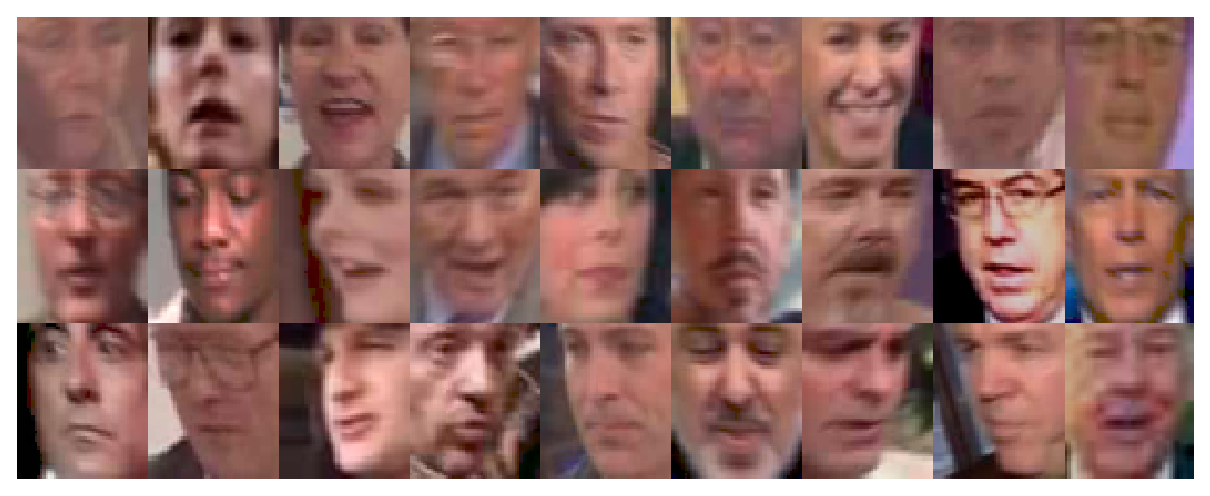
\includegraphics[width=\linewidth]{Chapters/facev1/Fig7.eps}
    \caption{Examples of degraded images produced using a predefined procedure from \citep{SohnLZY0C17}. See \tab{comparison_other} for comparison with our augmentation. }\label{fig:predefined}
  \end{figure}
  
The results for training on the YTF dataset with  method \citep{ganin2016domain} are shown in \tab{comparison_other}: 
model A corresponds to our \textit{ft union} model, model B combines the image-level domain-adaptation (the same as for \textit{ft union}) and feature-level domain adaptation, model C uses feature-level domain adaptation only. Feature-level domain adaptation improves the performance slightly if combined with the image-level domain adaptation (model B compared to model A), whereas applied alone, it leads to overfitting (model C).

We have also compared our approach to the method described in \citep{SohnLZY0C17}. It aims at performing feature-level adaptation and restoration using artificially-degraded data as a bridge between the two domains. The goal is to train such a model that would be tolerant to image degradation and at the same time, retain the representations of the source domain data. 
The authors also incorporate a feature-level adversarial loss, and we use that of \citep{ganin2016domain} for our implementation of \citep{SohnLZY0C17} for better comparability. Instead of the Image Classification loss used in \citep{SohnLZY0C17}, we use the BinDev loss as for the other experiments in this work.
Two other losses that were used in \citep{SohnLZY0C17}, apart for Image Classification loss and Domain-Adversarial loss, are Feature Matching and Feature Restoration losses. To implement the scheme from \citep{SohnLZY0C17}, we added these two losses to the final objective function. Additionally, it should be noted that in \citep{SohnLZY0C17}, the network is initialised by the weights of the model trained on the source domain (\textit{ft initial} in our case). We also used the predefined degradation procedure described in \citep{SohnLZY0C17} to generate augmentation data.
%todo insert a picture with examples

The results of our implementation of the scheme from \citep{SohnLZY0C17} are shown in \tab{comparison_other} in rows D-J. All the models D-J are fine-tuned with additional losses from \citep{SohnLZY0C17} (with changes discussed above) starting at the state of \textit{ft inital}. Models D and I differ in the utilized augmentation method. Model I uses pre-defined augmentation procedure ('predefined', see \fig{predefined} for examples) from \citep{SohnLZY0C17}, whereas our CycleGAN-based augmentation is used for D.  We can see that our augmentation results in better performance in comparison to that of \citep{SohnLZY0C17} for our data. We also compared the two augmentation methods for our training scheme \textit{ft-union} and observed very similar results (not shown here).
 To ensure the sanity of our implementation of \citep{SohnLZY0C17}, we also show the role of different subsets of losses in the rows D-H of \tab{comparison_other}. Indeed, we can see that model D, that is trained with the full set of losses, outperforms other models E-H. 

Finally, we can see from \tab{comparison_other}, that our approach (models A and B) outperforms the scheme from \citep{SohnLZY0C17} (model I), and as it can be seen from the comparison, the difference mostly comes from the augmentation method: model D is trained using our CycleGAN-based augmentation and the resulting performance is close to that of our model B.
 


% \subsection{Comparison to feature-level domain adaptation}
% \label{sect:grl}
% We have additionally compared our image-level domain adaptation (all the experiments and discussions above) to the feature-level domain-adversarial adaptation approach~\citep{ganin2016domain}. Tuning this approach required some effort (several modifications from the settings of~\citep{ganin2016domain} were needed to make such adaptation work). We thus built a DANN (Deep Adversarial Neural Network) based on the VGG-face network. The  domain classifier consists of three fully-connected layers: $512$ units in the first two layers (Leaky ReLU \citep{HeZRS15} non-linearities were used) and one classification layer with $1$ unit. Dropout with $0.5$ probability was inserted before the classification layer. The Gradient Reversal layer is attached after the \textit{fc6} layer of VGG-face. We found that schedule for the adaptation parameter  $\lambda$ is very important for this task. Instead of the schedule suggested in \citep{ganin2016domain} (which did not lead to good results in our comparison), we set $\lambda$ to $1e-3$ for the first $20$ epochs and then increased it to $1e-2$. 

% Using the scheme described above when training on the VGG Face dataset, we have achieved the following results: $100$\% - EER was $88.64$, ROC AUC was $96.69$ and the average precision was $52.11$. This is better than the results of our \textit{ft initial} setting, but worse than those of \textit{ft degraded} and \textit{ft union} settings (for the last, the results are $91.31$, $97.80$ and $54.89$ correspondingly). Other setting for feature-level domain adaptation that we have tried lead to worse results.






  
  
  
  


 

  \begin{figure}
  \centering
    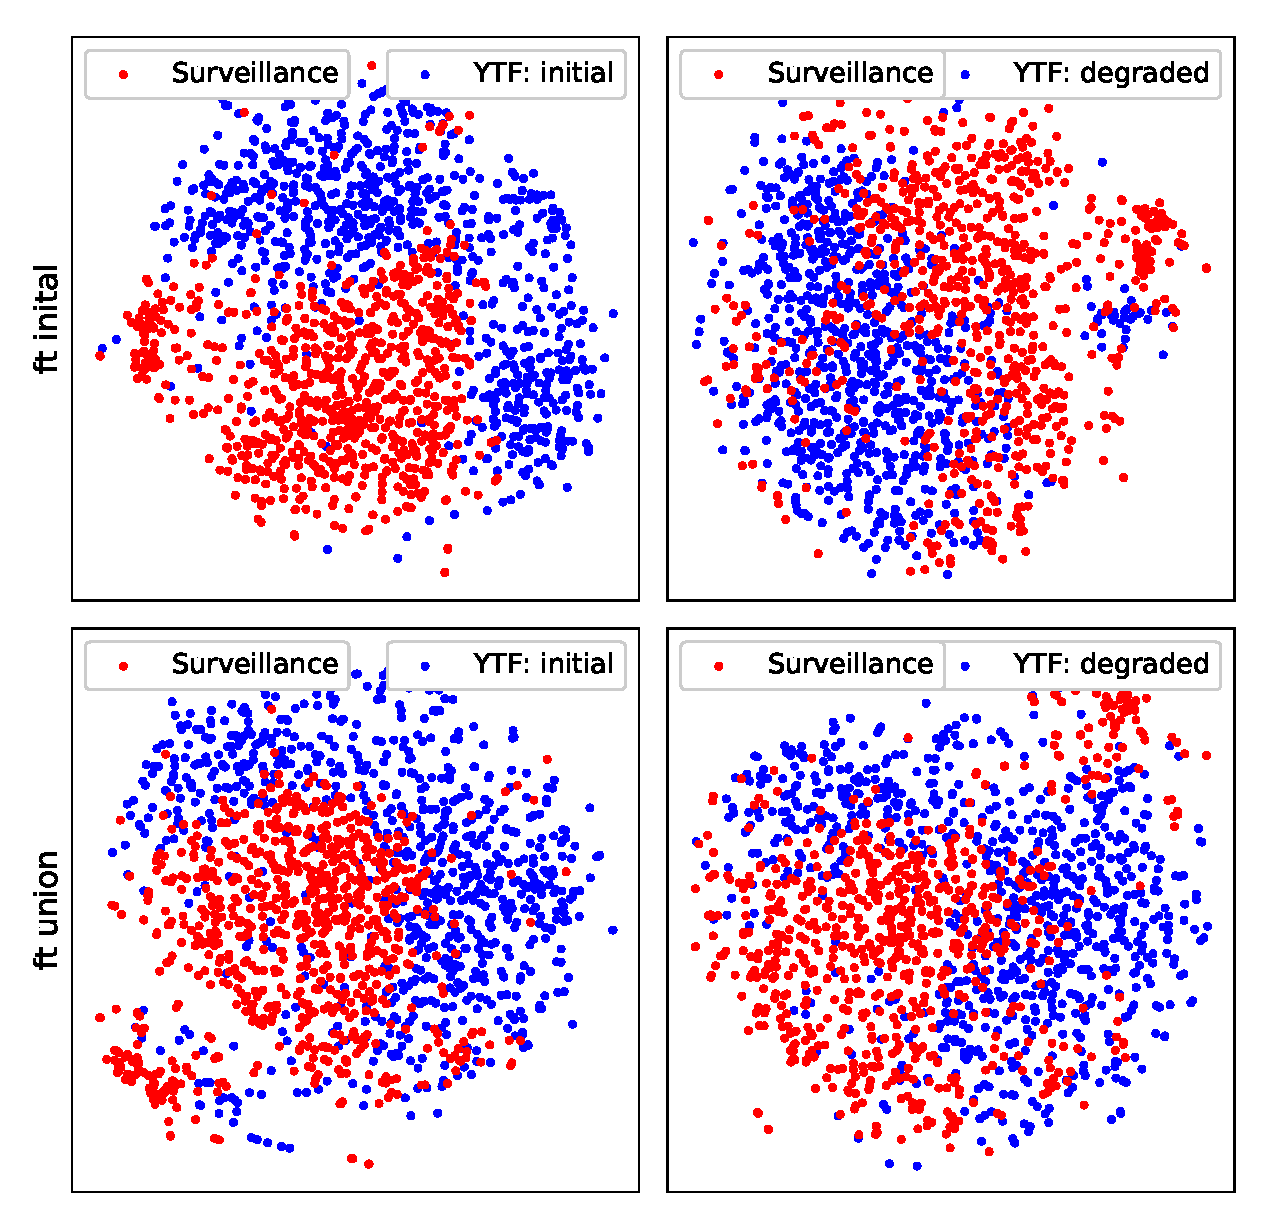
\includegraphics[width=\linewidth]{Chapters/face/Fig6.eps}
    \caption{t-SNE \citep{maaten2008visualizing} visualizations for deep features extracted with: first row -- \textit{ft initial}, second row -- \textit{ft union} neural nets (See \ref{sect:ft} for the descriptions of the models). For both nets, surveillance data distribution is more intermixed with the degraded version of the YTF dataset than with its initial version.}\label{fig:tsne}
  \end{figure}


\section{Discussion and Conclusions}
\label{sect:conclusion}

% Discuss your conclusions in order of most to least important.

 In this chapter, we have compared the image-based domain adaptation techniques for face recognition in the presence of strong image degradation. We consider the recently proposed CycleGAN approach for learning mappings between the two domains of surveillance data and Internet face images. We demonstrate that the strategy of transferring the labeled Internet data to the surveillance domain and subsequent retraining the face recognition network helps to improve the recognition quality on real surveillance test data. We have investigated the variants of this approach, and have demonstrated that training on both transferred and original Internet data leads to the optimal performance. Finally, we show that in the case of our domain pair, the image-level adaptation approach outperforms feature-level domain adaptation. 

%Compare your results with those from other studies: Are they consistent? If not, discuss possible reasons for the difference.
 We found our results consistent with \citep{SohnLZY0C17}, where face recognition for the low-quality is also considered. In \citep{SohnLZY0C17},  verification accuracy was improved using carefully chosen data augmentation. However, we also show that for our data, the approach analogical to \citep{SohnLZY0C17} benefits considerably from using our automatic augmentation. 
 %It is an interesting fact, that the improvement remained noticeable even when the data augmentation and the feature-level domain adaptation were applied simultaneously. Here, in contrast, we suggest performing the data augmentation in a more automatic way. Although we do not experiment with the combination of feature-level and image-level approaches to domain adaptation, we compare them independently. The combination of these adaptation techniques may further improve the results.


% Mention any inconclusive results and explain them as best you can. You may suggest additional experiments needed to clarify your results.
In our experiments, best results were achieved with training on both domains. An explanation can be given that the domain transfer model is imperfect and may push different images of the same identity too far as we do not use any kind of verification loss for training (ideally, this would require another pre-trained network for the low-quality domain, which essentially is the goal of this work). Therefore, keeping the initial data in the training set may result in less overfitting. %This can be explained by the fact that our target domain is not uniform in terms of data quality. We use two parts of the same track to generate matching pairs for each identity: e.g. these parts of each track differ in resolution (see \ref{fig:lr_hr_gan_res_ytube_initial_degraded}, columns $1$ and $3$). Therefore, using training data of diverse quality may lead to better results.  -- not true, checked.

% Briefly describe the limitations of your study to show reviewers and readers that you have considered your experiment’s weaknesses. Many researchers are hesitant to do this as they feel it highlights the weaknesses in their research to the editor and reviewer. However doing this actually makes a positive impression of your paper as it makes it clear that you have an in depth understanding of your topic and can think objectively of your research.

As an important negative result, we show that using CycleGAN-based restoration of lower-quality domain images by transferring them to the higher-quality domain does not bring consistent improvement to the recognition performance, which is also consistent with the results of \citep{SohnLZY0C17}. We speculate that such transfer may distort some details of the images in a non-identity preserving way.

Our study considers a practically important domain of image data. 
We note, however, that our findings might not transfer to other pairs of domains in image adaptation as optimal strategies may vary for different domains of data. Here were are experimenting with the two domains, one of which is associated with the information loss, including identity information crucial for our main task (face verification). In our case, the strategy of translation from the target domain to the source domain (\‘restoration\’) did not quite work, or it was harder to make it work than the opposite approach. However, this strategy might be more applicable to some other domains, e.g. high-quality city photos and synthetic city images.



% Discuss what your results may mean for researchers in the same field as you, researchers in other fields, and the general public. How could your findings be applied?
 
% State how your results extend the findings of previous studies.
% If your findings are preliminary, suggest future studies that need to be carried out.
% At the end of your Discussion and Conclusions sections, state your main conclusions once again.


\textbf{Acknowledgement:}  This research is supported by VisionLabs and the Ministry of Education and Science of the Russian Federation (grant 14.756.31.0001). 

% \appendix
% \section{Feature-level domain adaptation settings}
% \label{sect:app_grl}
% Here we describe the settings for the feature-level domain adaptation (used in the comparison of Section~ \ref{sect:grl}). We built a DANN (Deep Adversarial Neural Network) based on the VGG-face network. The  domain classifier consists of three fully-connected layers: $512$ units in the first two layers (Leaky ReLU \cite{HeZRS15} non-linearities were used) and one classification layer with $1$ unit. Dropout with $0.5$ probability was inserted before the classification layer. The Gradient Reversal layer is attached after the \textit{fc6} layer of VGG-face. We found that schedule for the adaptation parameter \lamdba is very important for this task. Instead of the schedule suggested in \cite{GaninUAGLLML16} (which did not lead to good results in our comparison), we set \labmda to $1e-3$ for the first $20$ epochs and then increased it to $1e-2$. 




%\begin{acknowledgements}
%If you'd like to thank anyone, place your comments here
%and remove the percent signs.
%\end{acknowledgements}

% BibTeX users please use one of
%\bibliographystyle{spbasic}      % basic style, author-year citations
%\bibliographystyle{spmpsci}      % mathematics and physical sciences
%\bibliographystyle{spphys}       % APS-like style for physics

%\bibliography{main}


% end of file template.tex


% \newpage 
% 
\section{Conclusion}
\label{sect:conclusion}

% Discuss your conclusions in order of most to least important.

In this chapter, we have compared the image-based domain adaptation techniques for face recognition in the presence of strong image degradation. We consider the recently proposed CycleGAN approach for learning mappings between the two domains of surveillance data and Internet face images. We demonstrate that the strategy of transferring the labeled Internet data to the surveillance domain and subsequent retraining the face recognition network helps to improve the recognition quality on real surveillance test data. We have investigated the variants of this approach, and have demonstrated that training on both transferred and original Internet data leads to the optimal performance. Finally, we show that in the case of our domain pair, the image-level adaptation approach outperforms feature-level domain adaptation. 

%Compare your results with those from other studies: Are they consistent? If not, discuss possible reasons for the difference.
We found our results consistent with \cite{SohnLZY0C17}, where face recognition for the low-quality is also considered. In \cite{SohnLZY0C17},  verification accuracy was improved using carefully chosen data augmentation. It is an interesting fact, that the improvement remained noticeable even when the data augmentation and the feature-level domain adaptation were applied simultaneously. Here, in contrast, we suggest performing the data augmentation in a more automatic way. Although we do not experiment with the combination of feature-level and image-level approaches to domain adaptation, we compare them independently. The combination of these adaptation techniques may further improve the results.


% Mention any inconclusive results and explain them as best you can. You may suggest additional experiments needed to clarify your results.
In our experiments, best results were achieved with training on both domains. An explanation can be given that the domain transfer model is imperfect and may push different images of the same identity too far as we do not use any kind of verification loss for training (ideally, this would require another pre-trained network for the low-quality domain, which essentially is the goal of this work). Therefore, keeping the initial data in the training set may result in less overfitting. %This can be explained by the fact that our target domain is not uniform in terms of data quality. We use two parts of the same track to generate matching pairs for each identity: e.g. these parts of each track differ in resolution (see \ref{fig:lr_hr_gan_res_ytube_initial_degraded}, columns $1$ and $3$). Therefore, using training data of diverse quality may lead to better results.  -- not true, checked.

% Briefly describe the limitations of your study to show reviewers and readers that you have considered your experiment’s weaknesses. Many researchers are hesitant to do this as they feel it highlights the weaknesses in their research to the editor and reviewer. However doing this actually makes a positive impression of your paper as it makes it clear that you have an in depth understanding of your topic and can think objectively of your research.

As an important negative result, we show that using CycleGAN-based restoration of lower-quality domain images by transferring them to the higher-quality domain does not bring consistent improvement to the recognition performance. We speculate that such transfer may distort some details of the images in a non-identity preserving way.

Our study considers a practically important domain of image data. 
We note, however, that our findings might not transfer to other pairs of domains in image adaptation.


% Discuss what your results may mean for researchers in the same field as you, researchers in other fields, and the general public. How could your findings be applied?
 
% State how your results extend the findings of previous studies.
% If your findings are preliminary, suggest future studies that need to be carried out.
% At the end of your Discussion and Conclusions sections, state your main conclusions once again.



%% ----------------------------------------------------------------
% Now begin the Appendices, including them as separate files

\addtocontents{toc}{\vspace{2em}} % Add a gap in the Contents, for aesthetics

\appendix 

%\mbox{}
 



% Cue to tell LaTeX that the following 'chapters' are Appendices

%\chapter{An Appendix}

Lorem ipsum dolor sit amet, consectetur adipiscing elit. Vivamus at pulvinar nisi. Phasellus hendrerit, diam placerat interdum iaculis, mauris justo cursus risus, in viverra purus eros at ligula. Ut metus justo, consequat a tristique posuere, laoreet nec nibh. Etiam et scelerisque mauris. Phasellus vel massa magna. Ut non neque id tortor pharetra bibendum vitae sit amet nisi. Duis nec quam quam, sed euismod justo. Pellentesque eu tellus vitae ante tempus malesuada. Nunc accumsan, quam in congue consequat, lectus lectus dapibus erat, id aliquet urna neque at massa. Nulla facilisi. Morbi ullamcorper eleifend posuere. Donec libero leo, faucibus nec bibendum at, mattis et urna. Proin consectetur, nunc ut imperdiet lobortis, magna neque tincidunt lectus, id iaculis nisi justo id nibh. Pellentesque vel sem in erat vulputate faucibus molestie ut lorem.

Quisque tristique urna in lorem laoreet at laoreet quam congue. Donec dolor turpis, blandit non imperdiet aliquet, blandit et felis. In lorem nisi, pretium sit amet vestibulum sed, tempus et sem. Proin non ante turpis. Nulla imperdiet fringilla convallis. Vivamus vel bibendum nisl. Pellentesque justo lectus, molestie vel luctus sed, lobortis in libero. Nulla facilisi. Aliquam erat volutpat. Suspendisse vitae nunc nunc. Sed aliquet est suscipit sapien rhoncus non adipiscing nibh consequat. Aliquam metus urna, faucibus eu vulputate non, luctus eu justo.

Donec urna leo, vulputate vitae porta eu, vehicula blandit libero. Phasellus eget massa et leo condimentum mollis. Nullam molestie, justo at pellentesque vulputate, sapien velit ornare diam, nec gravida lacus augue non diam. Integer mattis lacus id libero ultrices sit amet mollis neque molestie. Integer ut leo eget mi volutpat congue. Vivamus sodales, turpis id venenatis placerat, tellus purus adipiscing magna, eu aliquam nibh dolor id nibh. Pellentesque habitant morbi tristique senectus et netus et malesuada fames ac turpis egestas. Sed cursus convallis quam nec vehicula. Sed vulputate neque eget odio fringilla ac sodales urna feugiat.

Phasellus nisi quam, volutpat non ullamcorper eget, congue fringilla leo. Cras et erat et nibh placerat commodo id ornare est. Nulla facilisi. Aenean pulvinar scelerisque eros eget interdum. Nunc pulvinar magna ut felis varius in hendrerit dolor accumsan. Nunc pellentesque magna quis magna bibendum non laoreet erat tincidunt. Nulla facilisi.

Duis eget massa sem, gravida interdum ipsum. Nulla nunc nisl, hendrerit sit amet commodo vel, varius id tellus. Lorem ipsum dolor sit amet, consectetur adipiscing elit. Nunc ac dolor est. Suspendisse ultrices tincidunt metus eget accumsan. Nullam facilisis, justo vitae convallis sollicitudin, eros augue malesuada metus, nec sagittis diam nibh ut sapien. Duis blandit lectus vitae lorem aliquam nec euismod nisi volutpat. Vestibulum ornare dictum tortor, at faucibus justo tempor non. Nulla facilisi. Cras non massa nunc, eget euismod purus. Nunc metus ipsum, euismod a consectetur vel, hendrerit nec nunc.	% Appendix Title

%\input{Appendices/AppendixB} % Appendix Title

%\input{Appendices/AppendixC} % Appendix Title

\addtocontents{toc}{\vspace{2em}}  % Add a gap in the Contents, for aesthetics
\backmatter

%% ----------------------------------------------------------------
\label{Bibliography}
\lhead{\emph{Bibliography}}  % Change the left side page header to "Bibliography"
\bibliographystyle{plainnat}  % Use the "unsrtnat" BibTeX style for formatting the Bibliography
\bibliography{Bibliography}  % The references (bibliography) information are stored in the file named "Bibliography.bib"


\begin{titlepage}
 \begin{center}
 \phantom{a}\vspace{13.2cm}
 

\includegraphics[width=6cm]{sk.png}
  
 
  \vspace{7cm}
  
  2020

  \vspace{2cm}

  
  
  
 \end{center}

\end{titlepage}
\end{document}  % The End
%% ---------------------------------------------------------------- 
